\section*{Supporting Information}

\subsection*{Molecular dating: calibrations and topological constraints}

% \noindent We followed three general guidelines in calibrating the
% divergence-time analyses with node age constraints. All were intended
% to be conservative with respect to constraining the maximum age of any
% given clade.

% \begin{enumerate}

% \item We used the earliest confirmed fossil record of a group to
%   constrain its minimum \textit{stem} age; most fossil species are
%   published based on fragmentary material that lack enough characters
%   to be placed within the crown group.

% \item We applied uniform priors to all calibrations.% , despite the
%   % effect of inferred node age confidence intervals being larger than
%   % for other commonly-used distributions, e.g.\ lognormal, exponential,
%   % etc. We believe current knowledge on fossils only allow us to make
%   % an assumption that one clade could originate at any time between the
%   % minimum and maximum bounds.

% \item We used 125 Myr, the age of the earliest eudicot fossil
%   \citep{Hughes1994}, to constrain the maximum age of angiosperm
%   clades in the absence of other evidence.
% \end{enumerate}

Below we list and explain the node age constraints used in calibrating
the divergence-time analyses in BEAST. For each analysis, the ingroup
is the taxon for which divergence times and ancestral geographic
ranges were reconstructed; the ``outgroup scope'' is the
least-inclusive taxon containing the ingroup and outgroup
taxa. Included in the list are fossil-calibrated ``backbone'' analyses
that we ran to derive secondary calibrations for some ingroups. A
spreadsheet containing taxon-by-gene tables of Genbank accession
numbers for all analyses is available as Dataset S1.

% \todo[inline]{\textit{Note to editor: BEAST XML files (containing the aligned
%   sequence data, Bayesian priors, and analysis directives) and the
%   results (maximum clade-credibility trees) can be provided as SI or
%   via Dryad.}}

Unless otherwise noted, the age ranges are the bounds of a uniform
prior distribution, and the nodes in question were topologically
constrained to be monophyletic. Wherever possible, we used fossils to
set the minimum (lower) bounds for these priors. For eudicot
angiosperm nodes, we set the upper (older) bound to 125 Ma, the age of
the earliest eudicot fossil \citep{Hughes1994}, if no other evidence
was available for a younger constraint.

\subsubsection*{Ingroup: \textit{Acer}; outgroup context: Sapindaceae}

% The analysis included 118 ingroup species and 2 outgroups,
% \textit{Dipteronia dyeriana} and \textit{D.~sinensis}.

\begin{enumerate}

\item \textbf{Stem age of \textit{Dipteronia}:} 60--125 Ma. The
  lower bound is based on the earliest fossil of
  \textit{Dipteronia}, winged fruits from the Paleocene of North
  America \citep{McClain2001}.

\item \textbf{Crown age of \textit{Acer}:} 47.8--125 Ma. \textit{Acer}
  has a rich fossil record, dating to at least the Paleocene
  \citep{Wolfe1987,Mai1995}. We based the lower bound on the crown age
  on the first fossil samaras assignable to \textit{Acer} section
  \textit{Acer}, from the latest Early Eocene of North America
  \citep{Wolfe1987}.

\end{enumerate}

\subsubsection*{Ingroup: \textit{Allium}; outgroup scope:
  Amaryllidaceae}

% \todo[inline]{Need a spreadsheet showing the taxa and genes (accession
%   numbers) used for each BEAST analysis}

% \todo[inline]{Need to add information about topological constraints in
%   addition to age constraints}

\noindent There are no reliable fossils for Amaryllidaceae, so we used
secondary calibrations from a fossil-calibrated study of the
containing order Asparagales \citep{Chen2013}.

\begin{enumerate}

\item \textbf{Root (crown age of Amaryllidaceae):} 42.0--61.7 Ma. The
  bounds equal the 95\% highest posterior density (HPD) interval of
  the crown age of Amaryllidaceae from \cite{Chen2013}.

\item \textbf{Crown age of Allioideae:} 27.8--44.5 Ma. The bounds
  equal the 95\% HPD interval of the crown age of Allioideae from
  \cite{Chen2013}.

\end{enumerate}

\subsubsection*{Ingroups: Clematidinae+Anemoninae, Delphineae, and
  \textit{Thalictrum}; outgroup context: Ranunculaceae}

Divergence times for these ingroups were estimated in separate
analyses that shared a common set of calibrations.

\begin{enumerate}
\item \textbf{Root (crown age of Ranunculaceae):} 93.9--125 Ma. The
  lower bound is based on pollen of \textit{Cretacaeisporites
    scabratus} from the Cretaceous (probably Late Cenomanian) of Gabon
  \citep{Ward1994}.

\item \textbf{Stem age of \textit{Actaea}:} 56.8--125 Ma. The lower
  bound is based on fossil fruits (\textit{Paleoactaea nagelii}) from
  the late Paleocene of North Dakota \citep{Pigg2005}.

\item \textbf{Stem age of \textit{Clematis}:} 23--125 Ma. The lower
  bound is based on fossil fruits of the genus from the Oligocene of
  Germany \citep{Weyland1938}.

\item \textbf{Stem age of \textit{Caltha}:} 70.6--125 Ma. The lower
  bound is based on fossil \textit{Eocaltha zoophilia} from the
  Campanian of Mexico \citep{Rodriguez1998}.

\item \textbf{Stem age of \textit{Ranunculus}:} 23--125 Ma. The
  lower bound is based on fossil fruits of the genus from the
  Oligocene \citep{Mai1985}.

\end{enumerate}

\subsubsection*{Ingroup: \textit{Cyananthus}; outgroup scope:
  Campanulaceae}

\begin{enumerate}

\item \textbf{Root (crown age of Campanulaceae):} 62--90 Ma. The
  bounds equal the 95\% HPD interval of the crown age of Campanulaceae
  inferred in \cite{Magallon2015}.

\item \textbf{Stem age of the most recent common ancestor of
    \textit{Campanula pyramidalis} and \textit{C.~carpatica}:}
  16.5--62 Ma. The bounds are based on fossils of
  \textit{C.~palaeopyramidalis} \citep{Lancucka-Srodoniowa1979} which
  were assigned to \textit{C. pyramidalis} in \cite{Cellinese2009}.
\end{enumerate}

\subsubsection*{Ingroup: \textit{Isodon}; outgroup context: Lamiaceae}

The following constraints are based on 95\% HPD intervals for node
ages from the fossil-calibrated study by \citet{Yu2014}.

\begin{enumerate}
\item \textbf{Stem age of \textit{Isodon}:} 17.03--39.84 Ma.
\item \textbf{Crown age of \textit{Isodon}:} 14.66--26.44 Ma.
\end{enumerate}

\subsubsection*{Backbone: Asteraceae; outgroup scope: Asterales}

This analysis was run to derive secondary calibrations for the
\textit{Ligularia-Cremanthodium-Parasenecio} complex and
\textit{Saussurea}, both of which lack fossils.% The backbone tree
% included 499 genera of Asteraceae and four outgroup genera of
% Calyceraceae. Each genus was represented by one species. We calibrated
% the analysis using the following node-age constraints.

% ?? calibrations as table?
% columns: clade, node, distribution--e.g. uniform(x, y), reasoning -
% explain how the distribution was derived, with reference to fossils
% or secondary calibrations, etc.

\begin{enumerate}

\item \textbf{Crown age of Asteraceae:} 72.1--125 Ma. The lower bound
  is based on Cretaceous pollen of \textit{Tubulifloridites lilliei}
  type A, which was used to constrain of the divergence time of
  \textit{Barnadesia} and \textit{Dasyphyllum} in
  \cite{Barreda2015}.

\item \textbf{Stem age of Asteraceae excluding Barnadesieae and
    \textit{Famatinanthus}:} 47.5--125 Ma. The lower bound is based
  on \textit{Raiguenrayum cura}, an exceptionally well-preserved
  capitulescence from the 47.5 Ma Huitrera Formation in Argentina
  \citep{Barreda2010,Barreda2012} that shares a mosaic of
  morphological characters with modern groups such as Stifftieae,
  Mutisioideae sensu lato, and Carduoideae.

\item \textbf{Stem age of Mutisieae:} 28.5--125 Ma. The lower bound
  is based on the earliest unequivocal fossil pollen for Mutisieae,
  \textit{Mutisiapollis patersonii}, from the early Oligocene of
  Australia \citep{Macphail1994}. The pollen is similar to that of
  some extant species in \textit{Chaetanthera} and \textit{Mutisia},
  however, it cannot be clearly placed within any extant genus.

\item \textbf{Stem age of Nassauvieae:} 16.0--125 Ma. The lower
  bound was set by the earliest fossil pollen of Nassauvieae,
  \textit{Huanilipollis cabrerii}, from early Miocene sediments in
  South America \citep{Barreda2008,Barreda2010}. It is similar to
  pollen of recent \textit{Holocheilus}, \textit{Jungia}, and
  \textit{Proustia}, being subprolate, tricolporate, microechinate and
  with a complex exine structure \citep{Barreda2008}.

\item \textbf{Stem age of Cichorieae excluding Scorzonerinae:}
  22.0--125 Ma. The lower bound is based on the earliest confirmed
  fossil pollen of Cichorieae, \textit{Cichorium intyubs}-type pollen
  from the Molasse of the Paratethys, which is at least 22 Ma old
  \citep{Hochuli1978}. The pollen has three poral lacunae, six abporal
  lacunae (three at each side of the equator), and six paraporal
  lacunae (three on each side of the equatorial ridge)
  \citep{Blackmore1984}, a trait combination widely distributed in all
  subtribes except Scorzonerinae \citep{Tremetsberger2013}.

\item \textbf{Stem age of \textit{Sonchus} + \textit{Launaea}:}
  5.4--125 Ma. The lower bound is based on \textit{Sonchus
    oleraceus}-type pollen from the Late Miocene, which resembles that
  of extant \textit{Aetheorhiza}, \textit{Hyoseris}, \textit{Launaea},
  and \textit{Sonchus} \citep{Blackmore1986}. Our sampling included
  only the latter two genera.

\end{enumerate}

\noindent The constraints for the
\textit{Ligularia-Cremanthodium-Parasenecio} complex and
\textit{Saussurea} below are based on 95\% HPD intervals inferred from
this backbone.

\subsubsection*{Ingroup: \textit{Ligularia-Cremanthodium-Parasenecio}
  complex; outgroup scope: Tussilagininae}

\begin{enumerate}

\item \textbf{Root age:} 9.5--29.8 Ma.

\item \textbf{Crown age of \textit{Ligularia}:} 2.32--16.85 Ma.

\item \textbf{Crown age of \textit{Petasites} + \textit{Tussilago}}:
  1.09--15.18 Ma.

\end{enumerate}

\subsubsection*{Ingroup: \textit{Saussurea}; outgroup scope:
  Cardueae}

\begin{enumerate}
\item \textbf{Crown age of \textit{Saussurea}:} 2.27--13.98 Ma. % INGROUP??
\end{enumerate}

\subsubsection*{Ingroup: \textit{Lilium}, including
  \textit{Nomocharis}; outgroup context: Lilieae (Liliaceae)}

\begin{enumerate}
\item \textbf{Root (crown age of Lilieae):} 9.1--23.2 Ma. This is the
  95\% HPD interval for the node age estimated by \citet{gao2013}. It
  is a secondary calibration for dating nodes with \textit{Lilium},
  derived from a fossil-based calibration of Liliaceae and
  Smilacaceae.
\end{enumerate}

\subsubsection*{Ingroup: \textit{Meconopsis}; outgroup context:
  Papaveraceae}

\begin{enumerate}
\item \textbf{Crown age of \textit{Meconopsis}:} 12--34 Ma. The bounds
  are based on the 95\% HPD interval for the node age estimated by
  \citet{Xiao2013}, which used fossil calibrations from other taxa in
  Ranunculales.
\end{enumerate}

\subsubsection*{Ingroup: Microsoroideae; outgroup context:
  Polypodiaceae}

% One hundred and seventy-nine species from Polypodiaceae were selected
% as outgroups.

\begin{enumerate}
\item \textbf{Root (crown age of Polypodiaceae):} 33.9--77 Ma. The
  lower bound is based on the earliest uncontroversial fossil of
  Polypodiaceae, \textit{Protodrynaria takhtajanii} from the Eocene of
  Siberia \citep{Vikulin1987}. The maximum bound is based on a
  secondary calibration, the upper bound of the 95\% HPD for the crown
  age of polygrammoids \citep{Schuettpelz2009}.

\item \textbf{Crown age of \textit{Drynaria}:} 5.3--66 Ma. The lower
  bound is based on a fossil of the extant species
  \textit{D.~propinqua} from the late Miocene of SW China
  \citep{Wen2013}. The upper bound is based on the assumption that the
  genus is unlikely to have originated before the Cenozoic.

\item \textbf{Stem age of \textit{Polypodium}:} 25.6--66 Ma. The
  lower bound is based on the earliest fossil record of the genus
  from the early Oligocene of Czech Republic \citep{Kvacek2001}. The
  upper bound is based on the assumption that the genus is unlikely to
  have originated before the Cenozoic.

\item \textbf{Stem age of Pleopeltis:} 15.8--66 Ma. The lower bound
  is based on the oldest reliable fossil of the genus, from the
  Miocene of the Dominican Republic \citep{Schneider2015}. The upper
  bound is based on the assumption that the genus is unlikely to have
  originated before the Cenozoic.
\end{enumerate}

\subsubsection*{Ingroup: Pinaceae}

% \smalltodo[inline]{The BEAST XML file includes ``Abies-Cedrus.prior''
%   which includes Keteleeria, Nothotsuga, Tsuga, and Pseudolarix as a
%   monophyletic constraint? Also, how was this rooted with no
%   outgroups?}

\begin{enumerate}
\item \textbf{Root (crown age of Pinaceae):} 152--200 Ma. The lower
  bound is based on the earliest fossil cone assigned to Pinaceae,
  \textit{Eathiestrobus} \citep{Rothwell2012}. The upper bound is
  based on the absence of Pinaceae fossils before the
  Jurassic.% We placed three fossil calibrations in Pinaceae selected
  % by Leslie et al. \citep{Leslie2012}. We also followed their settings
  % of the lower and upper bounds \citep{Leslie2012}, but use uniform
  % priors.

\item \textbf{Stem age of \textit{Larix}:} 41--60 Ma. The bounds
  follow \citet{Leslie2012}. The lower bound is based on the earliest
  reliable fossil of \textit{Larix}, \textit{L.~altoborealis} from the
  middle Eocene of Canada \citep{LePage1991}.

\item \textbf{Stem age of \textit{Picea}:} 133--153 Ma. The bounds
  follow \citet{Leslie2012}. The lower bound is based on \textit{Picea
    burtonii}, the earliest reliable fossil of \textit{Picea} from the
  Early Cretaceous Apple Bay locality in British Columbia
  \citep{Klymiuk2012}.

\item \textbf{Stem age of \textit{Tsuga}:} 41--90 Ma. The bounds
  follow \citet{Leslie2012}. The lower bound is based on \textit{Tsuga
    swedaea} from the middle Eocene Buchanan Lake formation, Axel
  Heiberg Island \citep{Lepage2003}.

\end{enumerate}

\subsubsection*{Ingroup: Polygoneae; outgroup context:
  Polygonaceae+Plumbaginaceae}

\begin{enumerate}

\item \textbf{Stem age of Polygonaceae:} 65.5--125 Ma. The lower bound
  is based on the fossil fruit \textit{Polygonocarpum johnsonii} from
  the Maastrichtian of North Dakota, which exhibits wing venation
  patterns known only in Polygonaceae \citep{Manchester2010}.

\item \textbf{Stem age of \textit{Polygonum}:} 28.1--125 Ma. The
  lower bound is based on the earliest fossil record of
  \textit{Polygonum} from the early Oligocene of western Siberia
  \citep{Dorofeev1963}.

\item \textbf{Stem age of \textit{Persicaria}:} 55.8--125 Ma. The
  lower bound is based on several \textit{Persicaria}-type pollen
  fossils reported from the Paleocene of Europe
  \citep{Krutzsch1970,Gruas1978} and accepted by \citet{Muller1981}.

\item \textbf{Stem age of \textit{Rumex}:} 16--125 Ma. The lower
  bound is based on seed and fruit fossils of the genus from the
  middle Miocene of Germany \citep{Mai2001}.

\item \textbf{Crown age of \textit{Muehlenbeckia}:} 12.7--125 Ma. The
  lower bound is based on the 12.7 Ma fossil of the extant species
  \textit{M.~australis} from New Zealand
  \citep{Pole1993,Schuster2013}.

\end{enumerate}

\subsubsection*{Ingroup: Primuloideae; outgroup context: Primulaceae
  sensu lato}

% We expanded our sampling to the whole Primulaceae (s. l.). Five
% fossils were used as calibrations in dating the Primulaceae
% phylogeny. 

The upper bound for all constraints is based on the earliest fossil
flowers of the ``primuloid clade'' (Maesaceae, Theophrastaceae,
Primulaceae, Myrsinaceae) from the Late Cretaceous
(Campanian-Maastrichtian) Mira locality of Portugal \citep{Friis2010}.

%\smalltodo[inline]{Explain this maximum bound -- what are ``primuloids''?}

\begin{enumerate}
\item \textbf{Root (crown age of Primulaceae):} 48.6--72 Ma. The lower
  bound is based on the earliest fossil record of Primulaceae, from
  the early Eocene London Clay Formation and assigned to
  \textit{Ardisia} \citep{Collinson1984}. Fossils of Myrsinoideae have
  also been reported from the early Eocene United States
  \citep{Irving1971}.

\item \textbf{Stem age of Primuloideae (Primulaceae s.s.):} 28--72
  Ma. The lower bound is based on the earliest fossils of
  Primuloideae, from the early Oligocene of Siberia
  \citep{Nikitin2006}.

\item \textbf{Stem age of \textit{Primula}:} 15.96--72 Ma. The lower
  bound is based on the earliest unequivocal fossil of
  \textit{Primula}, \textit{P.~riosiae} \citep{deVos2014}.

\item \textbf{Stem age of \textit{Androsace}:} 5.3--72 Ma. The lower
  bound is based on the earliest fossil seed of \textit{Androsace},
  from the Miocene of western Siberia \citep{Dorofeev1963}.
\end{enumerate}

% We applied all fossil calibrations used for the Delphinae in dating
% Clematidinae-Anemoninae and Thalictroideae. Besides above fossil
% calibrations, we added two more calibrations. We used Eocaltha
% zoophilia from the Campanian of Mexico which show similarity to seeds
% of extant Caltha to constrain the stem age of Caltha
% \citep{Rodriguez1998}. The stem age of Caltha was set to 70.6--125
% Myr. We applied the Oligocene Ranunculus fossil fruits to constrain
% the stem age of this genus \citep{Mai1985}. The stem age of Ranunculus
% was set to 23--125 Myr.

\subsubsection*{Ingroups: \textit{Rhodiola} and
  Saxifragaceae+Grossulariaceae; outgroup context: Saxifragales}

The ingroups were analyzed separately using a common set of
calibrations.

\begin{enumerate}
\item \textbf{Root (crown age of Saxifragales):} 90--125 Ma. The lower
  bound is based on the Turonian fossil \textit{Divisestylus}, which
  shows flowers and fruits with well-preserved morphological
  characters that indicate a clear affinity to Iteaceae
  \citep{Hermsen2003}.

\item \textbf{Stem age of \textit{Itea}:} 49--125 Ma. The lower
  bound is based on the earliest fossil pollen assigned to \emph{Itea}
  \citep{Hermsen2013}.

\item \textbf{Stem of Ribes:} 42--125 Ma. The lower bound is based
  on the earliest uncontroversial fossil leaves assigned to
  \textit{Ribes axelrodii} from the Eocene Bull Run floras
  \citep{Hermsen2005}.
\end{enumerate}

\subsubsection*{Ingroup: \textit{Rhododendron}; outgroup context: Ericaceae}

% We used fossil calibrations for Ericaceae following
% \citet{Schwery2015} with some modifications.
% We constrained the stem
% age rather than the crown age of Rhododendron using the earliest
% fossil of this genus. This because the earliest fossil cannot be
% assigned to any subgenus based on morphological characters. We applied
% the earliest fossil record of Ericaceae (89.8 Myr) to be the maximum
% age of other calibrations in the Ericaceae.

\begin{enumerate}

\item \textbf{Root (crown age of Ericaceae):} 89.8--125 Ma. The lower
  bound is based on the earliest fossil record of Ericaceae,
  \textit{Paleoenkianthus sayrevillensis} \citep{Nixon1993}. We also
  used this age as the upper bound for the following constraints
  within the family.

\item \textbf{Stem age of \textit{Rhododendron}:} 56--89.8 Ma. The
  lower bound is the earliest fossil record of the genus,
  \textit{R.~newburyanum} from the Paleocene of South England
  \citep{Collinson1978}.

\item \textbf{Stem age of \textit{Erica}:} 5.33--89.8 Ma. The lower
  bound is based on the earliest fossil record of the genus,
  \textit{E.~palaeoarborea} from the late Miocene of Europe
  \citep{VanderBurgh1987}.

\item \textbf{Stem age of \textit{Empetrum}:} 11.62--89.8 Ma. The
  lower bound is based on the earliest fossil record of the genus,
  from the middle Miocene of Denmark \citep{Friis1979}.

\item \textbf{Stem age of \textit{Kalmia}:} 15.97--89.8 Ma. The lower
  bound is based on the earliest fossil record of the genus,
  \textit{K.~saxonica} from the early Miocene of Germany
  \citep{VanderBurgh1987}.

\end{enumerate}

\subsubsection*{Ingroup: \textit{Rosa}; outgroup context: Rosales}

% Rosales has very good fossil record among all the angiosperms
% \citep{Xing2016}. To incorporate more fossil calibrations, we selected
% 203 taxa from other genera of Rosaceae and four species of Rhamnaceae
% as outgroup.

\begin{enumerate}
\item \textbf{Root (age of split between Rosaceae and Rhamnaceae):}
  70--125 Ma. The lower bound is based on the oldest fossil flower
  of Rhamnaceae, \textit{Coahuilathus belindae}, from the late
  Campanian of Mexico \citep{Calvillo-Canadell2007}.

\item \textbf{Crown age of subfamily Spiraeoideae excluding
    \textit{Lyonothamnus}, supertribe Kerriodae, and tribe Neilieae):}
  49.4--125 Ma. The lower bound is based on the earliest fossil of
  Spiraeoideae, \textit{Paleorosa} from the middle Eocene of British
  Colombia \citep{Basinger1976}.

\item \textbf{Crown age of Amygdaleae:} 49.4--125 Ma. The lower
  bound is based on a fossil of \textit{Prunus} from the middle Eocene
  \citep{DeVore2007}.

\item \textbf{Crown age of tribe Kerriae:} 49.4--125 Ma. The lower
  bound is based on the earliest fossil record for the tribe, assigned
  to the genus \textit{Neviusia}, from the middle Eocene of British
  Columbia \citep{DeVore2004}.

\item \textbf{Stem age of \textit{Rosa}:} 34--125 Ma. The lower bound
  is based on the earliest fossil record of the genus, from the late
  Eocene Florissant Formation \citep{Manchester2001}.
\end{enumerate}

\subsection*{Geographic range data}

Regional presence-absence matrices for ingroup species (Datasets S2
and S3) were assembled from the following sources:

\begin{enumerate}
\item Flora of China
  (\href{http://www.efloras.org/flora_page.aspx?flora_id=2}{http://www.efloras.org/flora\_page.aspx?flora\_id=2})
\item Flora of North
  America (\href{http://floranorthamerica.org}{http://floranorthamerica.org})
\item Flora of Pakistan
  (\href{http://www.efloras.org/flora\_page.aspx?flora\_id=5}{http://www.efloras.org/flora\_page.aspx?flora\_id=5})
\item EURO+MEDI PlantBase
  (\href{http://www.emplantbase.org}{http://www.emplantbase.org})
\item USDA (\href{http://plants.usda.gov}{http://plants.usda.gov})
\item Annotated Checklist of the Flowering Plants of Nepal
  (\href{http://www.efloras.org/flora\_page.aspx?flora\_id=110}{http://www.efloras.org/flora\_page.aspx?flora\_id=110})
\item Global Biodiversity Information Facility
  (\href{http://www.gbif.org}{http://www.gbif.org})
\item Biodiversity of the Hengduan Mountains
  (\href{http://hengduan.huh.harvard.edu}{http://hengduan.huh.harvard.edu})
\item A county-level occurrence data set for vascular plants of the
  Hengduan Mountains \citep{Zhang2009,Wu2008}
\end{enumerate}

\subsection*{Additional analyses of biotic assembly}

We assessed the robustness of our results to 2 factors: (1) the
treatment of the Himalayas and QTP as a single biogeographic area, and
(2) the inclusion of non-angiosperms (the conifer clade Pinaceae and
the fern clade Microsoroideae) in estimates of assembly dynamics.

\begin{enumerate}
\item We recoded the species range data, treating the Himalayas and
  QTP as separate areas (Figure 1; Dataset S3). We scored 210 out of
  the 4,668 species (4.5\%) as occurring in the QTP. We then generated
  new ancestral range reconstructions, and estimated rates of
  dispersal and \textit{in situ} diversification through time, as
  described in Materials and Methods. The results, summarized in
  Figures \ref{fig:cumevents:qtp}--\ref{fig:dispersal:qtp}, are
  virtually identical to the original results with respect to Hengduan
  assembly dynamics.

\item Using the original Himalayas-QTP coding, we estimated rates of
  dispersal and \textit{in situ} diversification through time using
  only the 17 clades of angiosperms and present them in Figures
  \ref{fig:cumevents:angios}--\ref{fig:dispersal:angios}. The results
  do not change. The only appreciable difference is that the time
  scale of biogeographic events is shortened, as the earliest
  biogegraphic events, from about 180--100 Ma, are all in Pinaceae.

\end{enumerate}

\subsection*{BAMM analyses of diversification rate}

\subsubsection*{Sampling fractions}

We assigned sampling fractions at the finest level of taxonomic
resolution possible, estimated from the most recent phylogenetic
treatments available. This was generally at the level of genus, but in
cases where genera were not confidently resolved as monophyletic, we
assigned sampling fractions at higher taxonomic levels (tribe and
subfamily). For analyses of single genera larger than 100 species, we
attempted to estimate sampling fractions of infrageneric taxa. This
was possible at the level of section for \textit{Rhododendron}
\citep{fang1998} and \textit{Acer} \citep{xu2008}. For the others,
however, infrageneric classifications were sufficiently incongruent
with phylogeny as to require the use of global sampling
fractions. This was the case for \textit{Allium} \citep{li2010},
\textit{Lilium} \citep{gao2013}, \textit{Rosa} \citep{bruneau2007},
\textit{Saussurea} \citep{wang2009}, and \textit{Thalictrum}
\citep{soza2012}.

\subsubsection*{Comparisons with previous studies}

Shifts in diversification rate were studied previously in 3 of our
sampled clades. Here we comment briefly on differences between those
results and ours.

\begin{enumerate}%[parsep=2pt,itemsep=2pt]

\item Primulaceae.---\citet{deVos2014} used a variety of methods, but
  not BAMM, to investigate rate heterogeneity in a phylogeny of
  Primulaceae, focusing on the hypothesis that faster diversification
  is associated with heterostyly. Two of those methods, MEDUSA
  \citep{alfaro2009} and SymmeTREE \citep{chan2005}, are similar to
  BAMM in that they infer the locations of rate shifts without
  \textit{a priori} hypotheses; but they are otherwise very different
  in their model assumptions and algorithmic details. Unfortunately,
  the phylogeny from \citet{deVos2014} is not available on TreeBASE
  (despite what is stated in the paper) so we were unable to analyze
  it with BAMM for comparison.

  One difference between MEDUSA and BAMM is in their default
  assumptions about time-variable diversification: MEDUSA assumes
  time-constant regimes, while BAMM by default does not. We
  re-analyzed our Primulaceae tree with this option turned on in
  BAMM. This supported one increase in diversification---in the
  heterostylous clade, as found by \citet{deVos2014}.

\item \textit{Rhododendron.}---\citet{Schwery2015} used BAMM to
  analyze a phylogeny of Ericaceae as a whole, in which
  \textit{Rhododendron} was represented by 61 species; in comparison,
  our sampling included 351 species. They found support for one shift
  within \textit{Rhododendron} (section \textit{Ponticum}) that
  corresponds to one of the 3--5 shifts in our analysis.

\item \textit{Lilium.}---Our taxon sampling and sequence data were
  taken from \citet{gao2013}. In that study, the authors used LASER
  \citep{rabosky2007} to estimate speciation and extinction rates for
  the phylogeny as a whole, and for selected clades, with results that
  are somewhat inconclusive and difficult to compare with ours.
\end{enumerate}


\clearpage
\newpage

\begin{table}%[tbhp]
  \centering
  \small
  \caption{Global and regional sampling of clades.}
  \begin{tabu} to \textwidth {X[-3,l,b]|X[-1,r,b]X[-1,r,b]X[-1,r,b]|X[-1,r,b]X[-1,r,b]X[-1,r,b]|X[-1,r,b]X[-1,r,b]X[-1,r,b]|X[1,r,b]X[1,r,b]X[1,r,b]}
   \hline
    & \multicolumn{3}{c|}{global} & \multicolumn3{c|}{Hengduan Mountains} & \multicolumn3{c|}{Himalayas-QTP} & \multicolumn3{c}{temperate/boreal East Asia}\\
   clade                                                  & total & sampled & \% & total & sampled & \% & total & sampled & \% & total & sampled & \%  \\
   \hline
   \textit{Acer}                                          & 129   & 118     & 91 & 45    & 29      & 64 & 24    & 15      & 63 & 80    & 72      & 90  \\
   \textit{Allium}                                        & 800   & 378     & 47 & 34    & 29      & 85 & 55    & 37      & 67 & 89    & 100     & 89  \\
   Clematidinae+ Anemoninae                               & 495   & 177     & 36 & 76    & 32      & 42 & 45    & 26      & 58 & 152   & 72      & 47  \\
   Delphineae                                             & 756   & 312     & 41 & 225   & 74      & 33 & 83    & 44      & 53 & 90    & 51      & 57  \\
   \textit{Cyananthus}                                    & 66    & 47      & 71 & 41    & 28      & 68 & 26    & 24      & 92 & 14    & 10      & 71  \\
   \textit{Isodon}                                        & 100   & 63      & 63 & 55    & 40      & 73 & 20    & 9       & 45 & 36    & 24      & 67  \\
   \textit{Ligularia- Cremanthodium- Parasenecio} complex & 380   & 75      & 20 & 152   & 60      & 39 & 62    & 12      & 19 & 148   & 27      & 18  \\
   \textit{Meconopsis}                                    & 54    & 47      & 87 & 25    & 22      & 88 & 36    & 34      & 94 & 2     & 2       & 100 \\
   Microsoroideae                                         & 248   & 147     & 59 & 45    & 42      & 93 & 38    & 35      & 92 & 80    & 66      & 83  \\
   Pinaceae                                               & 234   & 226     & 97 & 34    & 32      & 94 & 26    & 24      & 92 & 63    & 63      & 100 \\
   Polygoneae                                             & 663   & 257     & 39 & 92    & 61      & 66 & 85    & 75      & 88 & 160   & 127     & 79  \\
   Primulaceae                                            & 900   & 354     & 39 & 205   & 114     & 56 & 150   & 68      & 45 & 80    & 55      & 69  \\
   \textit{Rhodiola}                                      & 70    & 57      & 81 & 32    & 28      & 88 & 37    & 30      & 81 & 34    & 20      & 59  \\
   \textit{Rhododendron}                                  & 1000  & 351     & 35 & 237   & 120     & 51 & 124   & 42      & 34 & 300   & 105     & 35  \\
   \textit{Rosa}                                          & 175   & 102     & 58 & 49    & 27      & 55 & 29    & 20      & 69 & 64    & 35      & 55  \\
   \textit{Saussurea}                                     & 416   & 147     & 35 & 108   & 73      & 68 & 130   & 63      & 48 & 157   & 56      & 36  \\
   Saxifragaceae+ Grossulariaceae                         & 760   & 313     & 41 & 209   & 54      & 26 & 155   & 45      & 29 & 170   & 102     & 60  \\
   \textit{Thalictrum}                                    & 150   & 104     & 69 & 38    & 34      & 89 & 40    & 25      & 63 & 48    & 32      & 67  \\
   \hline
    
  \end{tabu}
\end{table}

%%% Local Variables: 
%%% mode: latex
%%% TeX-master: "SI"
%%% End: 

\clearpage
\newpage
\begin{figure}
\centering
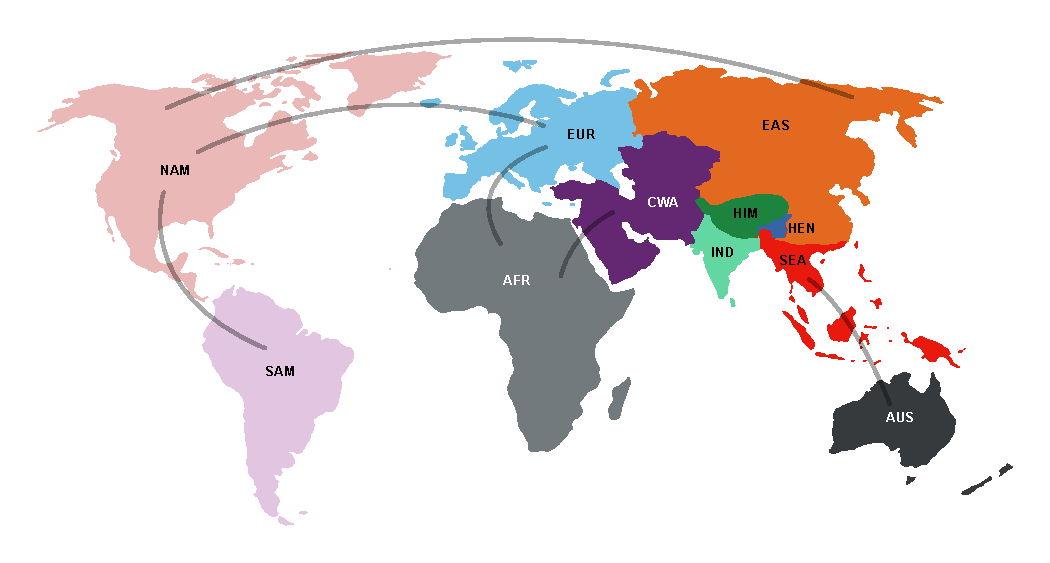
\includegraphics[width=.99\linewidth]{figures/regions.pdf}
\caption{Map of the 11 geographic regions used for ancestral range
  analyses in Lagrange.  HEN = Hengduan Mountains, HIM =
  Himalayas-QTP, EAS = temperate/boreal East Asia, SEA = Southeast
  Asia, CWA = Central/Western Asia, EUR = Europe, IND = India, AFR =
  Africa, NAM = North America, SAM = South America, AUS =
  Australasia. Lines and common borders indicate dispersal routes
  allowed in Lagrange.}
\label{fig:regions}
\end{figure}


\begin{figure}
  \caption{Reconstructions of ancestral geographic range (left) and
    net diversification rate (right) on the maximum clade credibility
    tree, with branch lengths set to posterior means, for each ingroup
    taxon (excluding \textit{Rhododendron}, shown as
    Fig.~4). Ancestral ranges are maximum-likelihood estimates at the
    start and end of each branch. Net diversification values are
    branch-segment means of the posterior distribution estimated by
    BAMM. Filled circles on the right indicate branches that appear in
    the 95\% credible set of distinct shift configurations, with the
    size and label of a circle indicating the cumulative probability
    of the branch over all configurations in the credible set. On the
    left, the marginal odds ratio for a shift in diversification
    regime along a branch is drawn for branches where the ratio
    exceeds 20. Geographic regions are coded as follows: HEN, Hengduan
    Mountains; HIM, Himalayas-QTP; EAS, temperate-boreal East Asia;
    SEA, Southeast Asia; CWA, central/western Asia; EUR, Europe; IND,
    India; AFR, Africa; NAM, North America; SAM, South America; AUS,
    Australasia.}
  \label{fig:ancranges}
\end{figure}

\addtocounter{figure}{-1}

\begin{figure}
\begin{subfigure}{\textwidth}
\centering
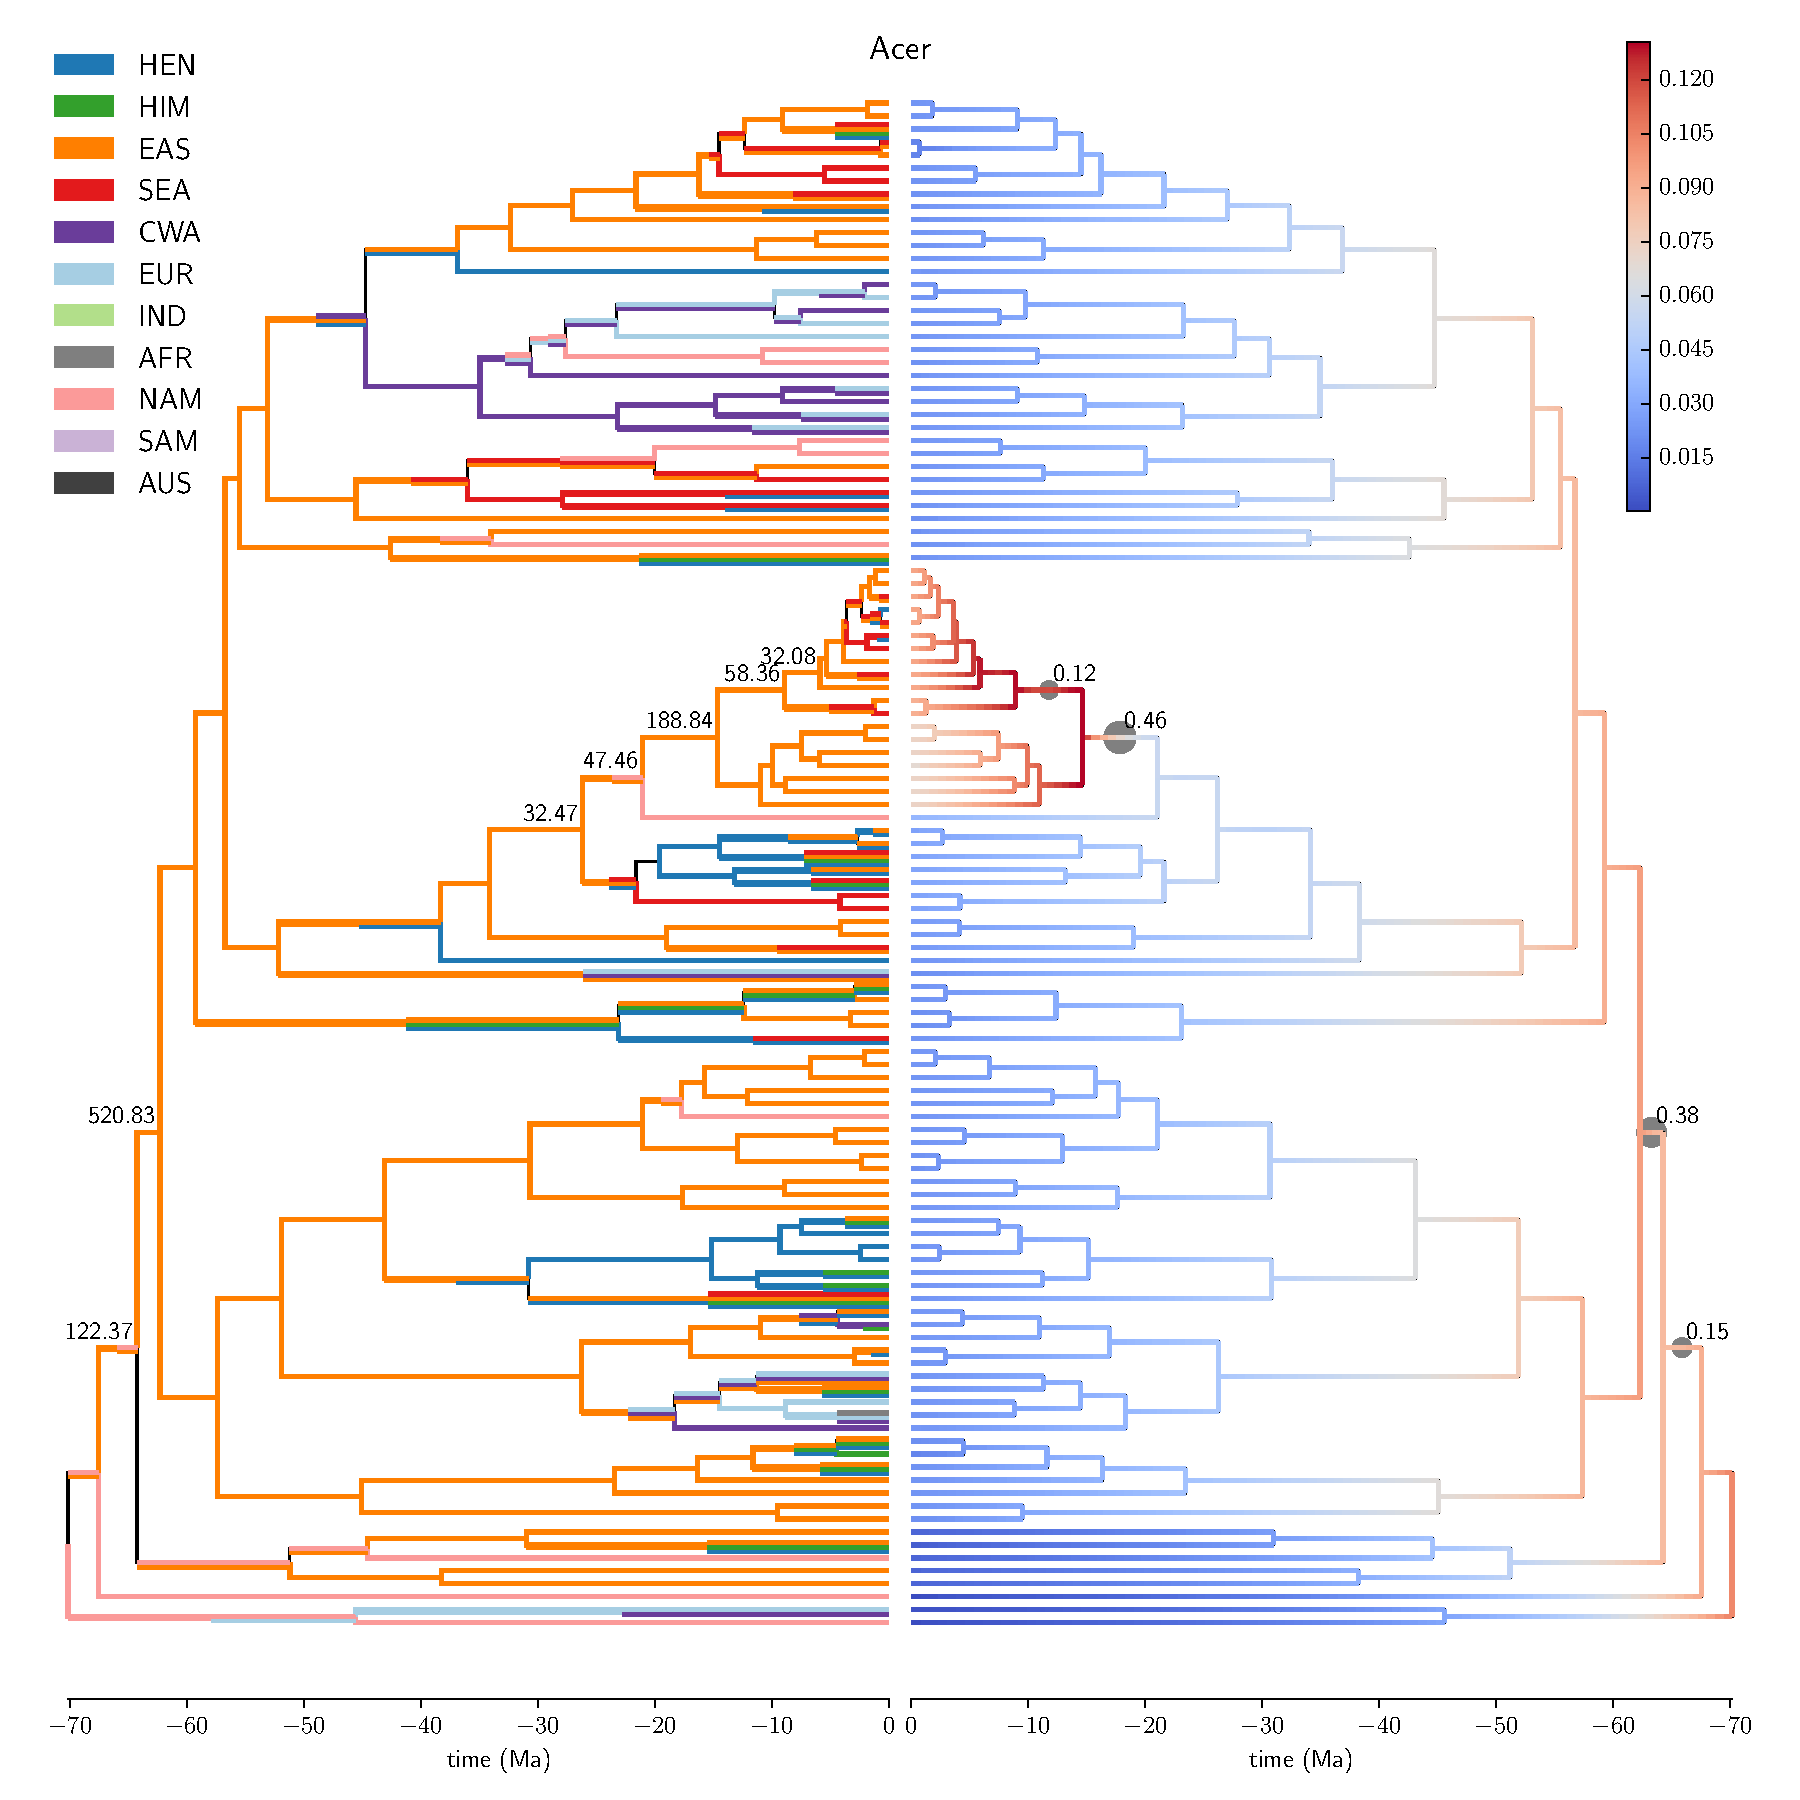
\includegraphics[width=.99\linewidth]{figures/Acer-supfig.pdf}
\label{fig:acer}
\caption{\textit{Acer}}
\end{subfigure}
\end{figure}

\begin{figure}
  \ContinuedFloat
\begin{subfigure}{\textwidth}
\centering
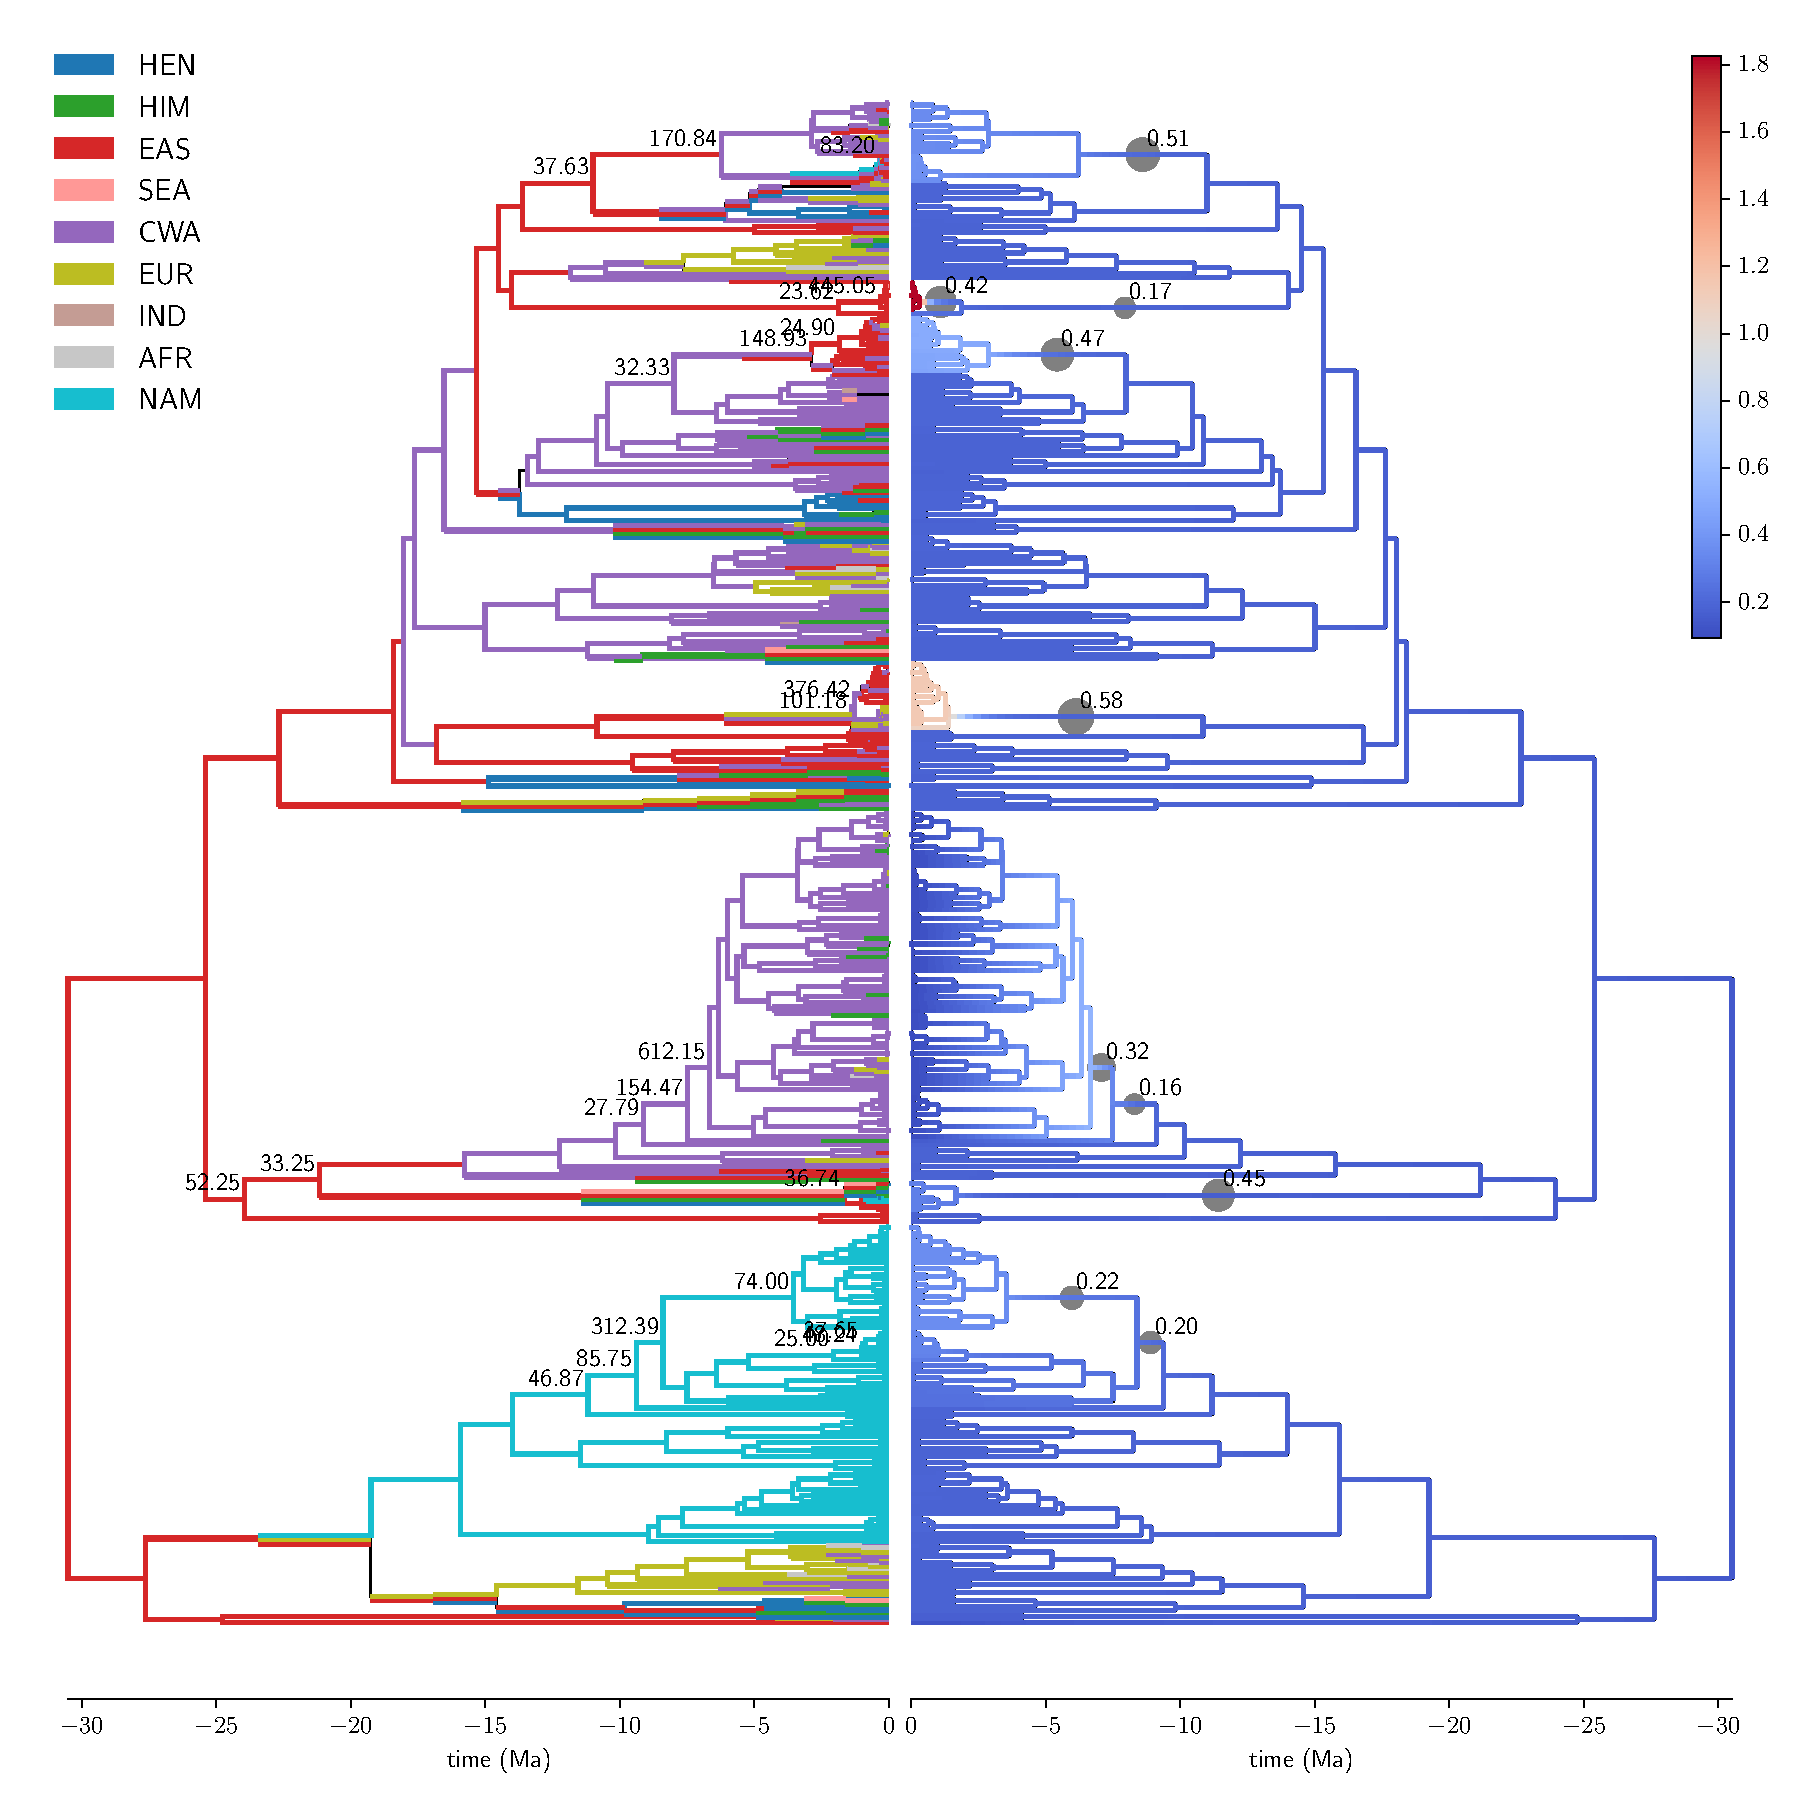
\includegraphics[width=.99\linewidth]{figures/Allium-supfig.pdf}
\label{fig:allium}
\caption{\textit{Allium}}
\end{subfigure}
\end{figure}

\begin{figure}
  \ContinuedFloat
\begin{subfigure}{\textwidth}
\centering
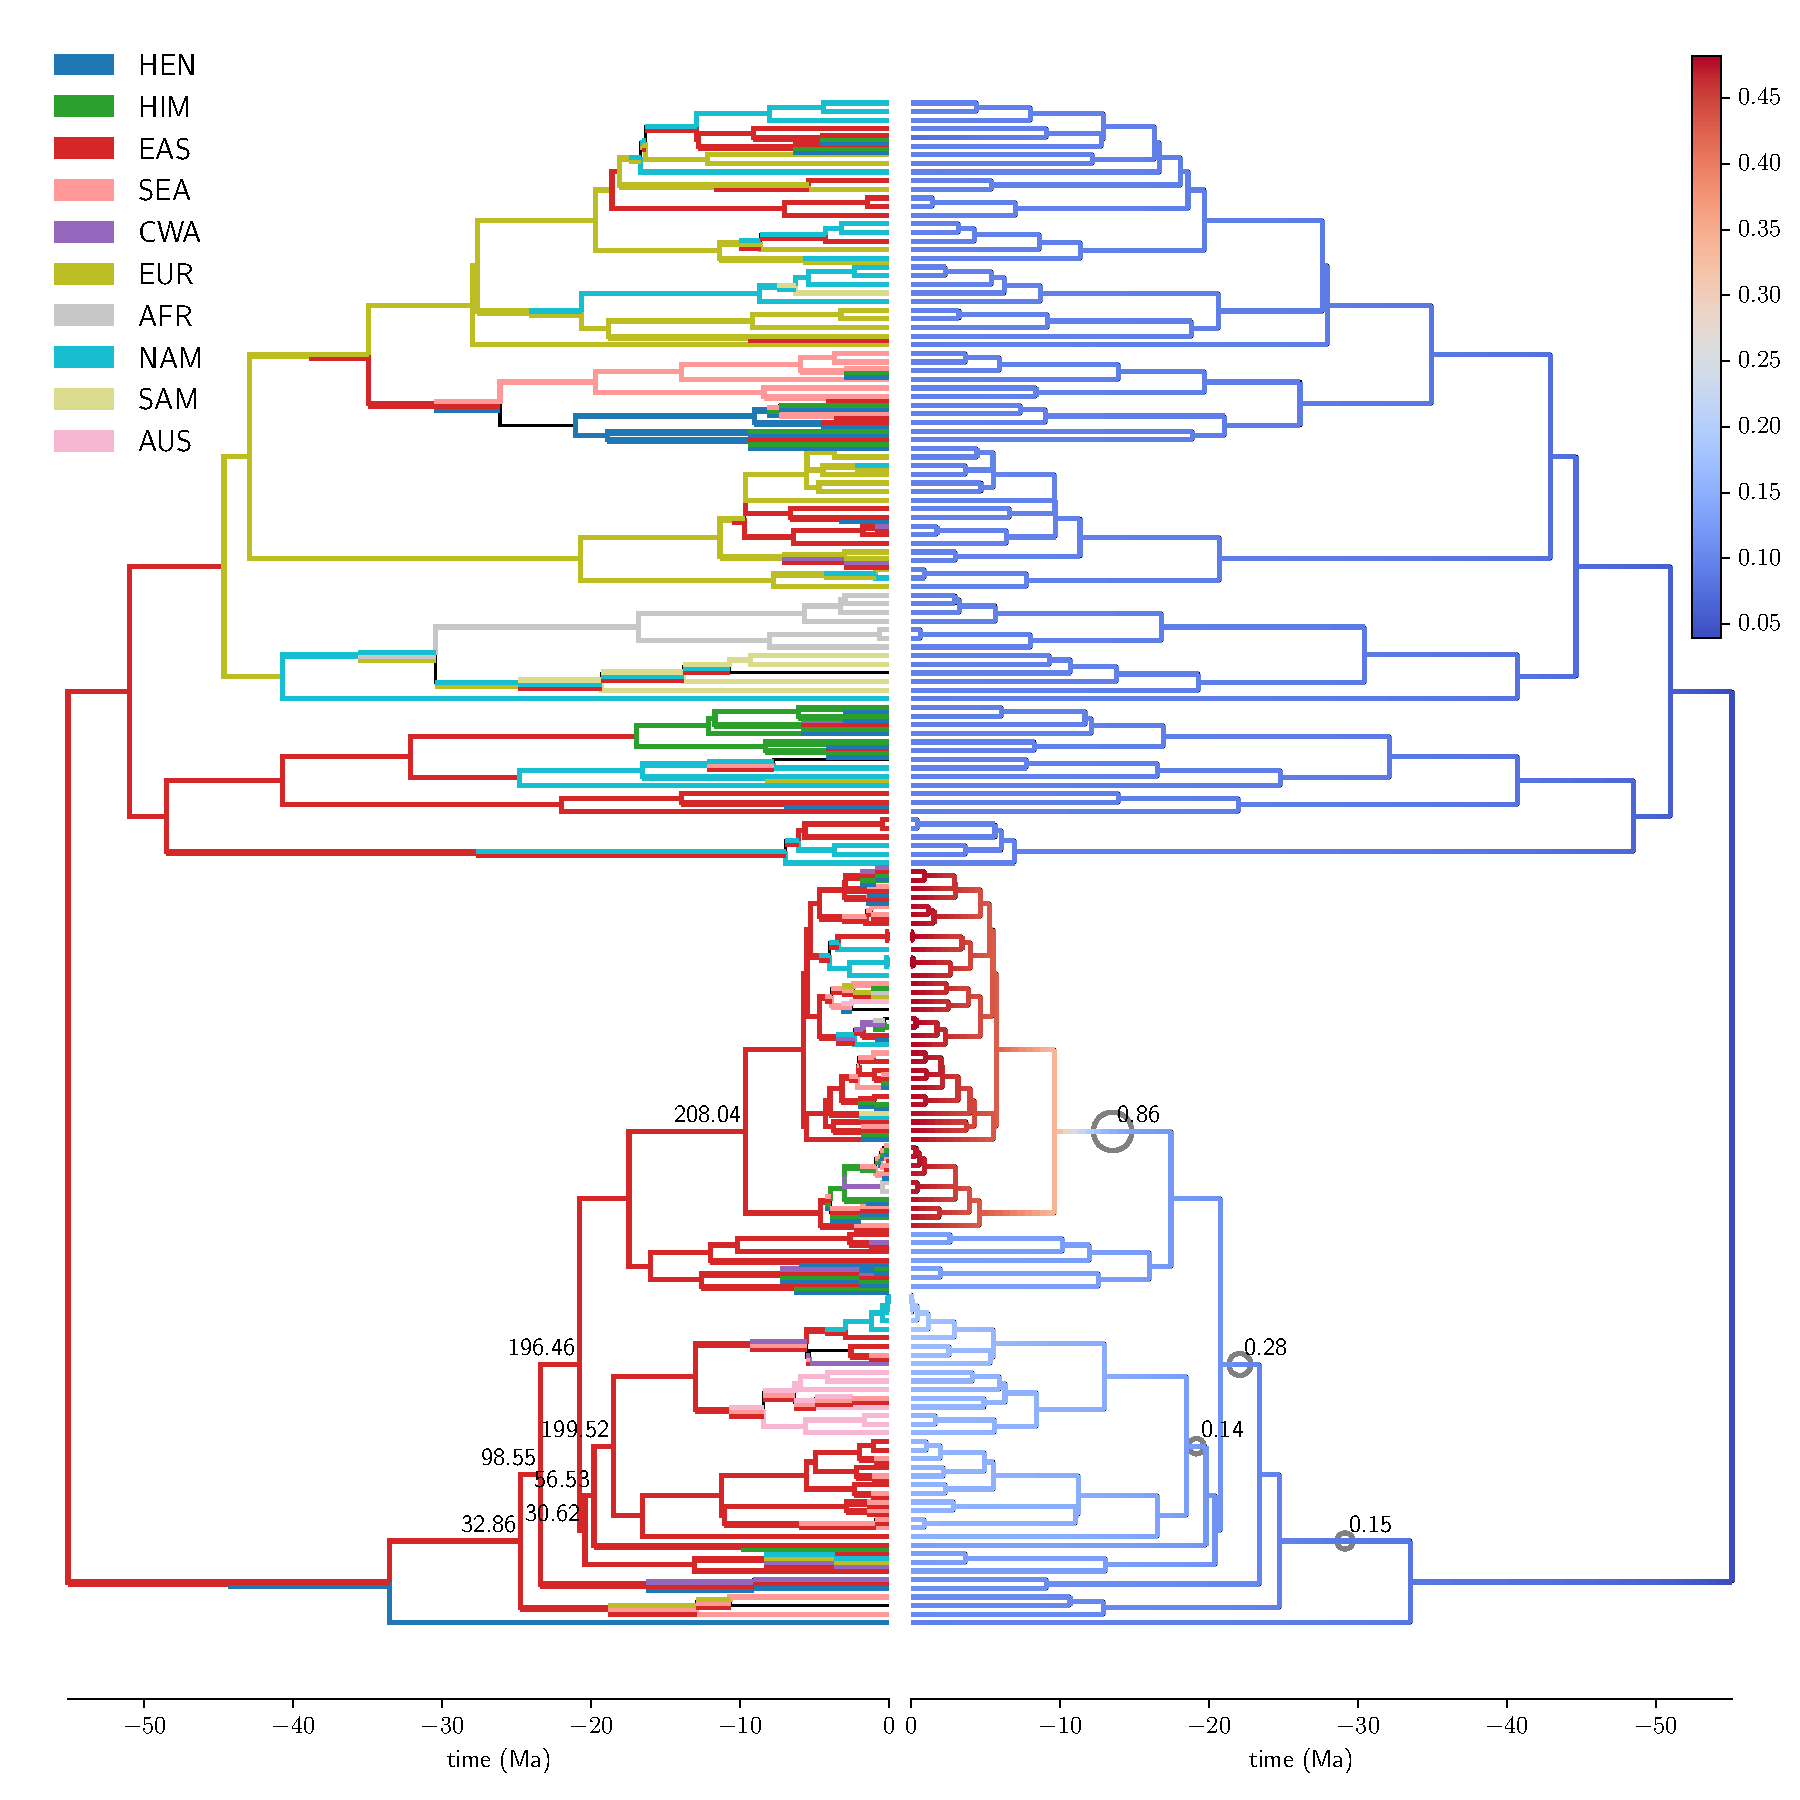
\includegraphics[width=.99\linewidth]{figures/Clematis-supfig.pdf}
\label{fig:allium}
\caption{Clematidinae+Anemoninae}
\end{subfigure}
\end{figure}

\begin{figure}
  \ContinuedFloat
\begin{subfigure}{\textwidth}
\centering
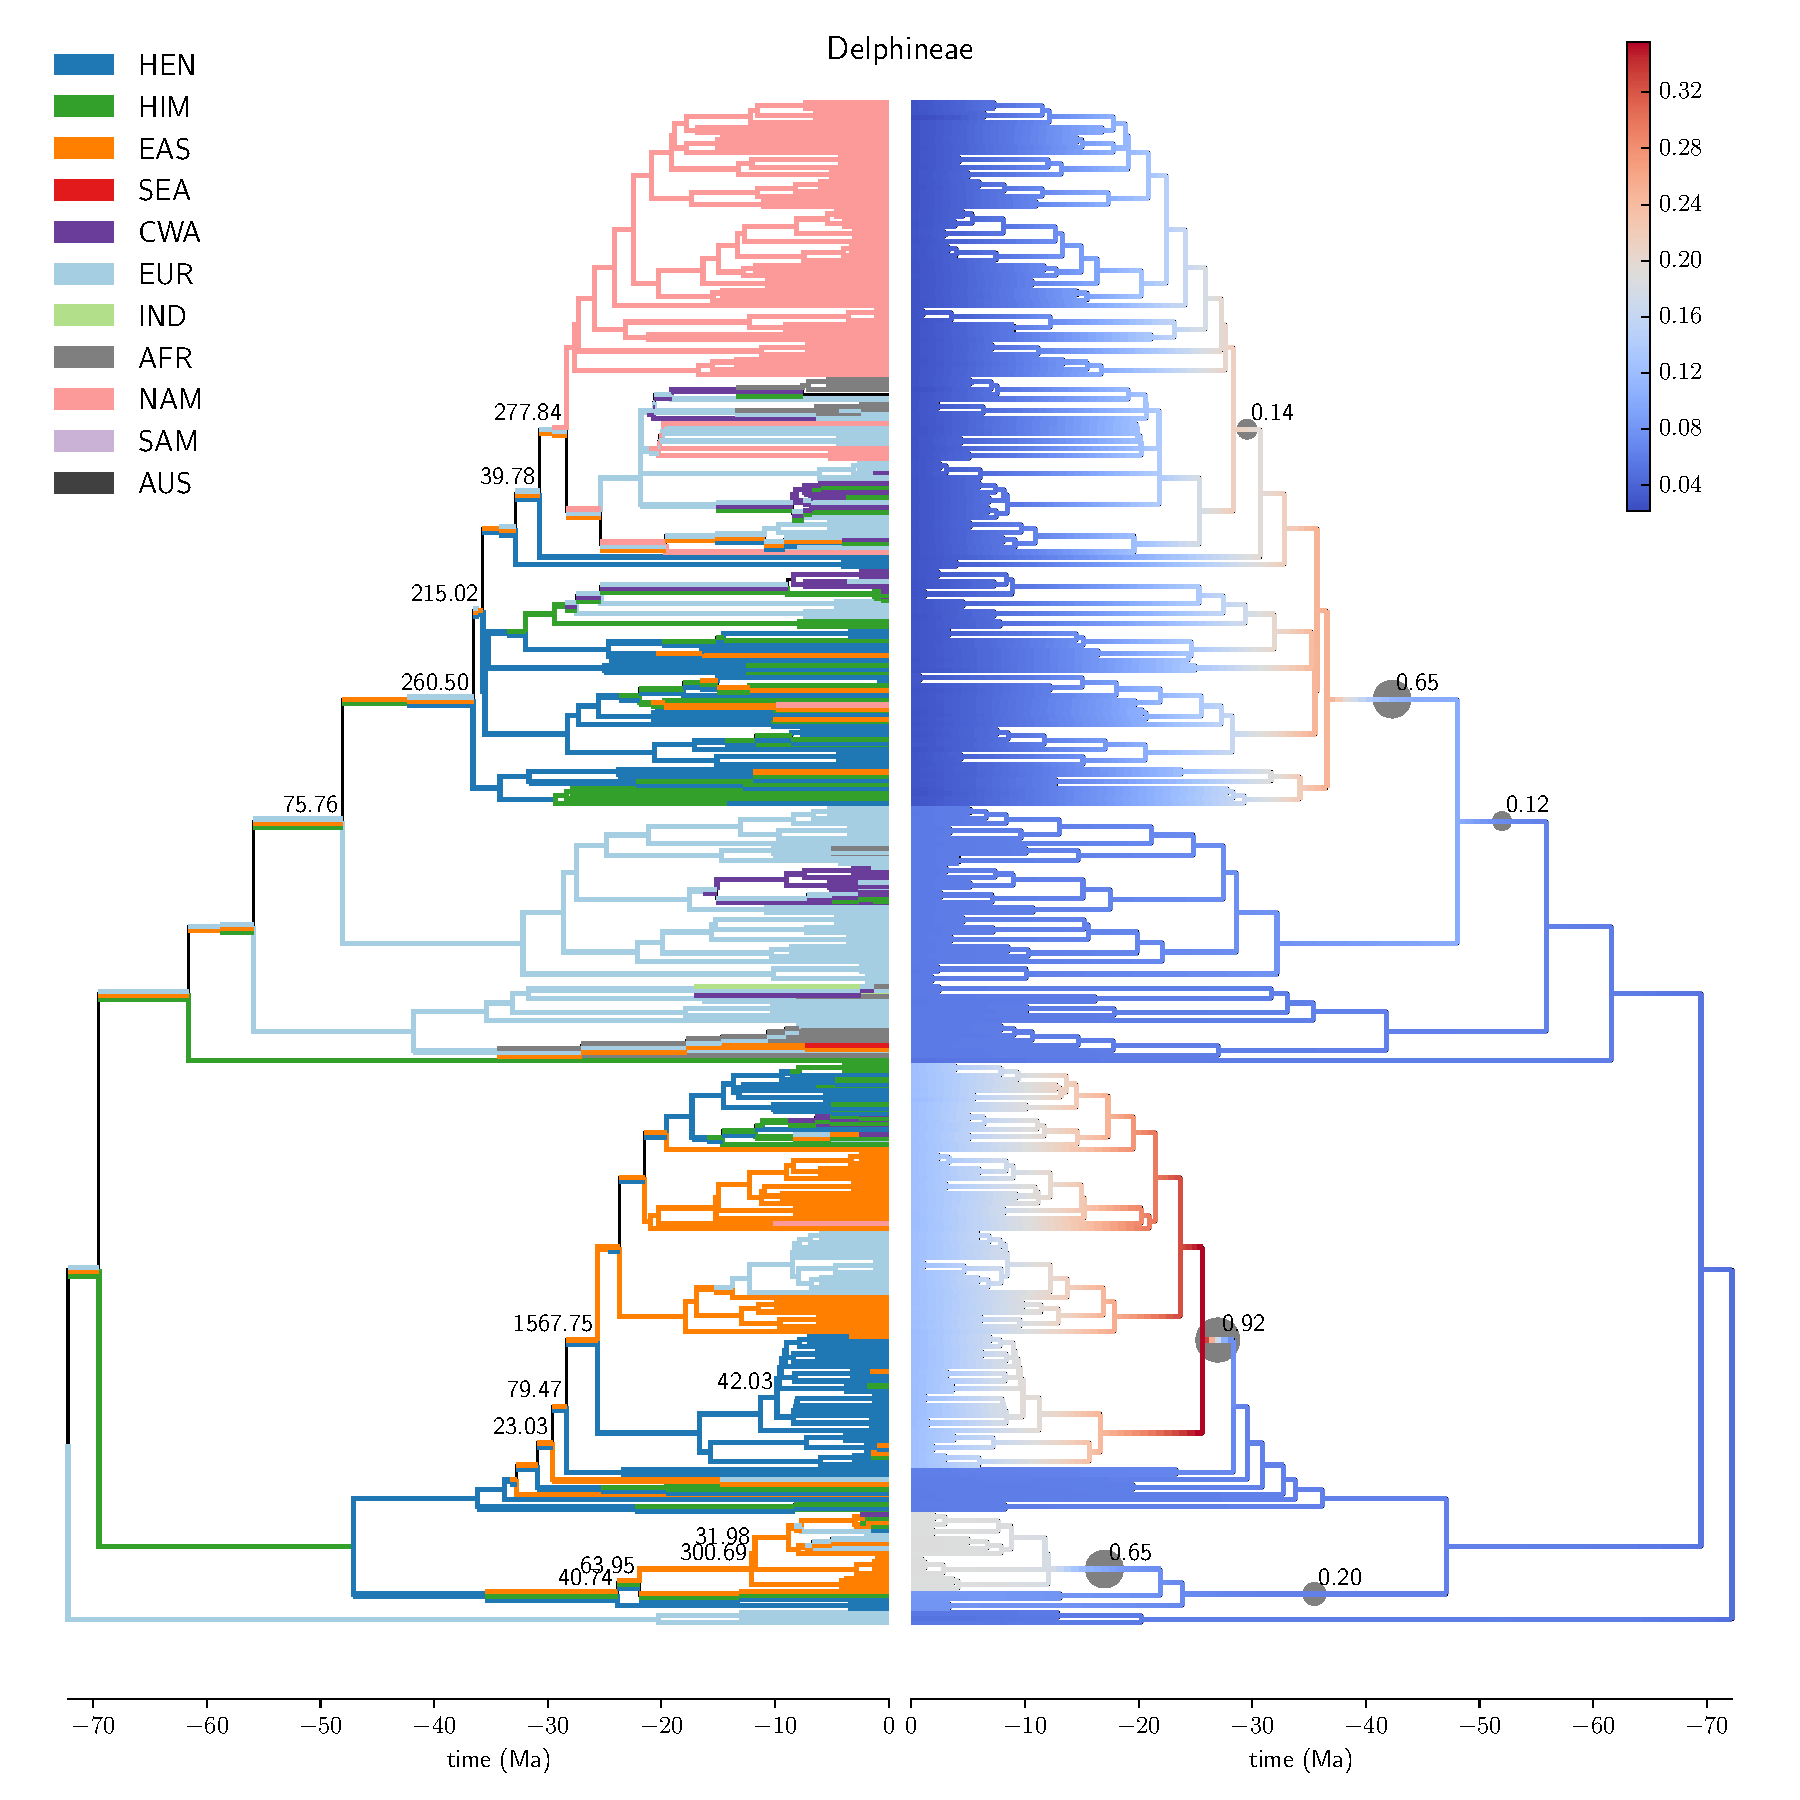
\includegraphics[width=.99\linewidth]{figures/Delphineae-supfig.pdf}
\label{fig:allium}
\caption{Delphineae}
\end{subfigure}
\end{figure}

\begin{figure}
  \ContinuedFloat
\begin{subfigure}{\textwidth}
\centering
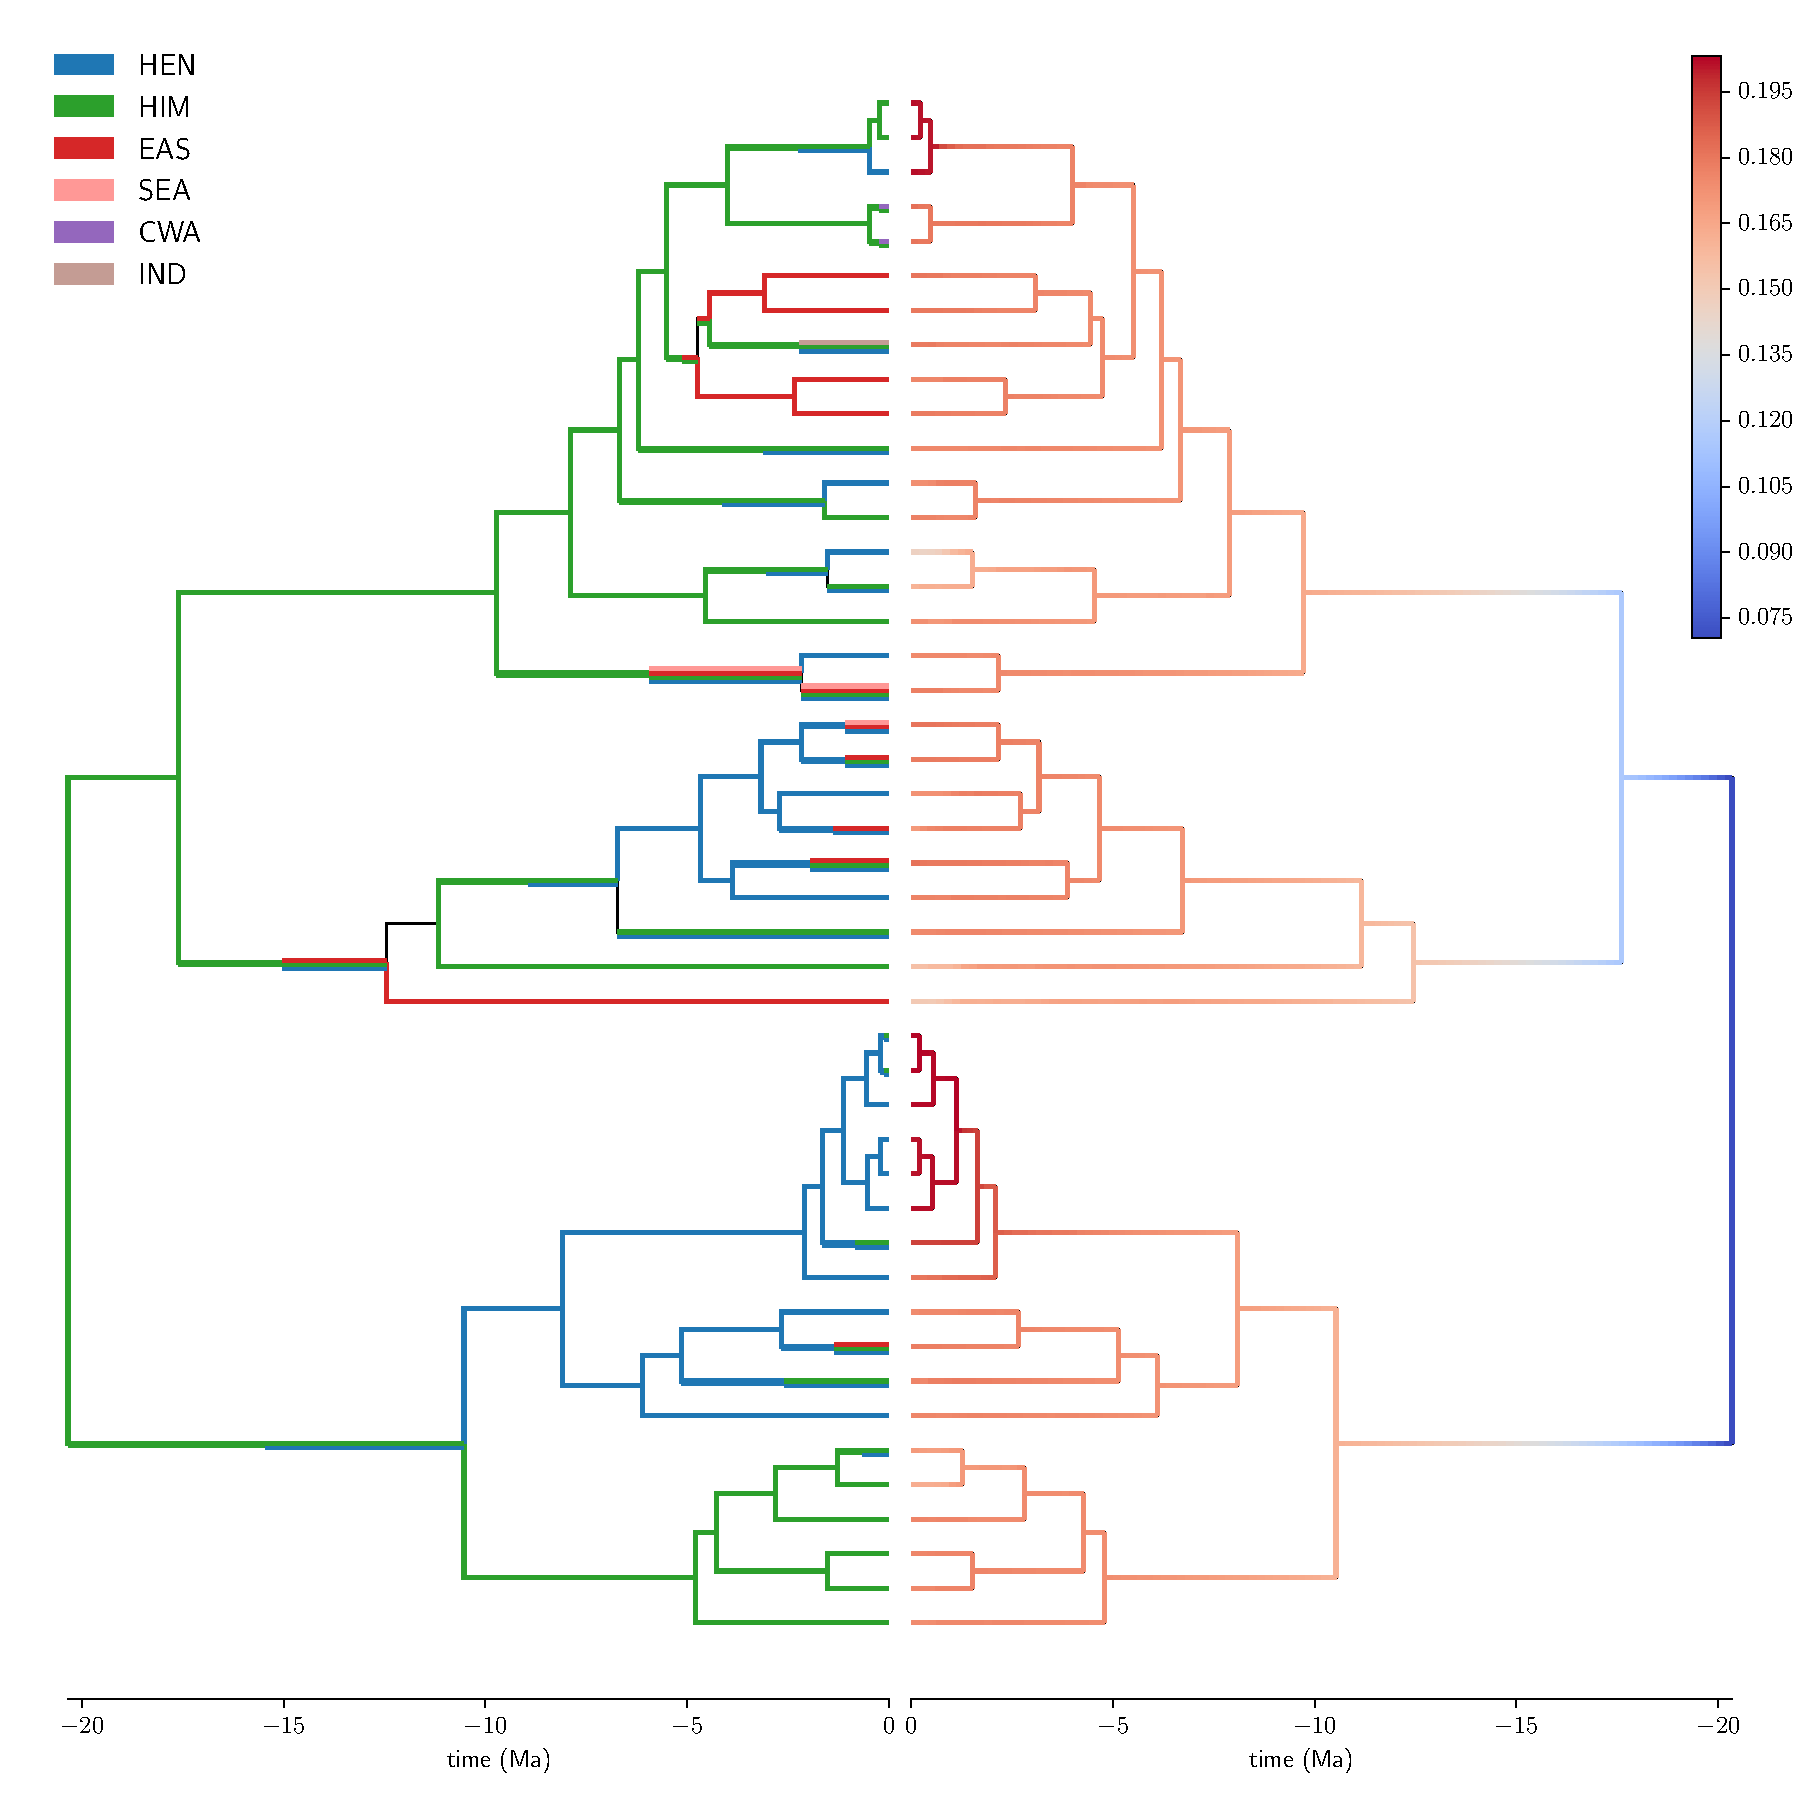
\includegraphics[width=.99\linewidth]{figures/Cyananthus-supfig.pdf}
\label{fig:allium}
\caption{\textit{Cyananthus}}
\end{subfigure}
\end{figure}

\begin{figure}
  \ContinuedFloat
\begin{subfigure}{\textwidth}
\centering
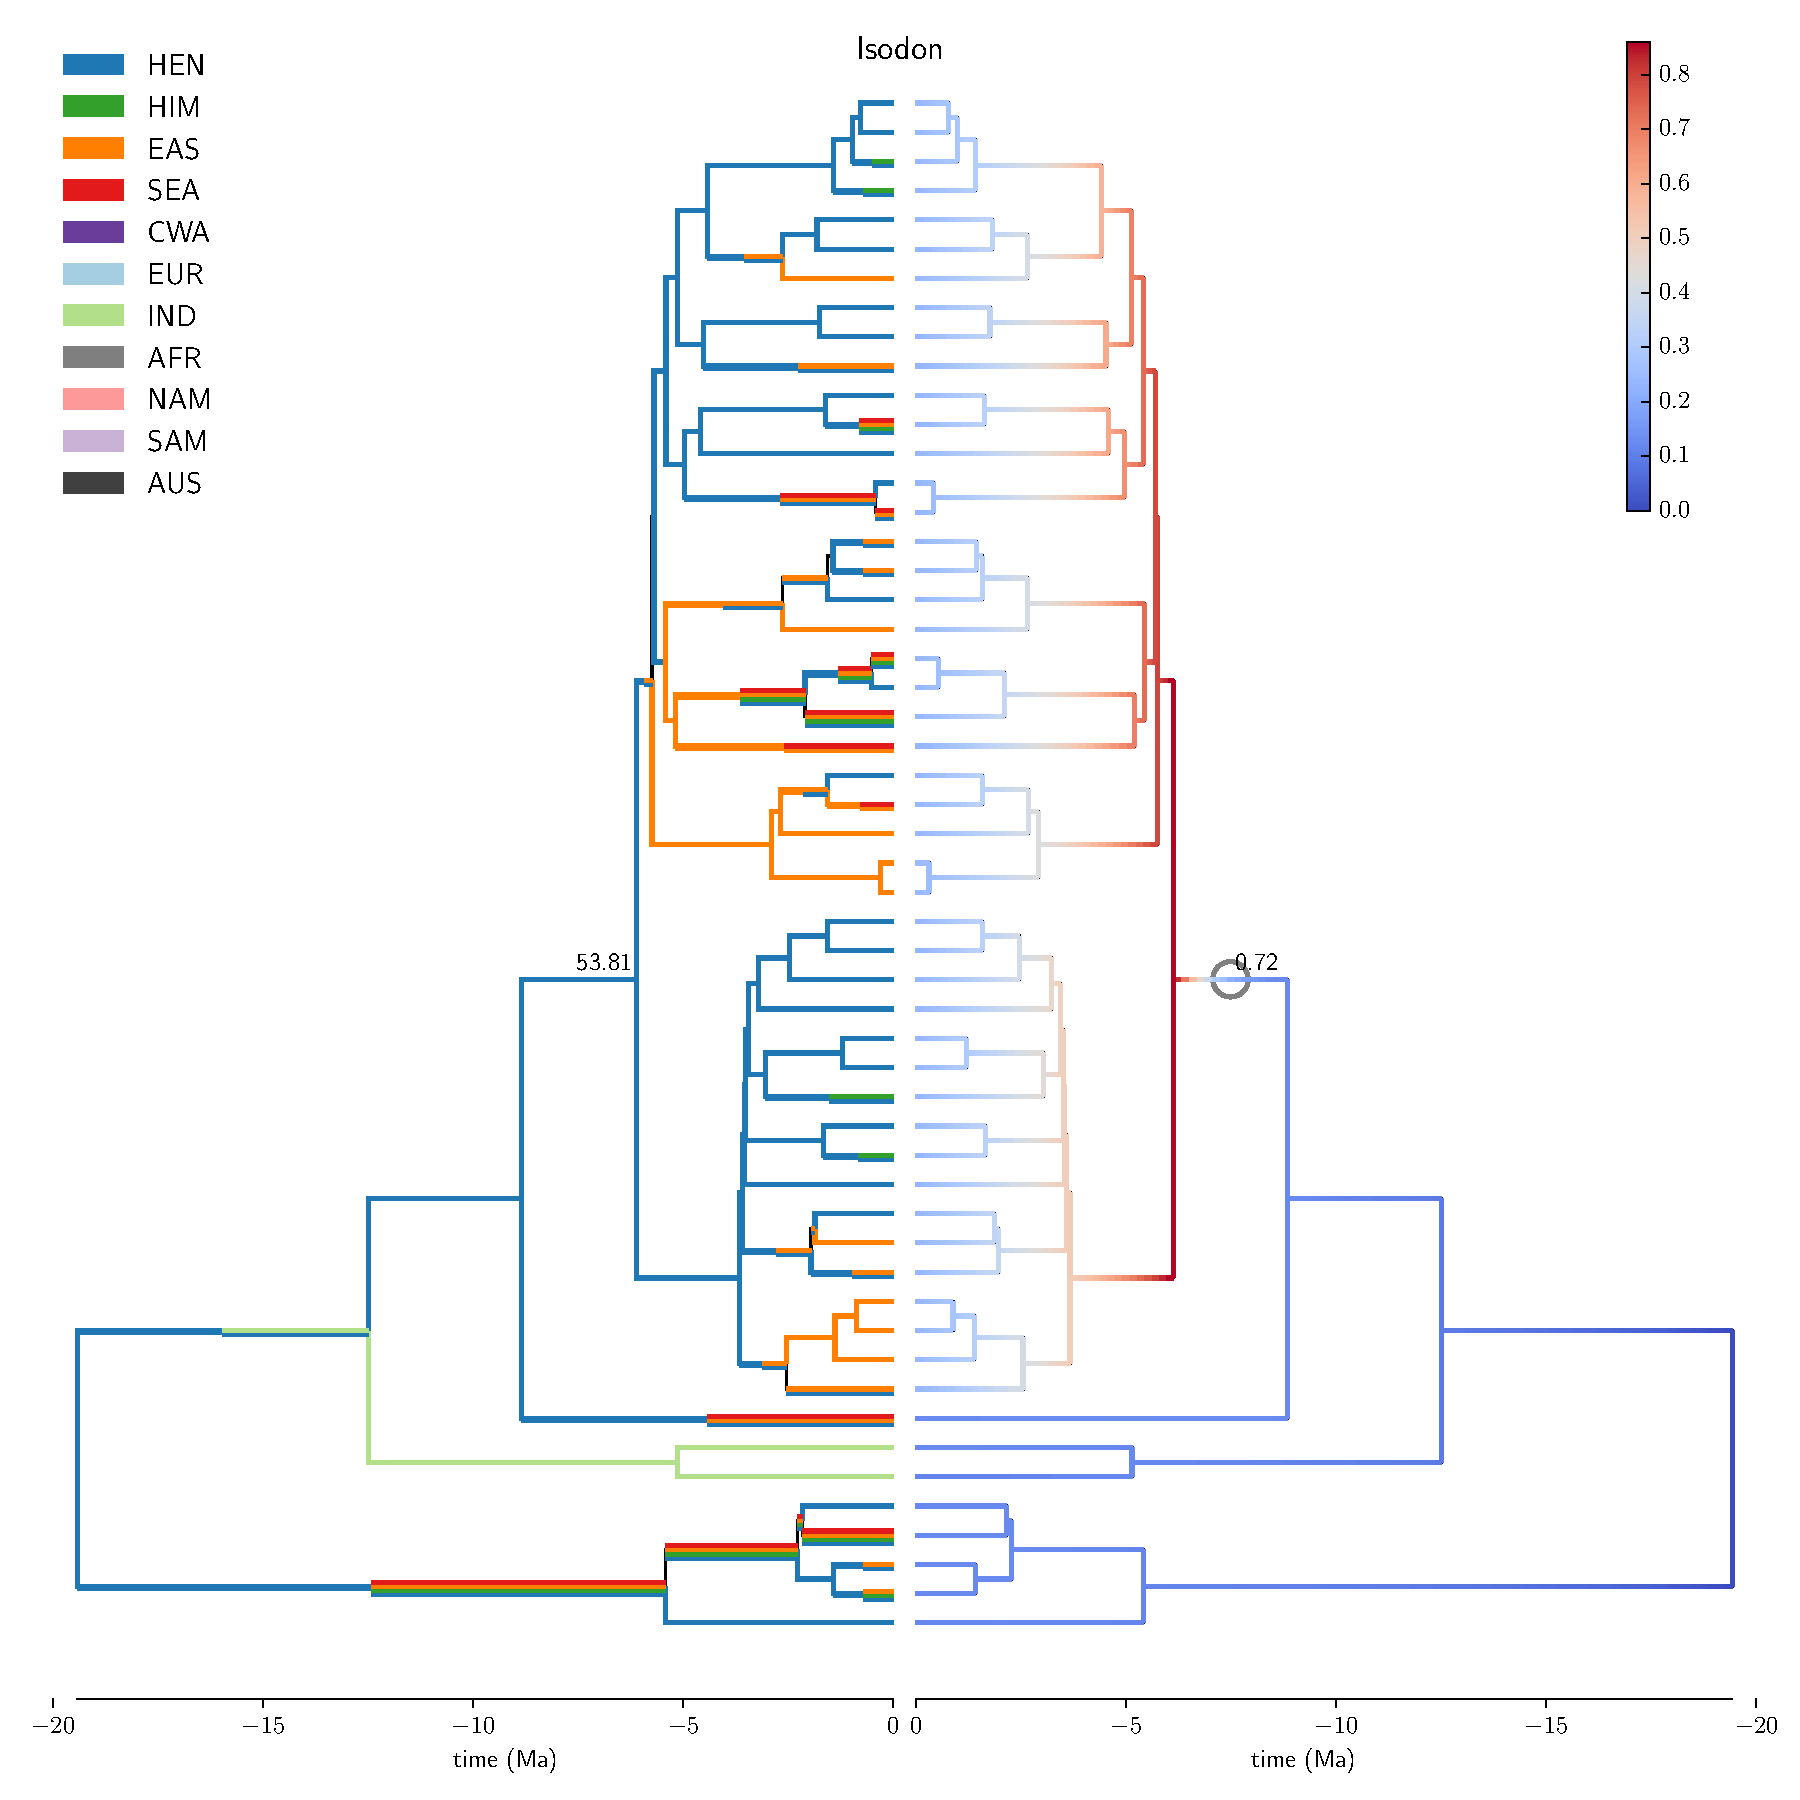
\includegraphics[width=.99\linewidth]{figures/Isodon-supfig.pdf}
\label{fig:allium}
\caption{\textit{Isodon}}
\end{subfigure}
\end{figure}

\begin{figure}
  \ContinuedFloat
\begin{subfigure}{\textwidth}
\centering
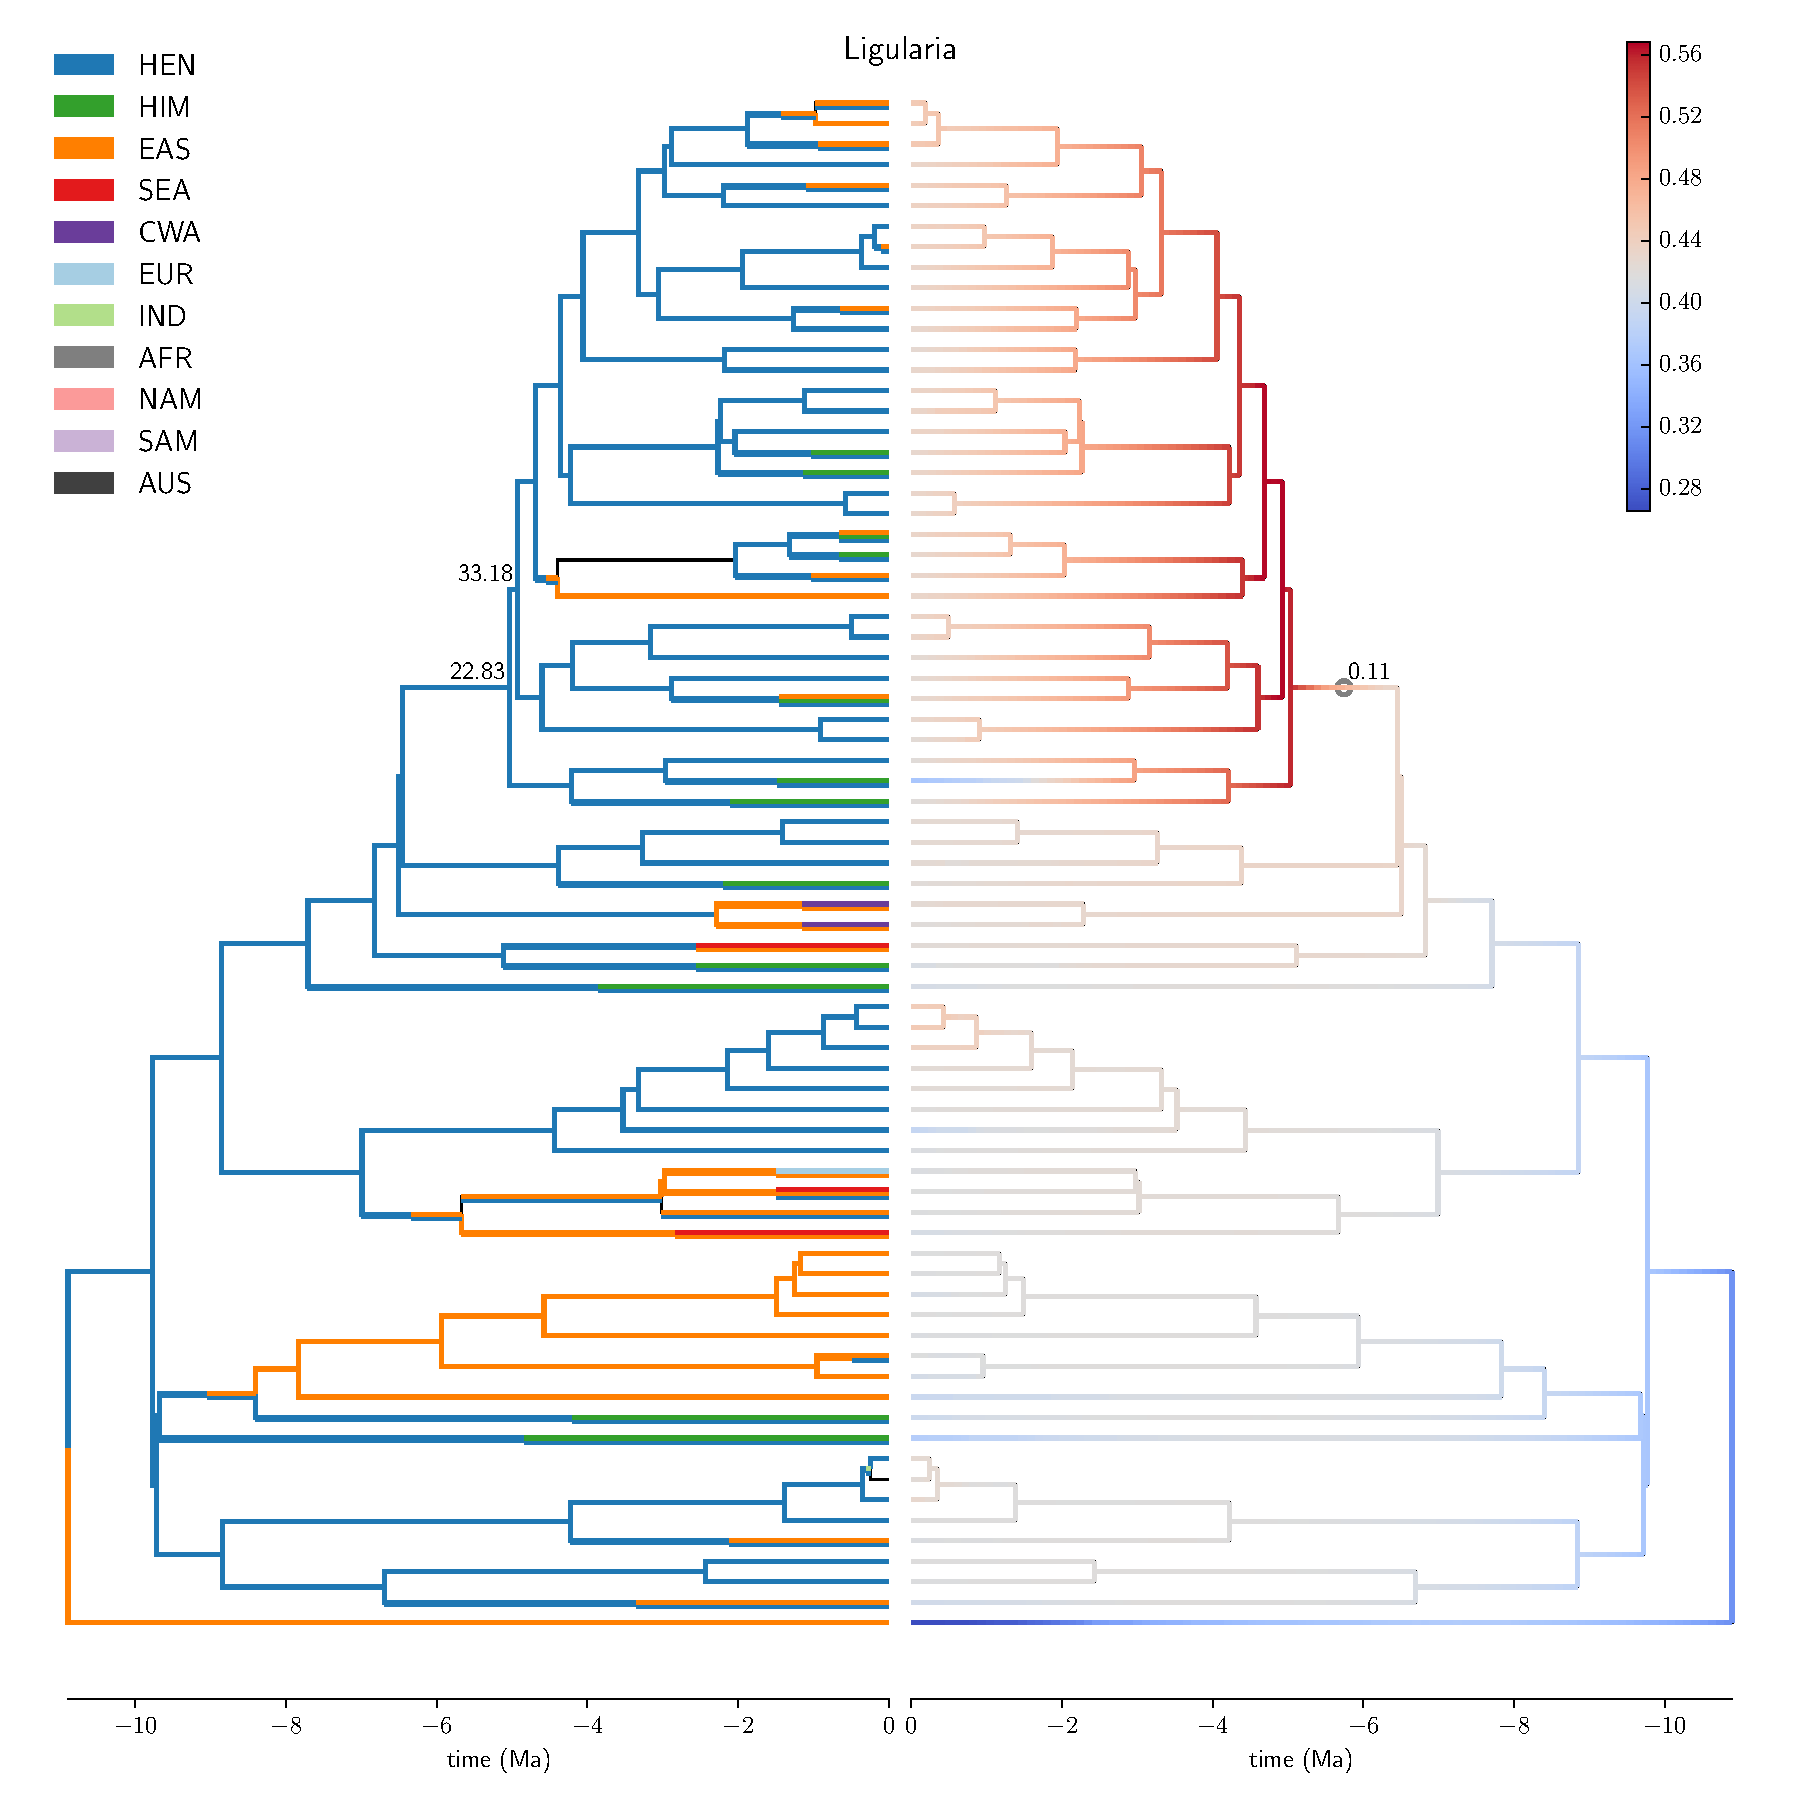
\includegraphics[width=.99\linewidth]{figures/Ligularia-supfig.pdf}
\label{fig:allium}
\caption{\textit{Ligularia-Cremanthodium-Parasenecio} complex}
\end{subfigure}
\end{figure}

\begin{figure}
  \ContinuedFloat
\begin{subfigure}{\textwidth}
\centering
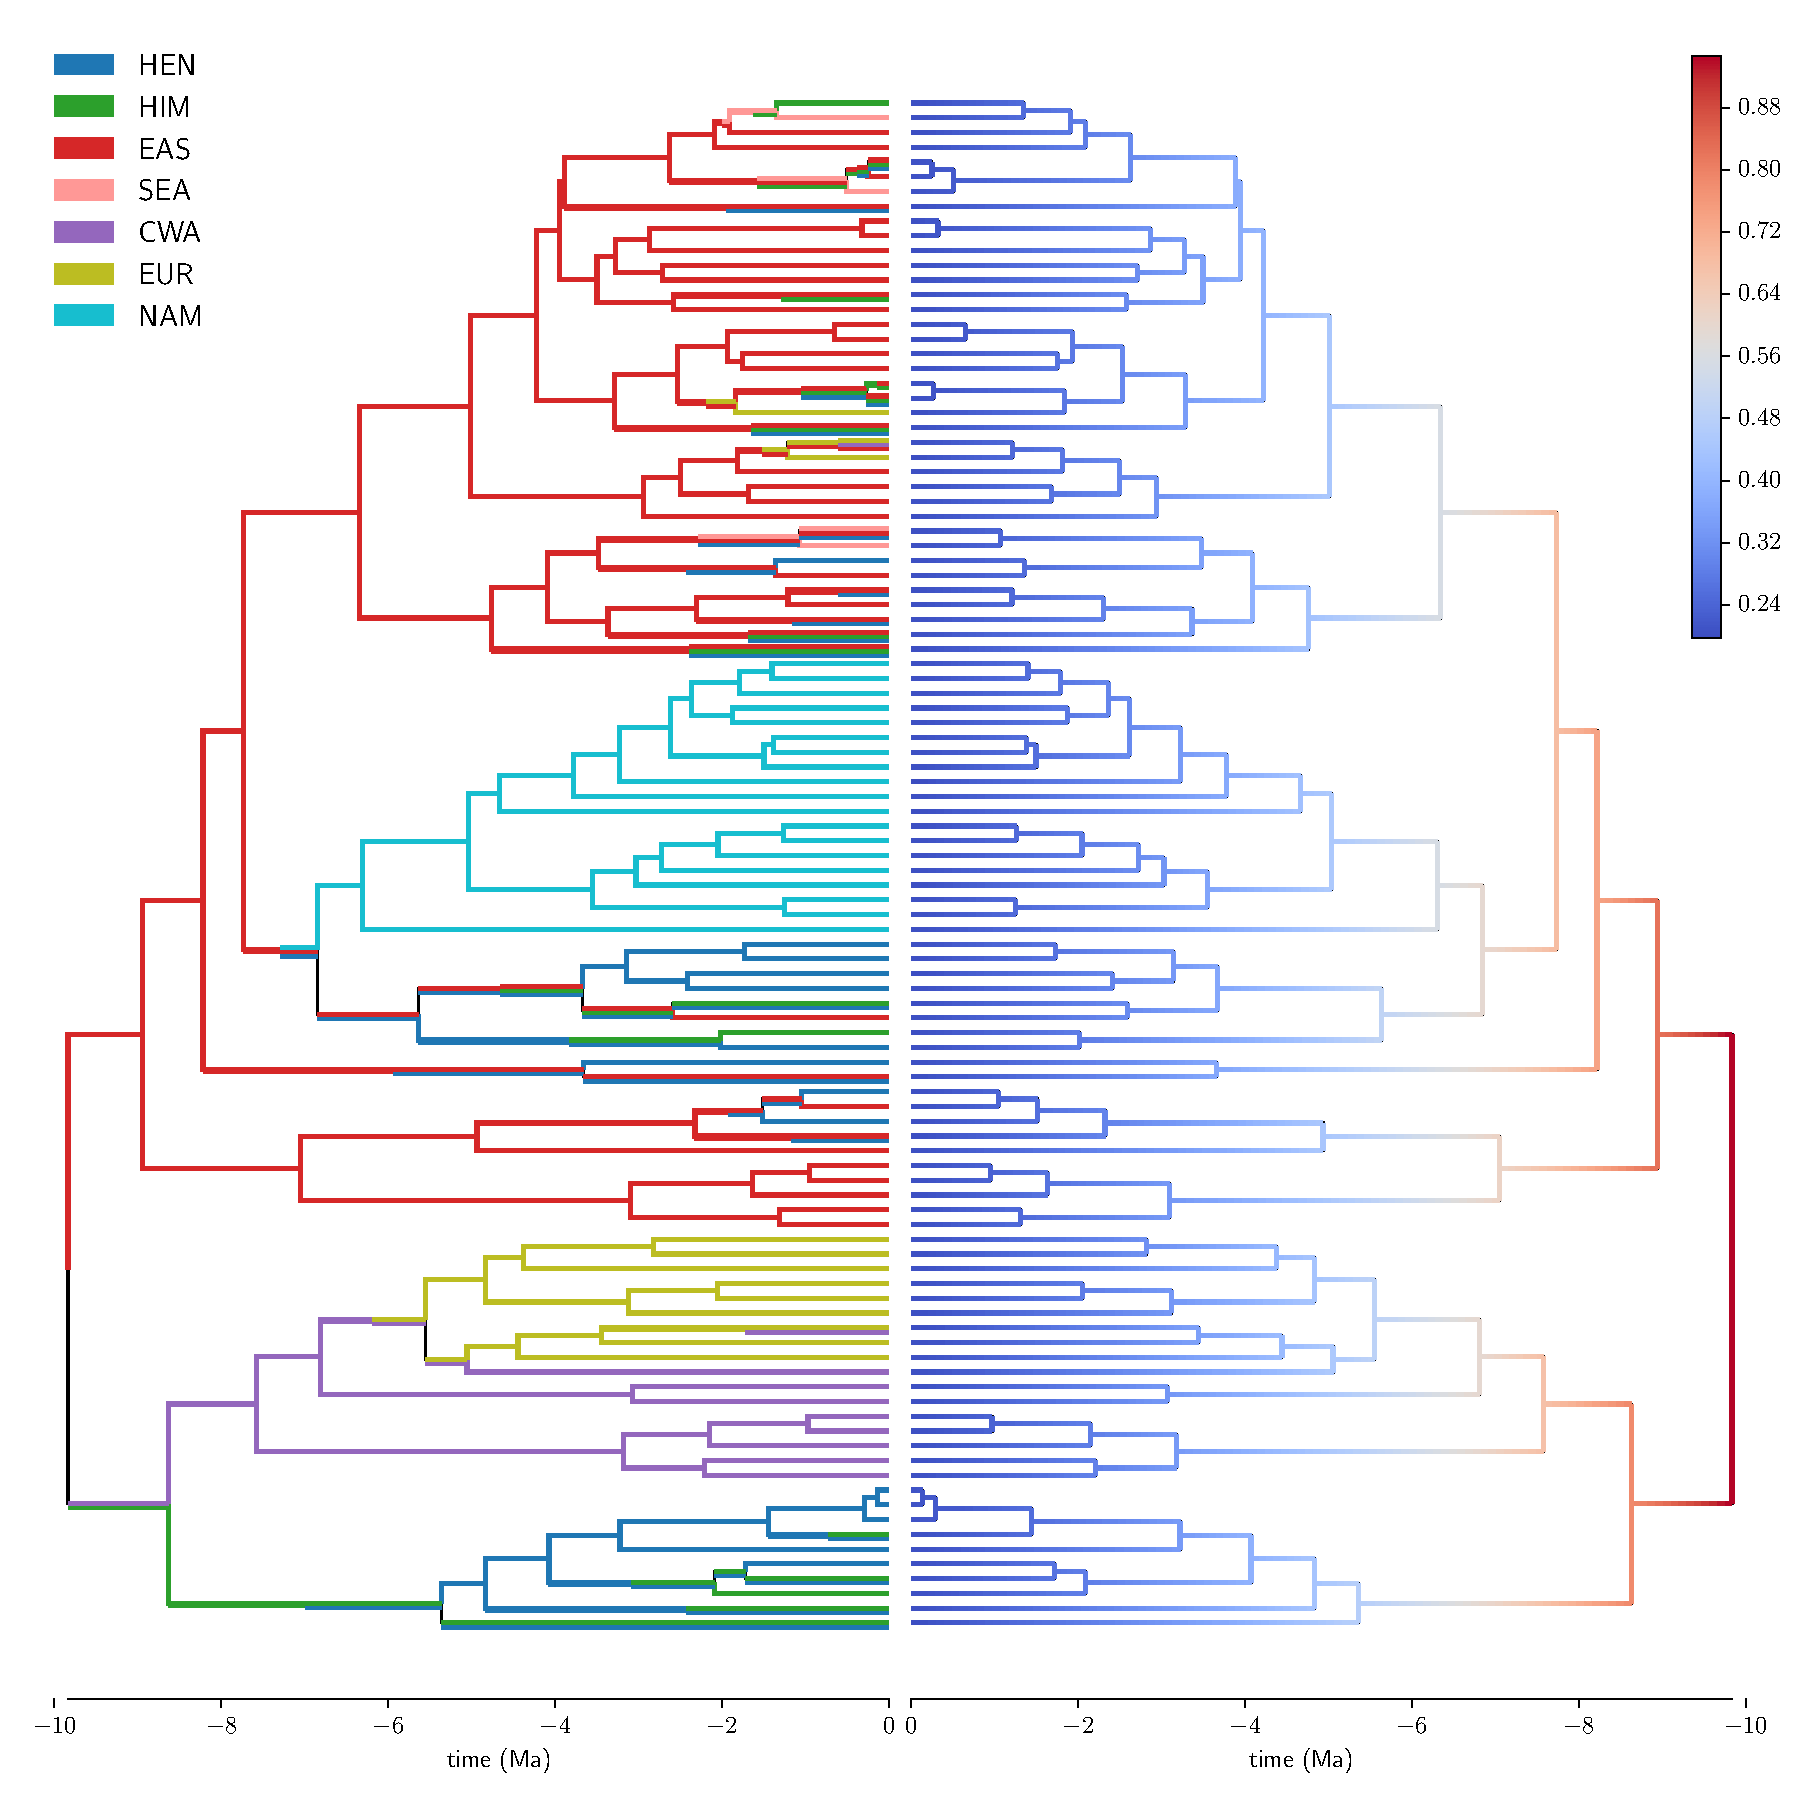
\includegraphics[width=.99\linewidth]{figures/Lilium-supfig.pdf}
\label{fig:allium}
\caption{\textit{Lilium} (including \textit{Nomocharis})}
\end{subfigure}
\end{figure}

\begin{figure}
  \ContinuedFloat
\begin{subfigure}{\textwidth}
\centering
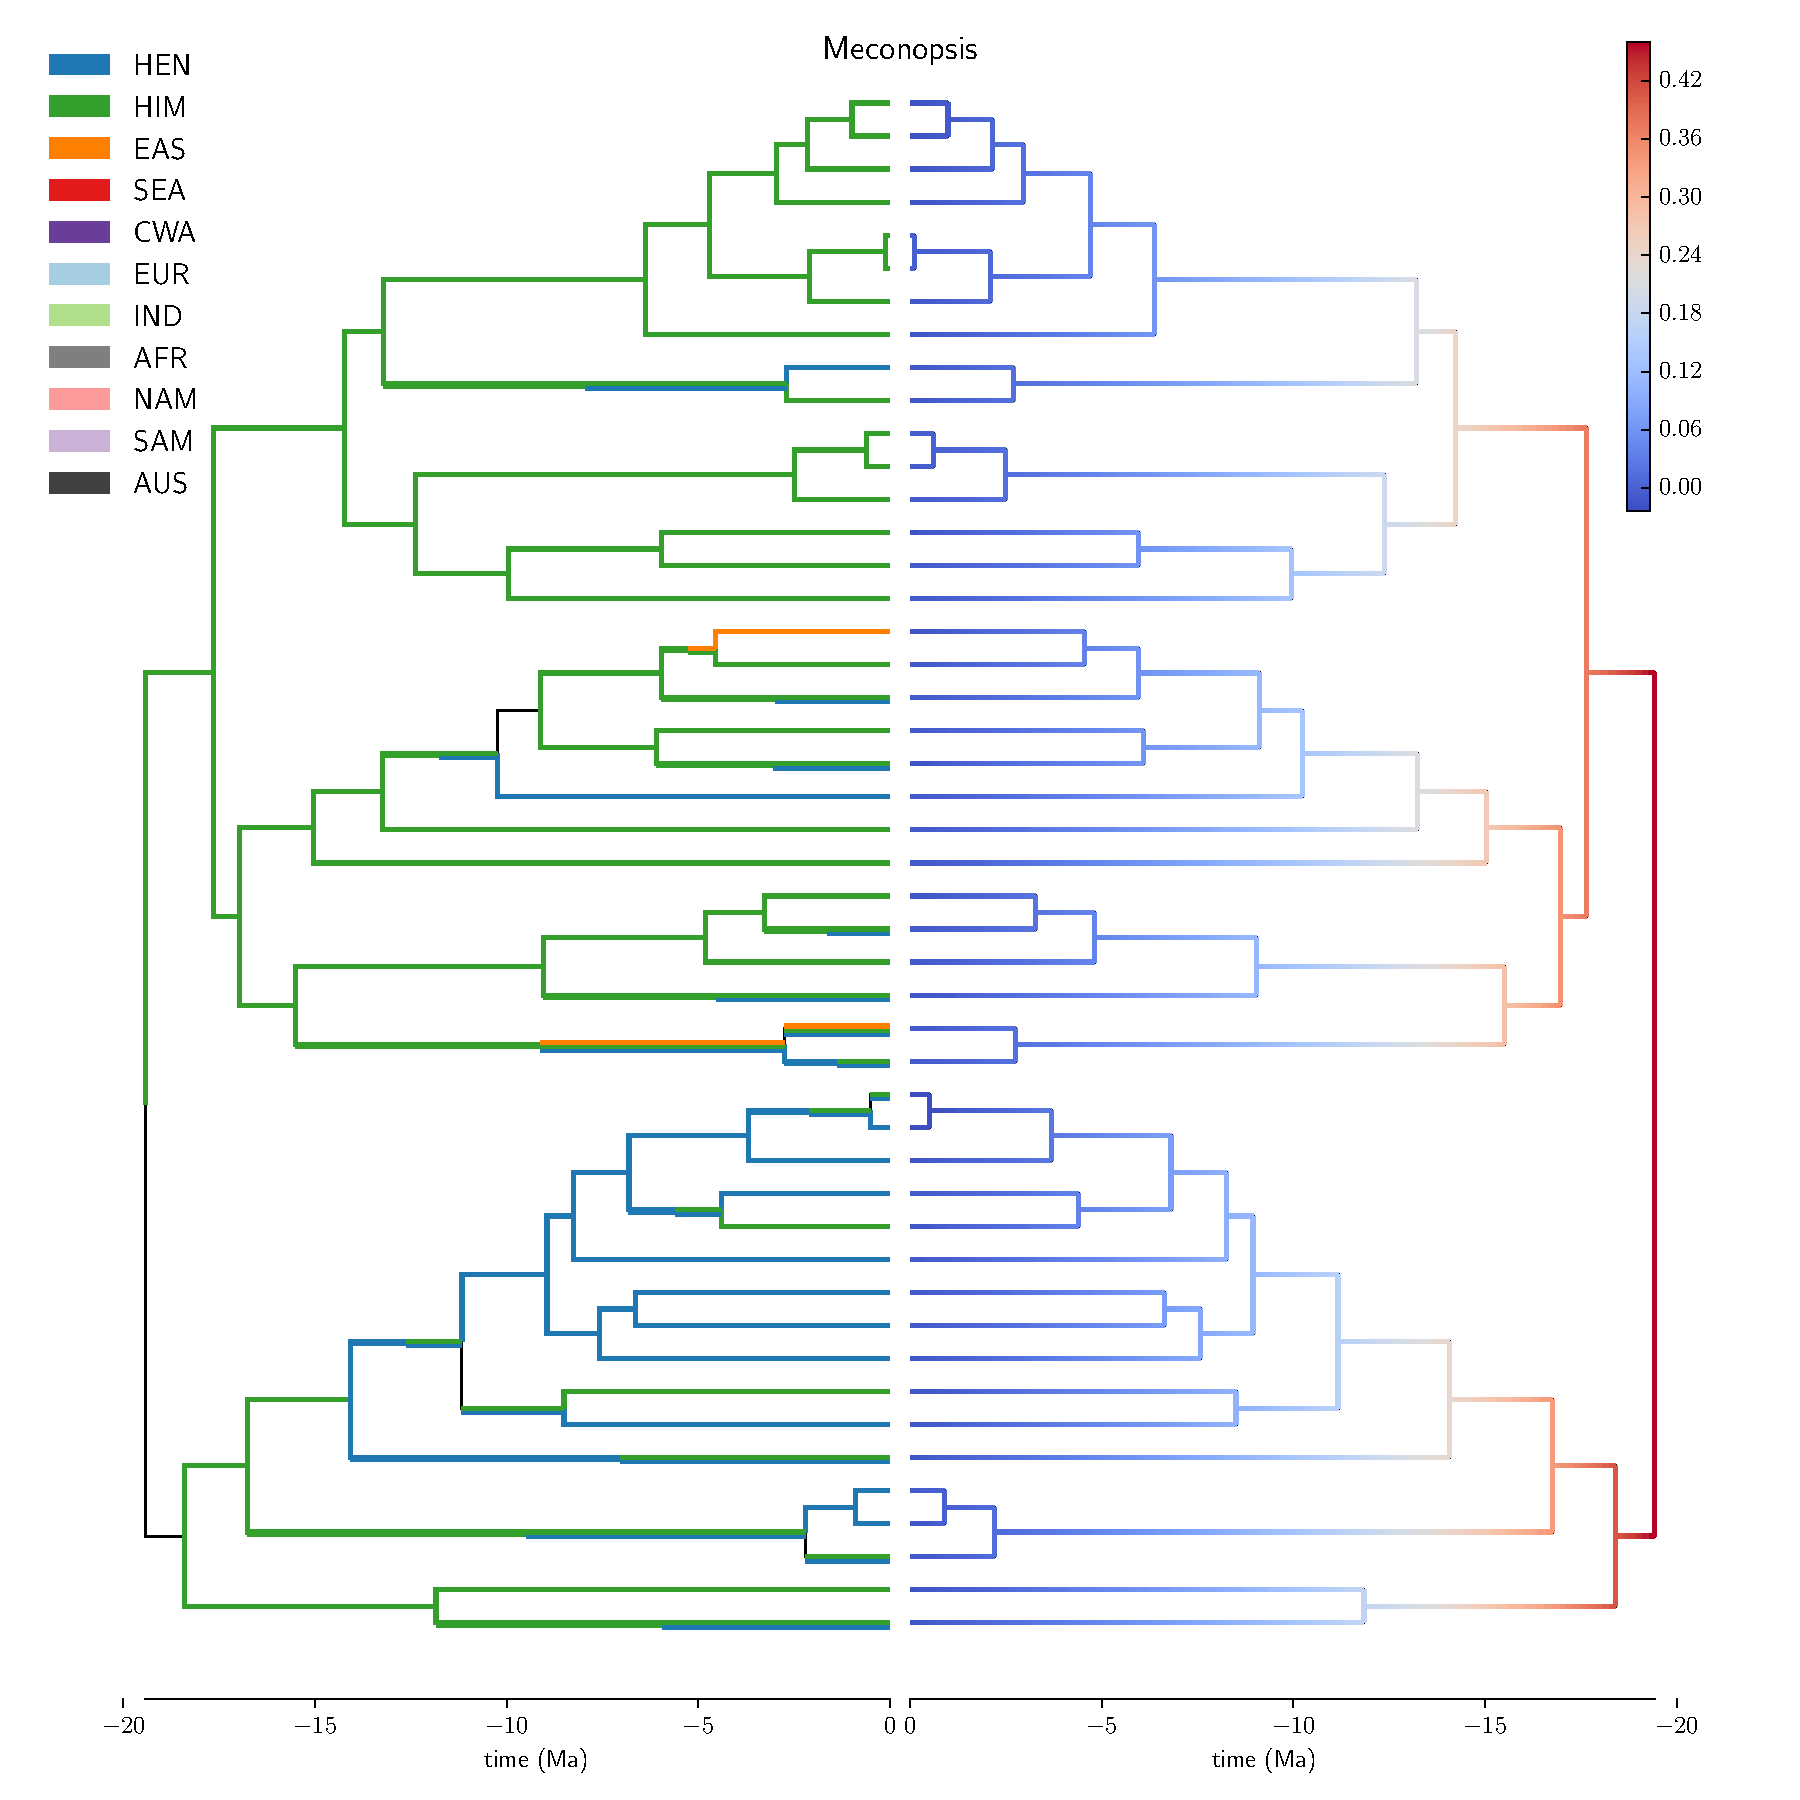
\includegraphics[width=.99\linewidth]{figures/Meconopsis-supfig.pdf}
\label{fig:allium}
\caption{\textit{Meconopsis}}
\end{subfigure}
\end{figure}

\begin{figure}
  \ContinuedFloat
\begin{subfigure}{\textwidth}
\centering
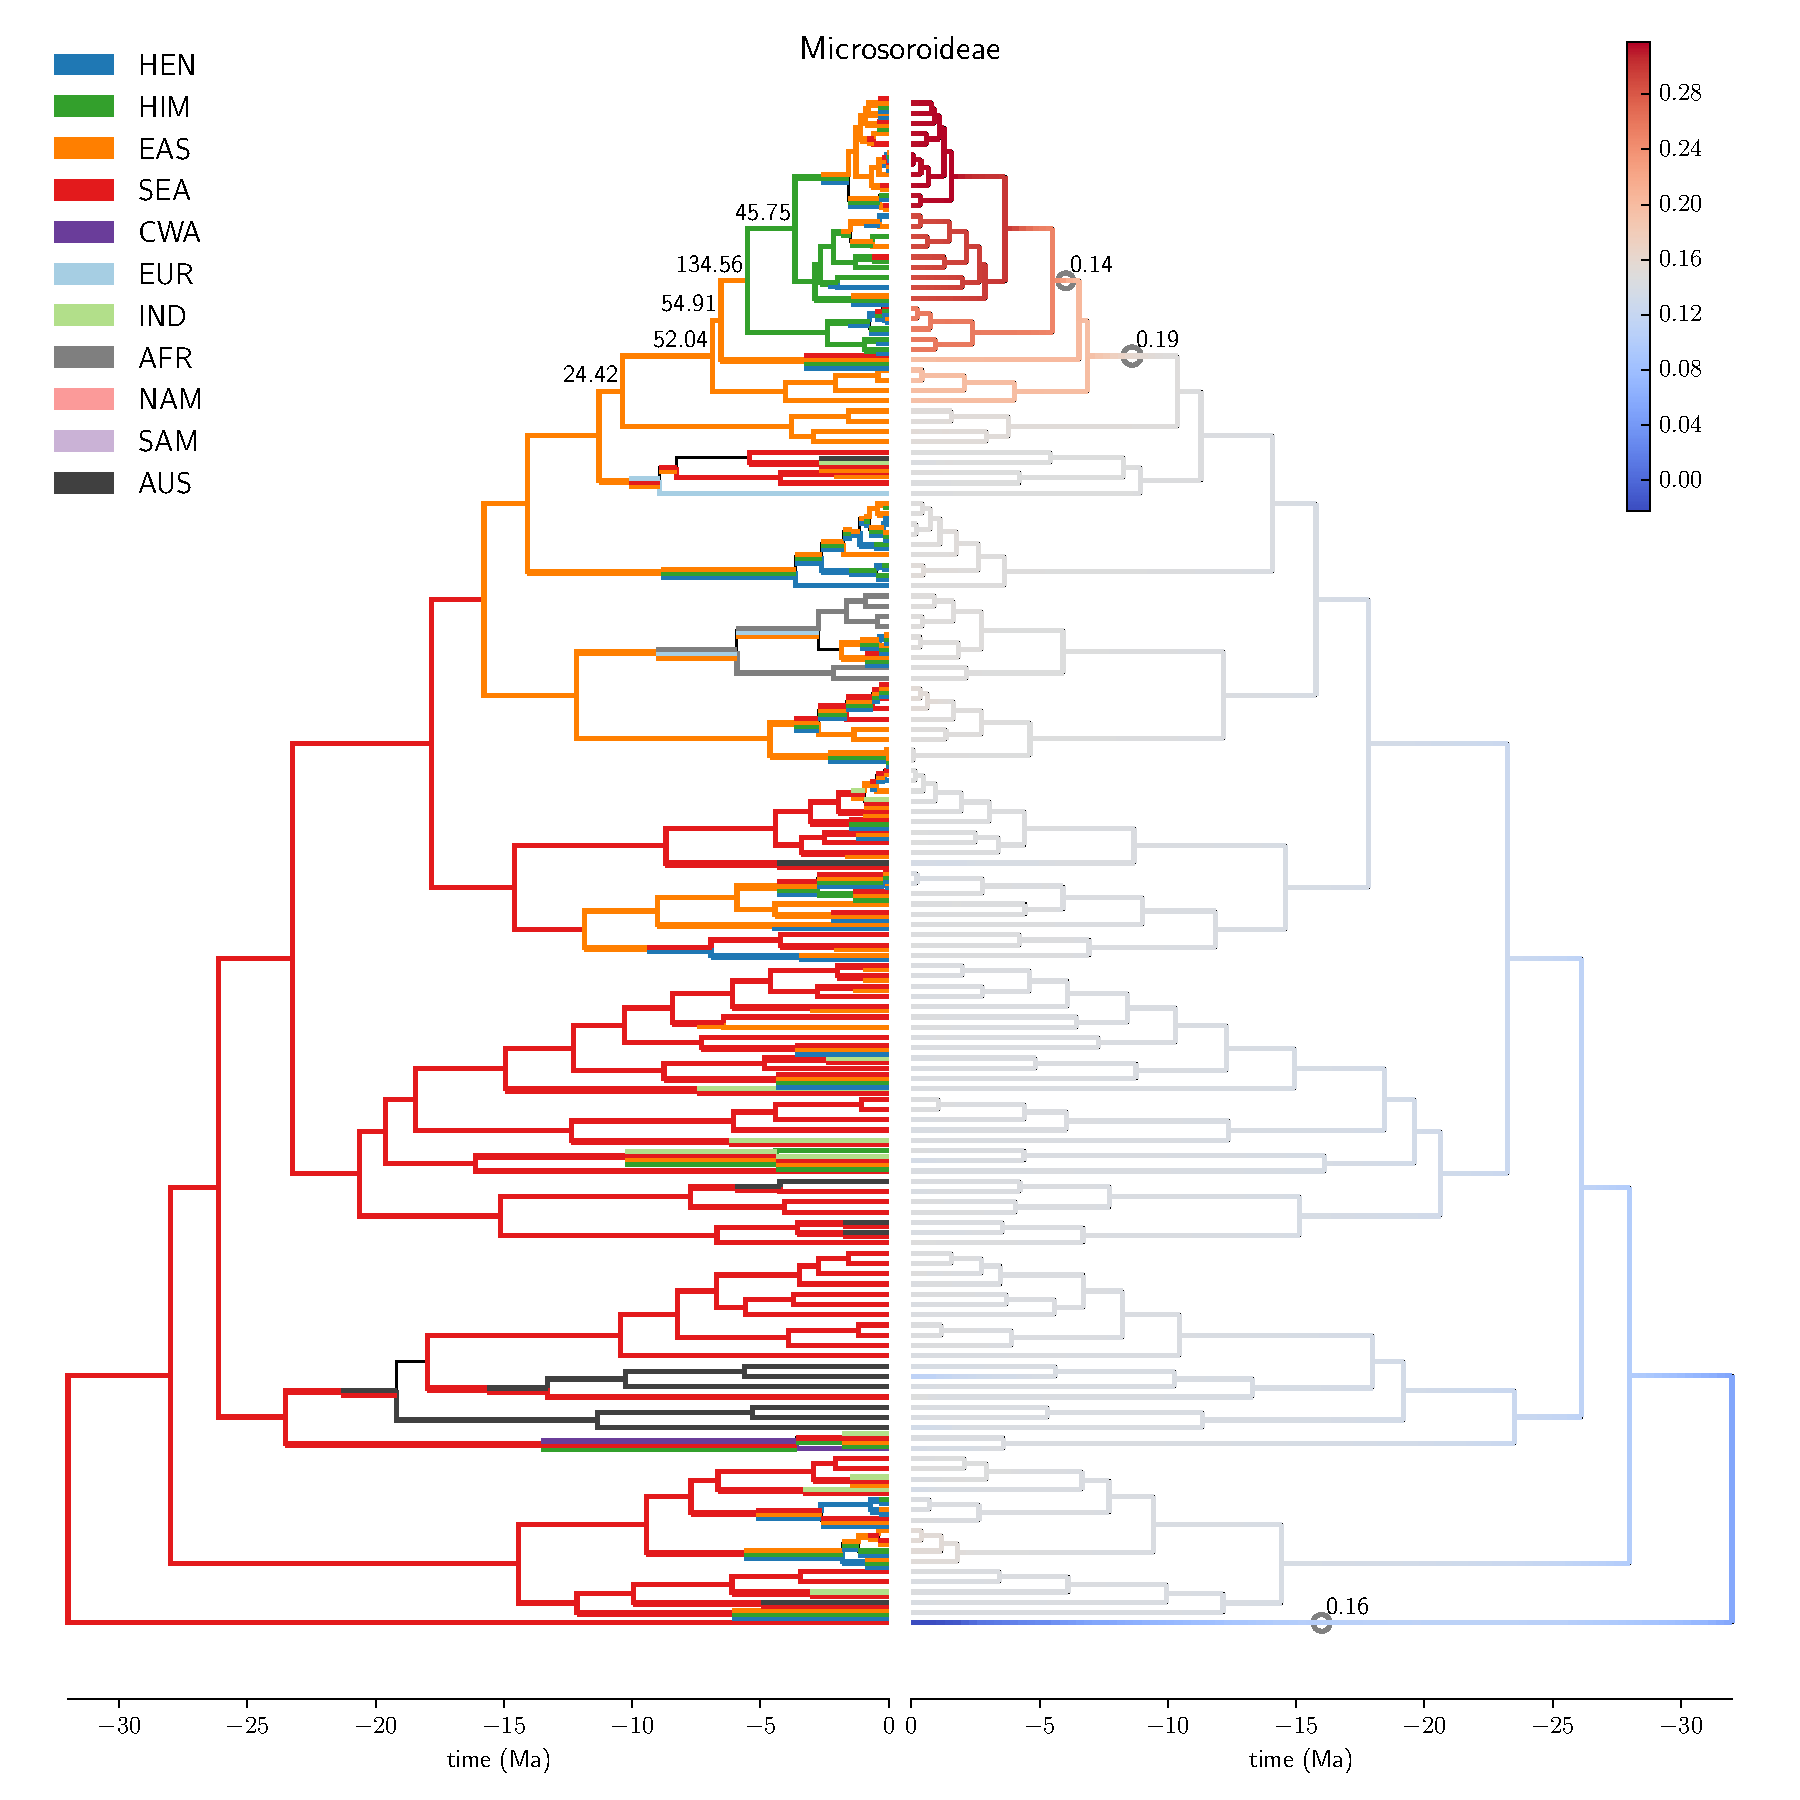
\includegraphics[width=.99\linewidth]{figures/Microsoroideae-supfig.pdf}
\label{fig:allium}
\caption{Microsoroideae}
\end{subfigure}
\end{figure}

\begin{figure}
  \ContinuedFloat
\begin{subfigure}{\textwidth}
\centering
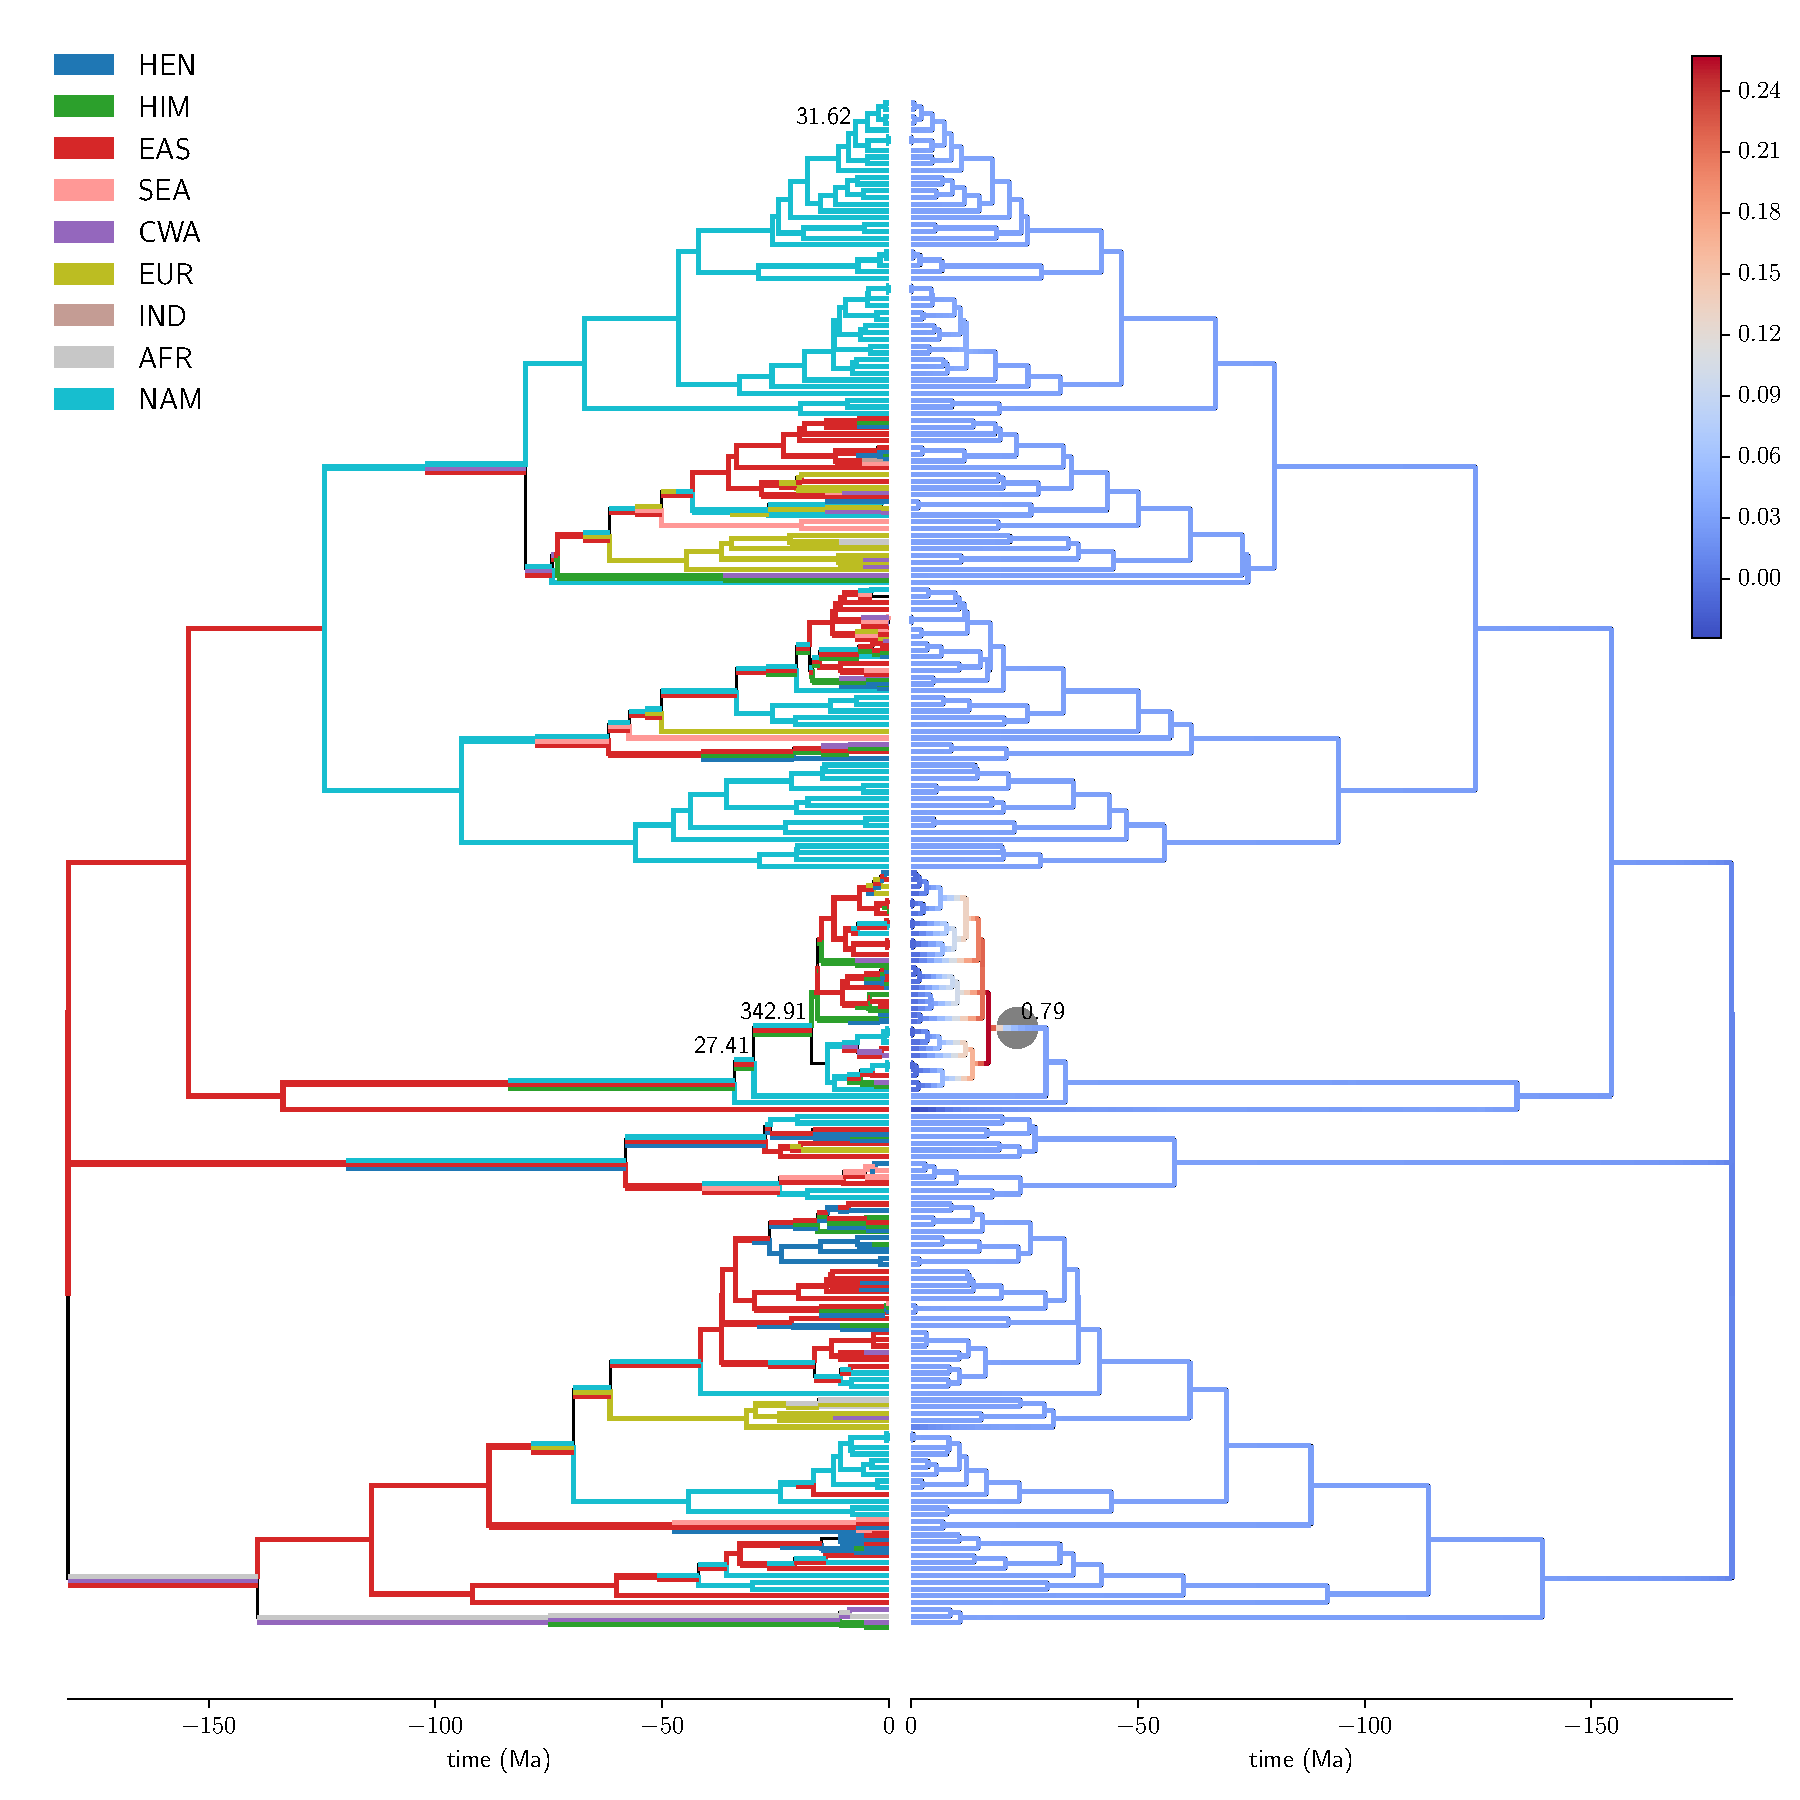
\includegraphics[width=.99\linewidth]{figures/Pinaceae-supfig.pdf}
\label{fig:allium}
\caption{Pinaceae}
\end{subfigure}
\end{figure}

\begin{figure}
  \ContinuedFloat
\begin{subfigure}{\textwidth}
\centering
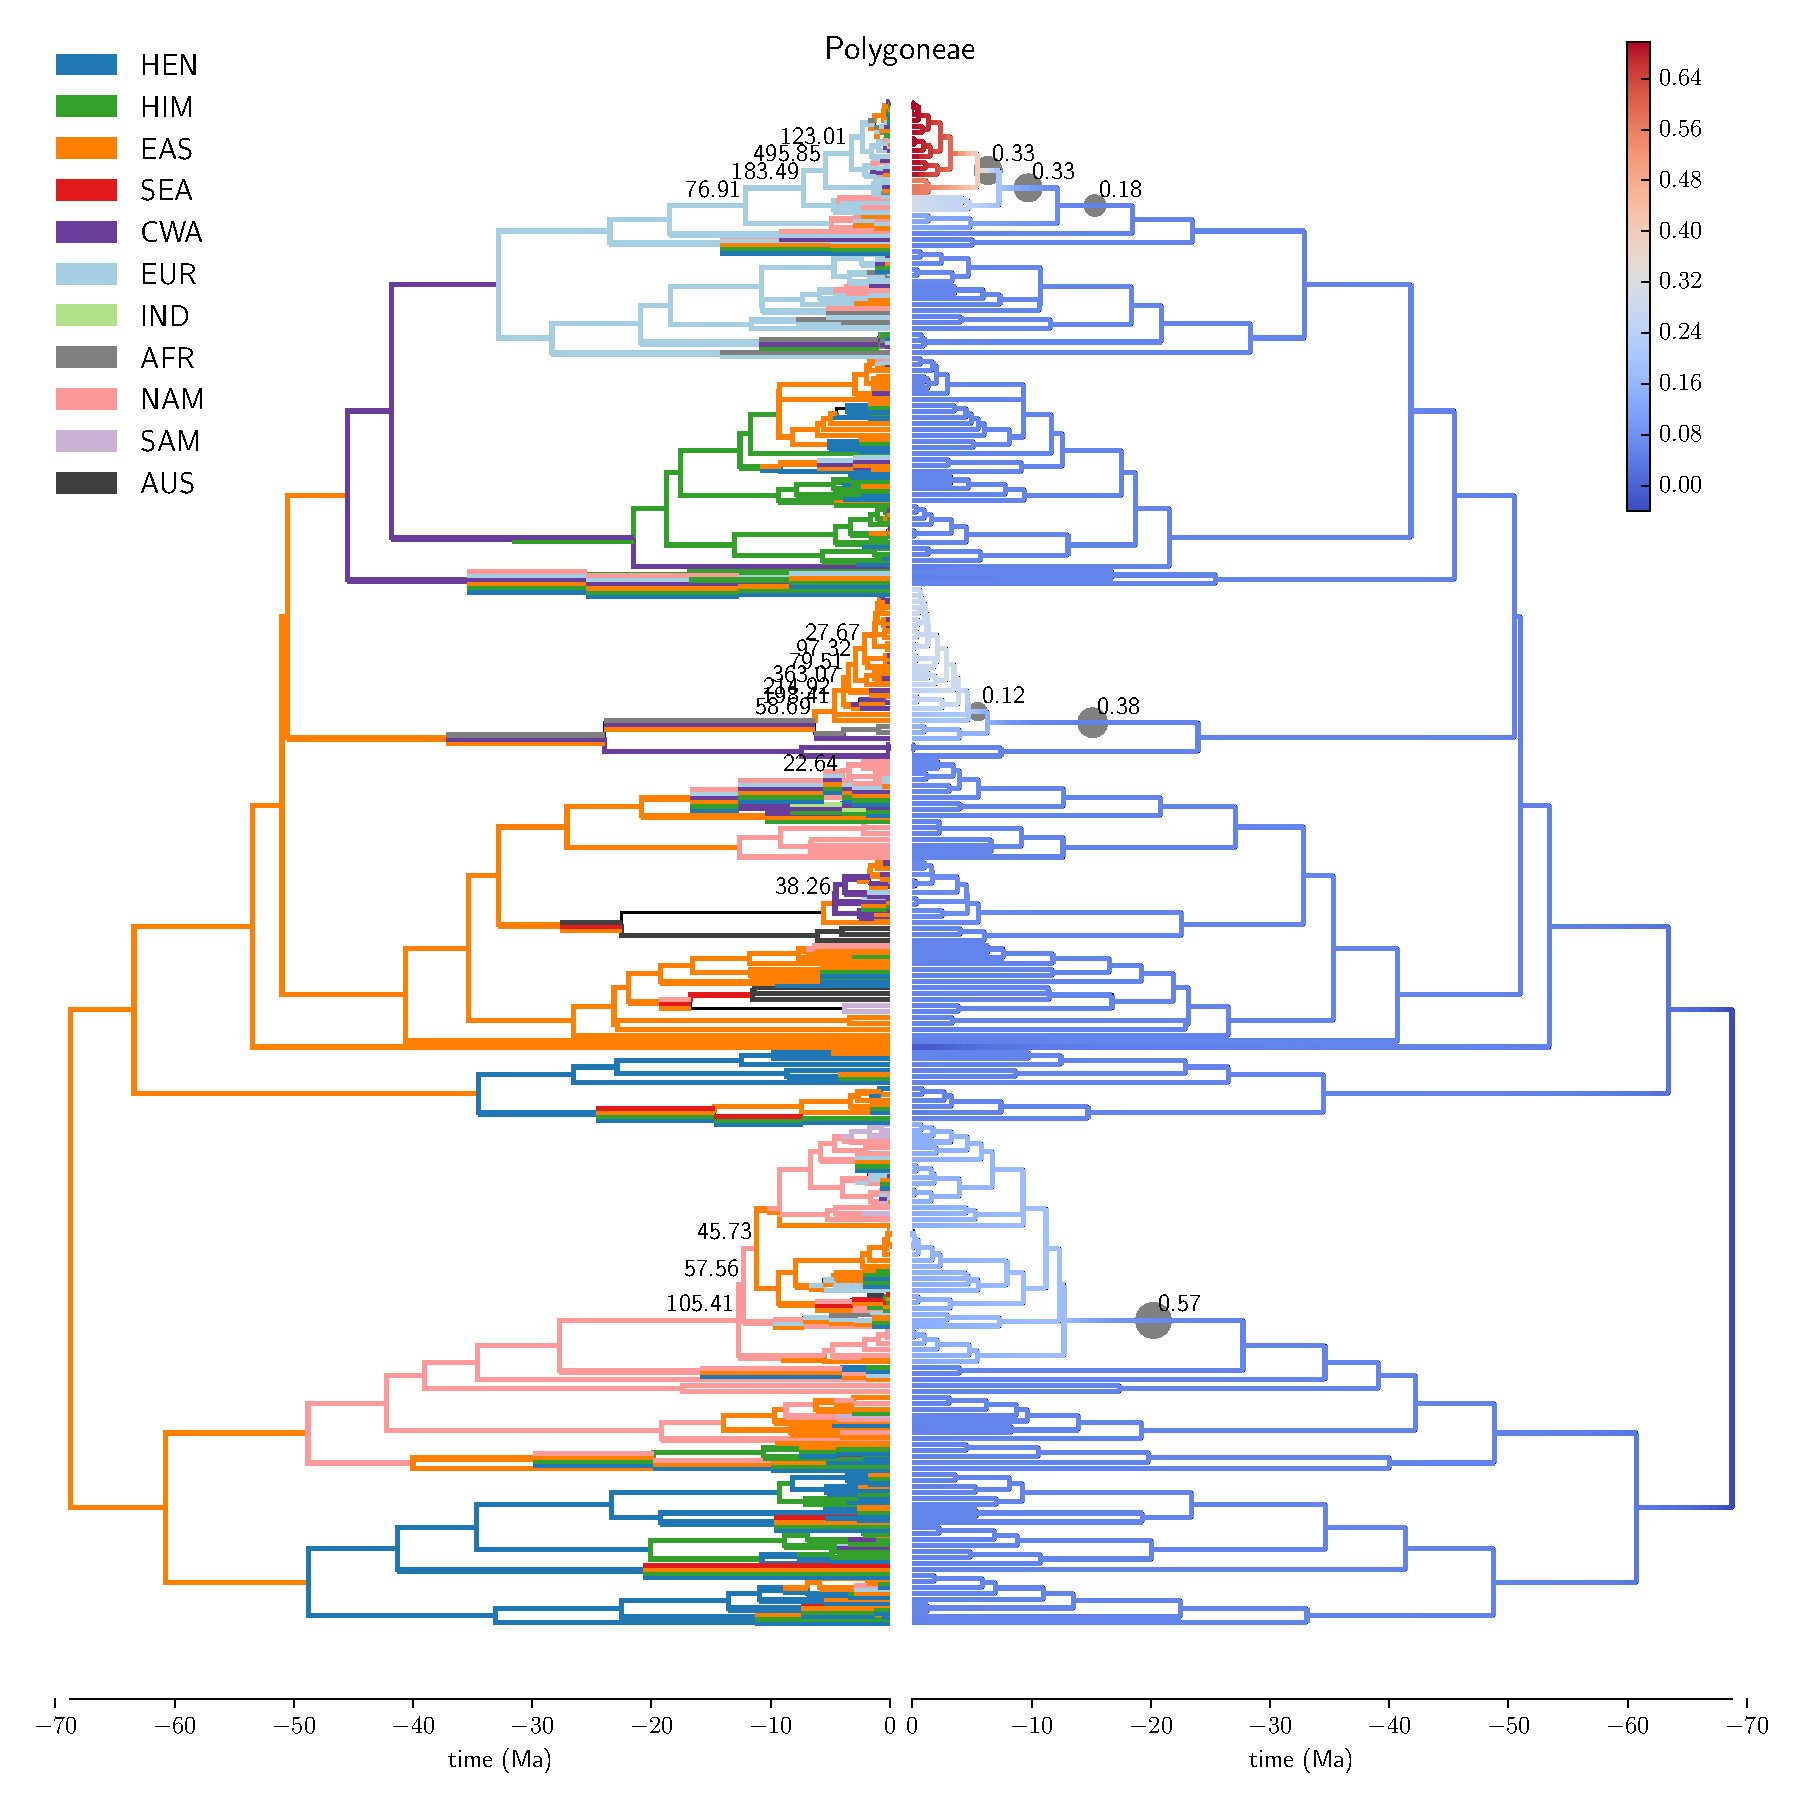
\includegraphics[width=.99\linewidth]{figures/Polygoneae-supfig.pdf}
\label{fig:allium}
\caption{Polygoneae}
\end{subfigure}
\end{figure}

\begin{figure}
  \ContinuedFloat
\begin{subfigure}{\textwidth}
\centering
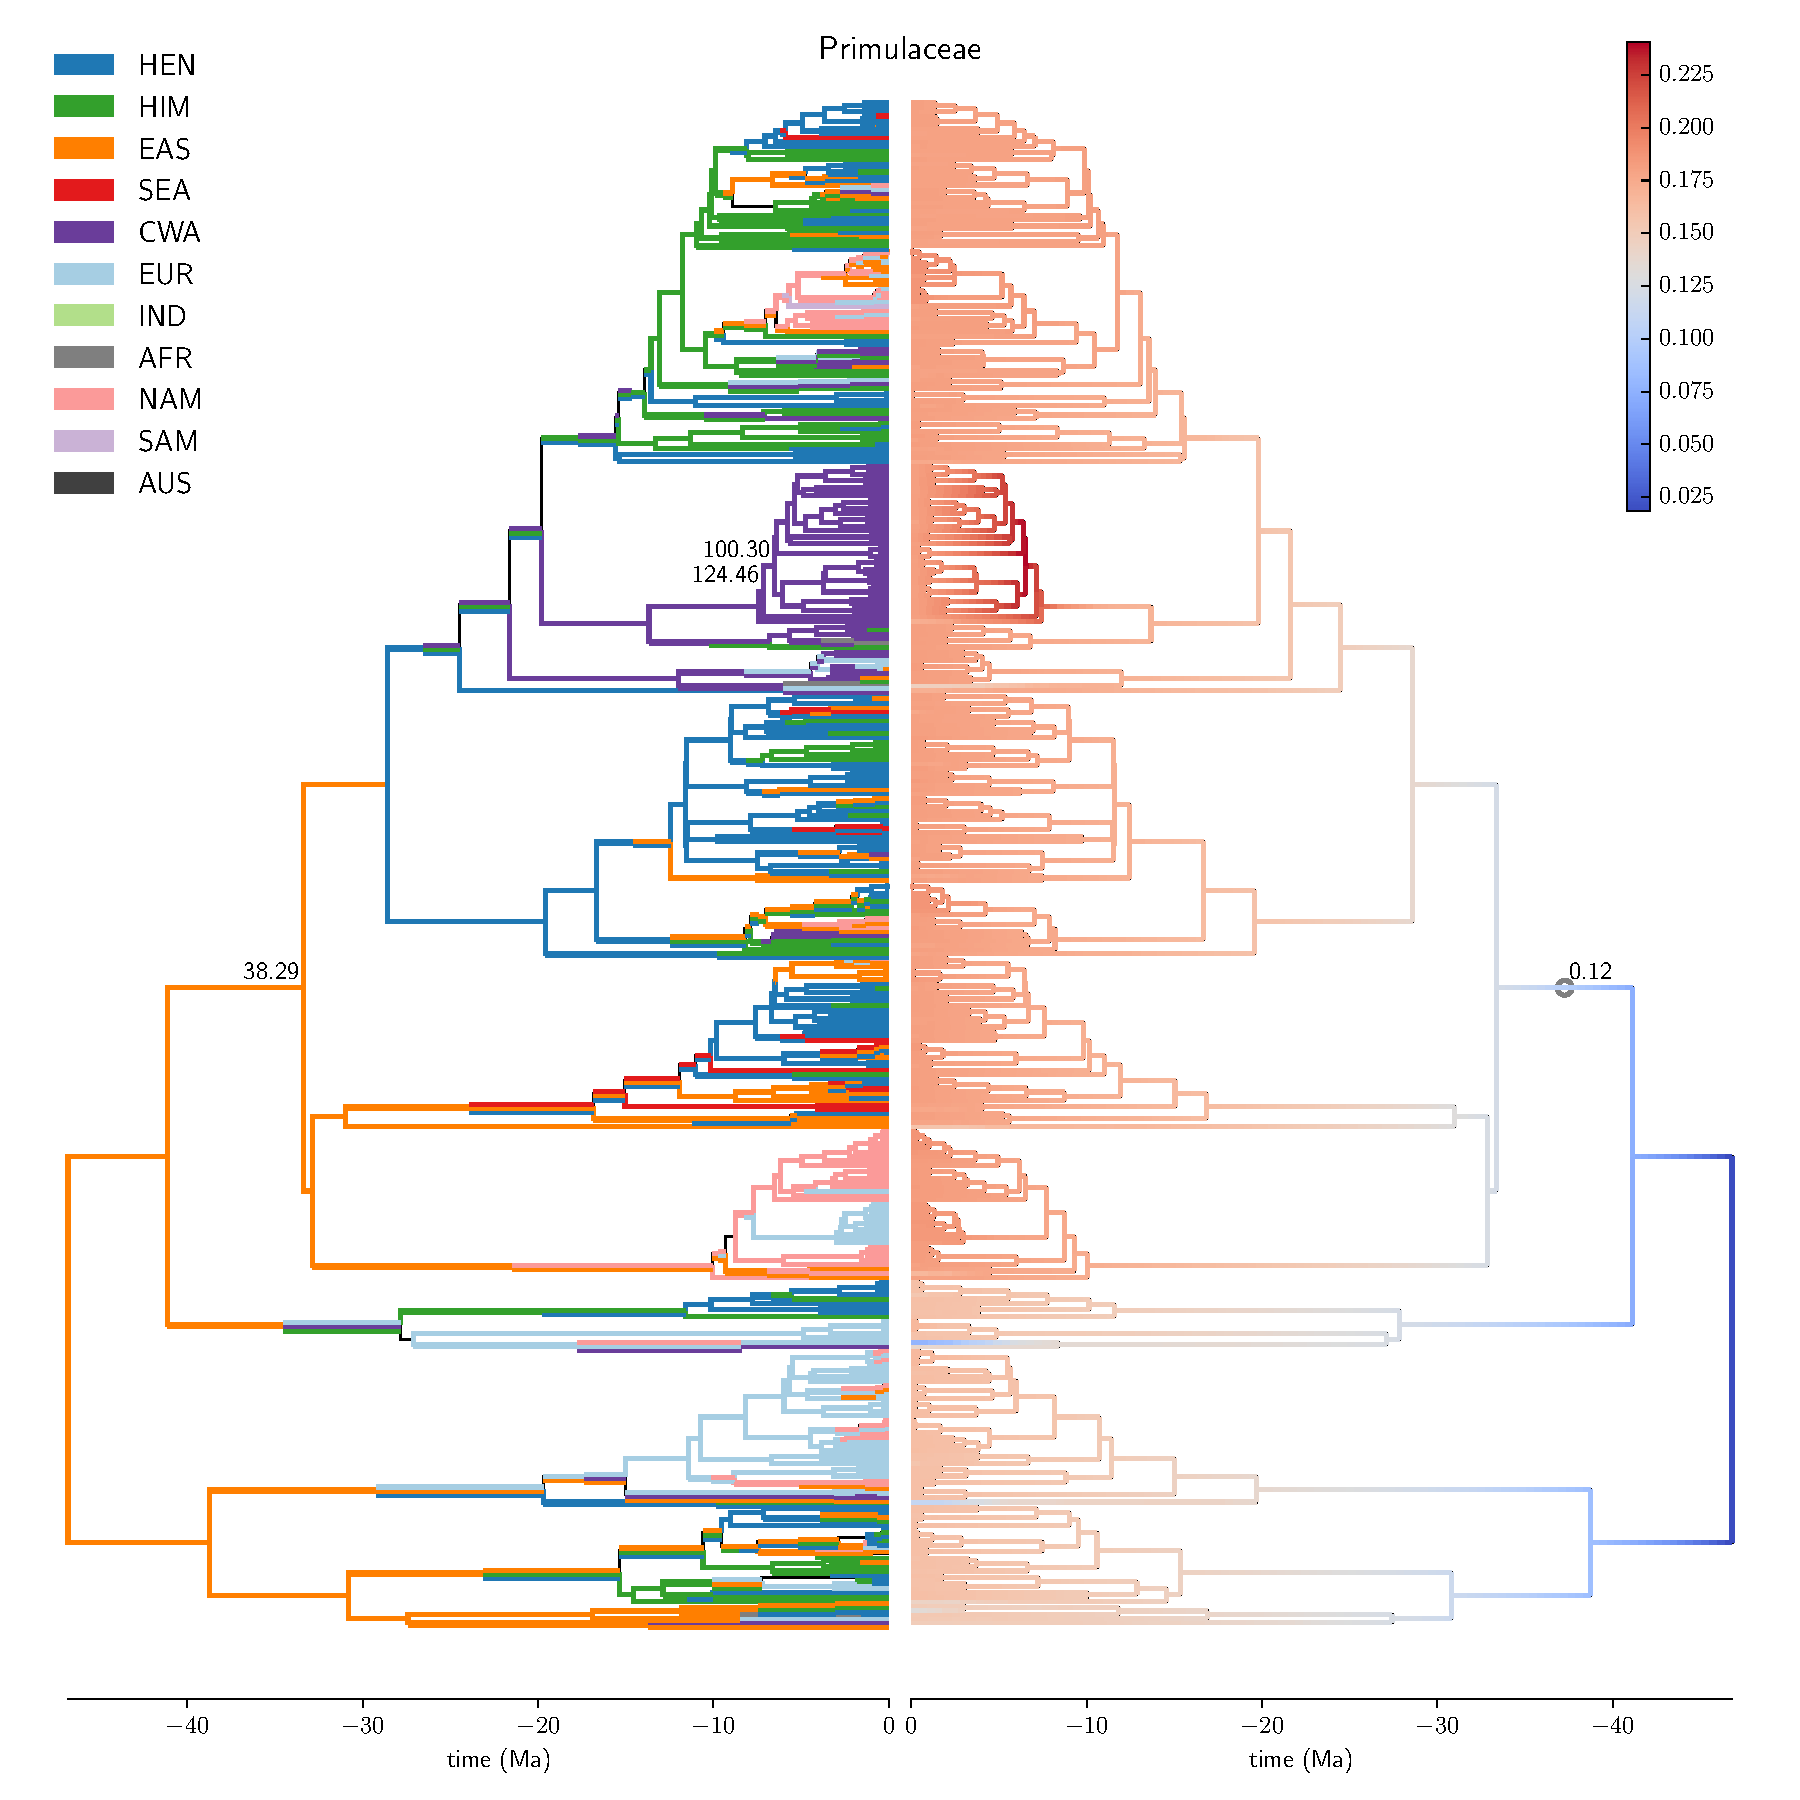
\includegraphics[width=.99\linewidth]{figures/Primulaceae-supfig.pdf}
\label{fig:allium}
\caption{Primulaceae}
\end{subfigure}
\end{figure}

\begin{figure}
  \ContinuedFloat
\begin{subfigure}{\textwidth}
\centering
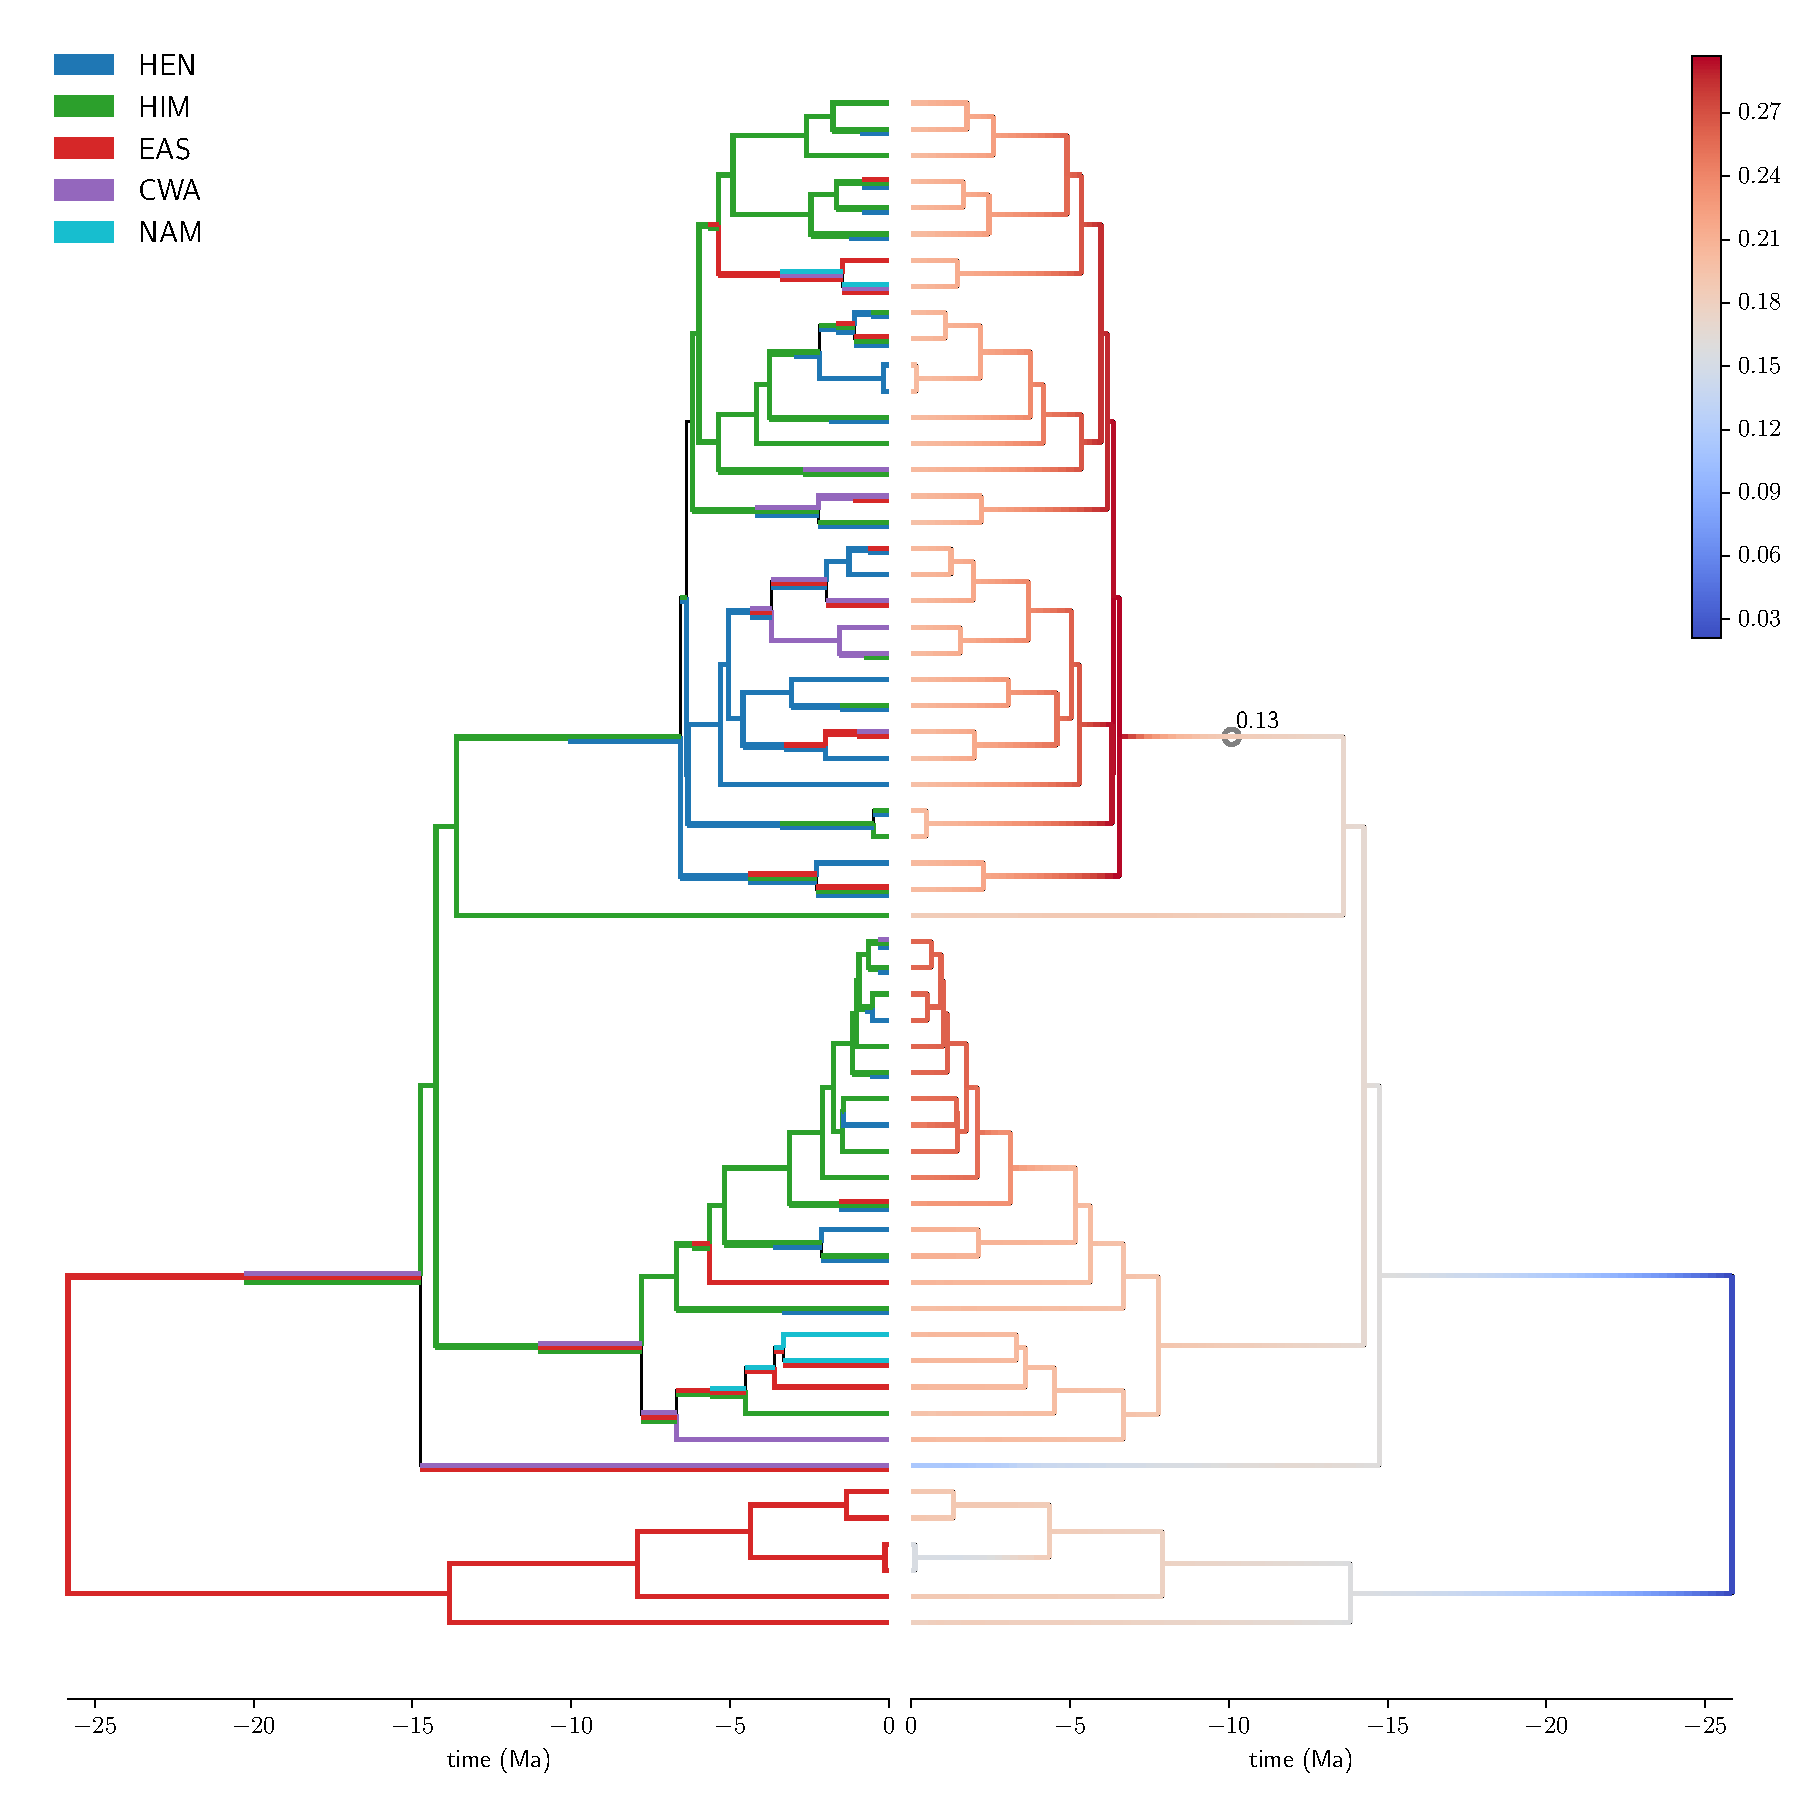
\includegraphics[width=.99\linewidth]{figures/Rhodiola-supfig.pdf}
\label{fig:allium}
\caption{\textit{Rhodiola}}
\end{subfigure}
\end{figure}

\begin{figure}
  \ContinuedFloat
\begin{subfigure}{\textwidth}
\centering
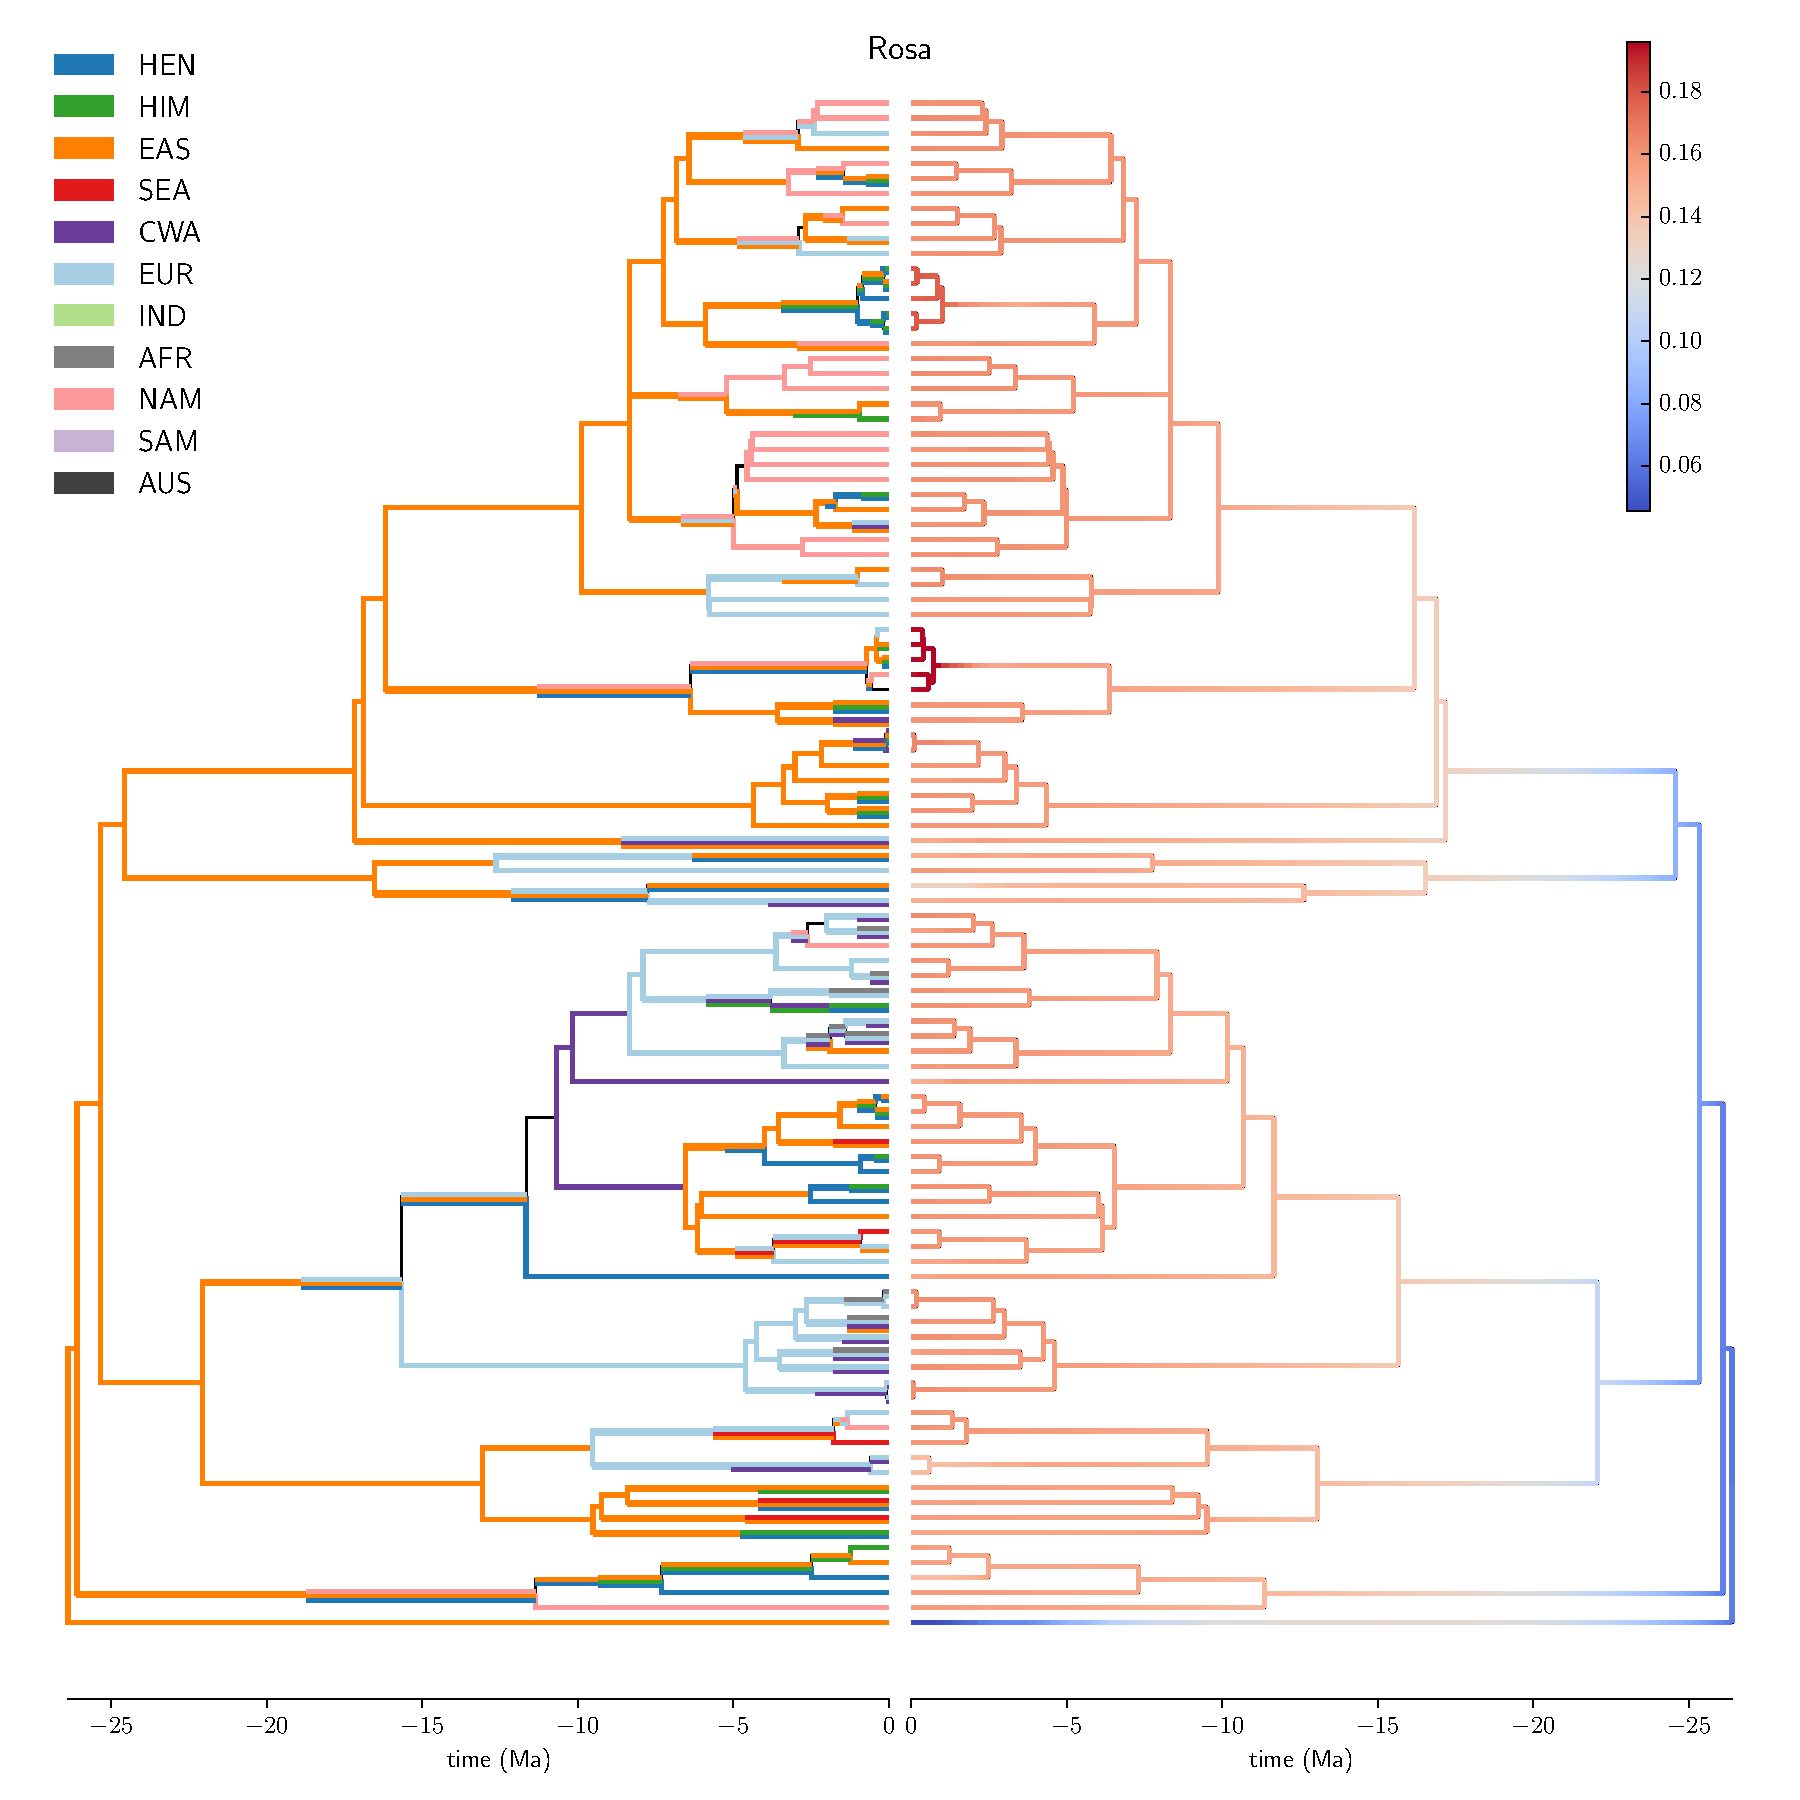
\includegraphics[width=.99\linewidth]{figures/Rosa-supfig.pdf}
\label{fig:allium}
\caption{\textit{Rosa}}
\end{subfigure}
\end{figure}

\begin{figure}
  \ContinuedFloat
\begin{subfigure}{\textwidth}
\centering
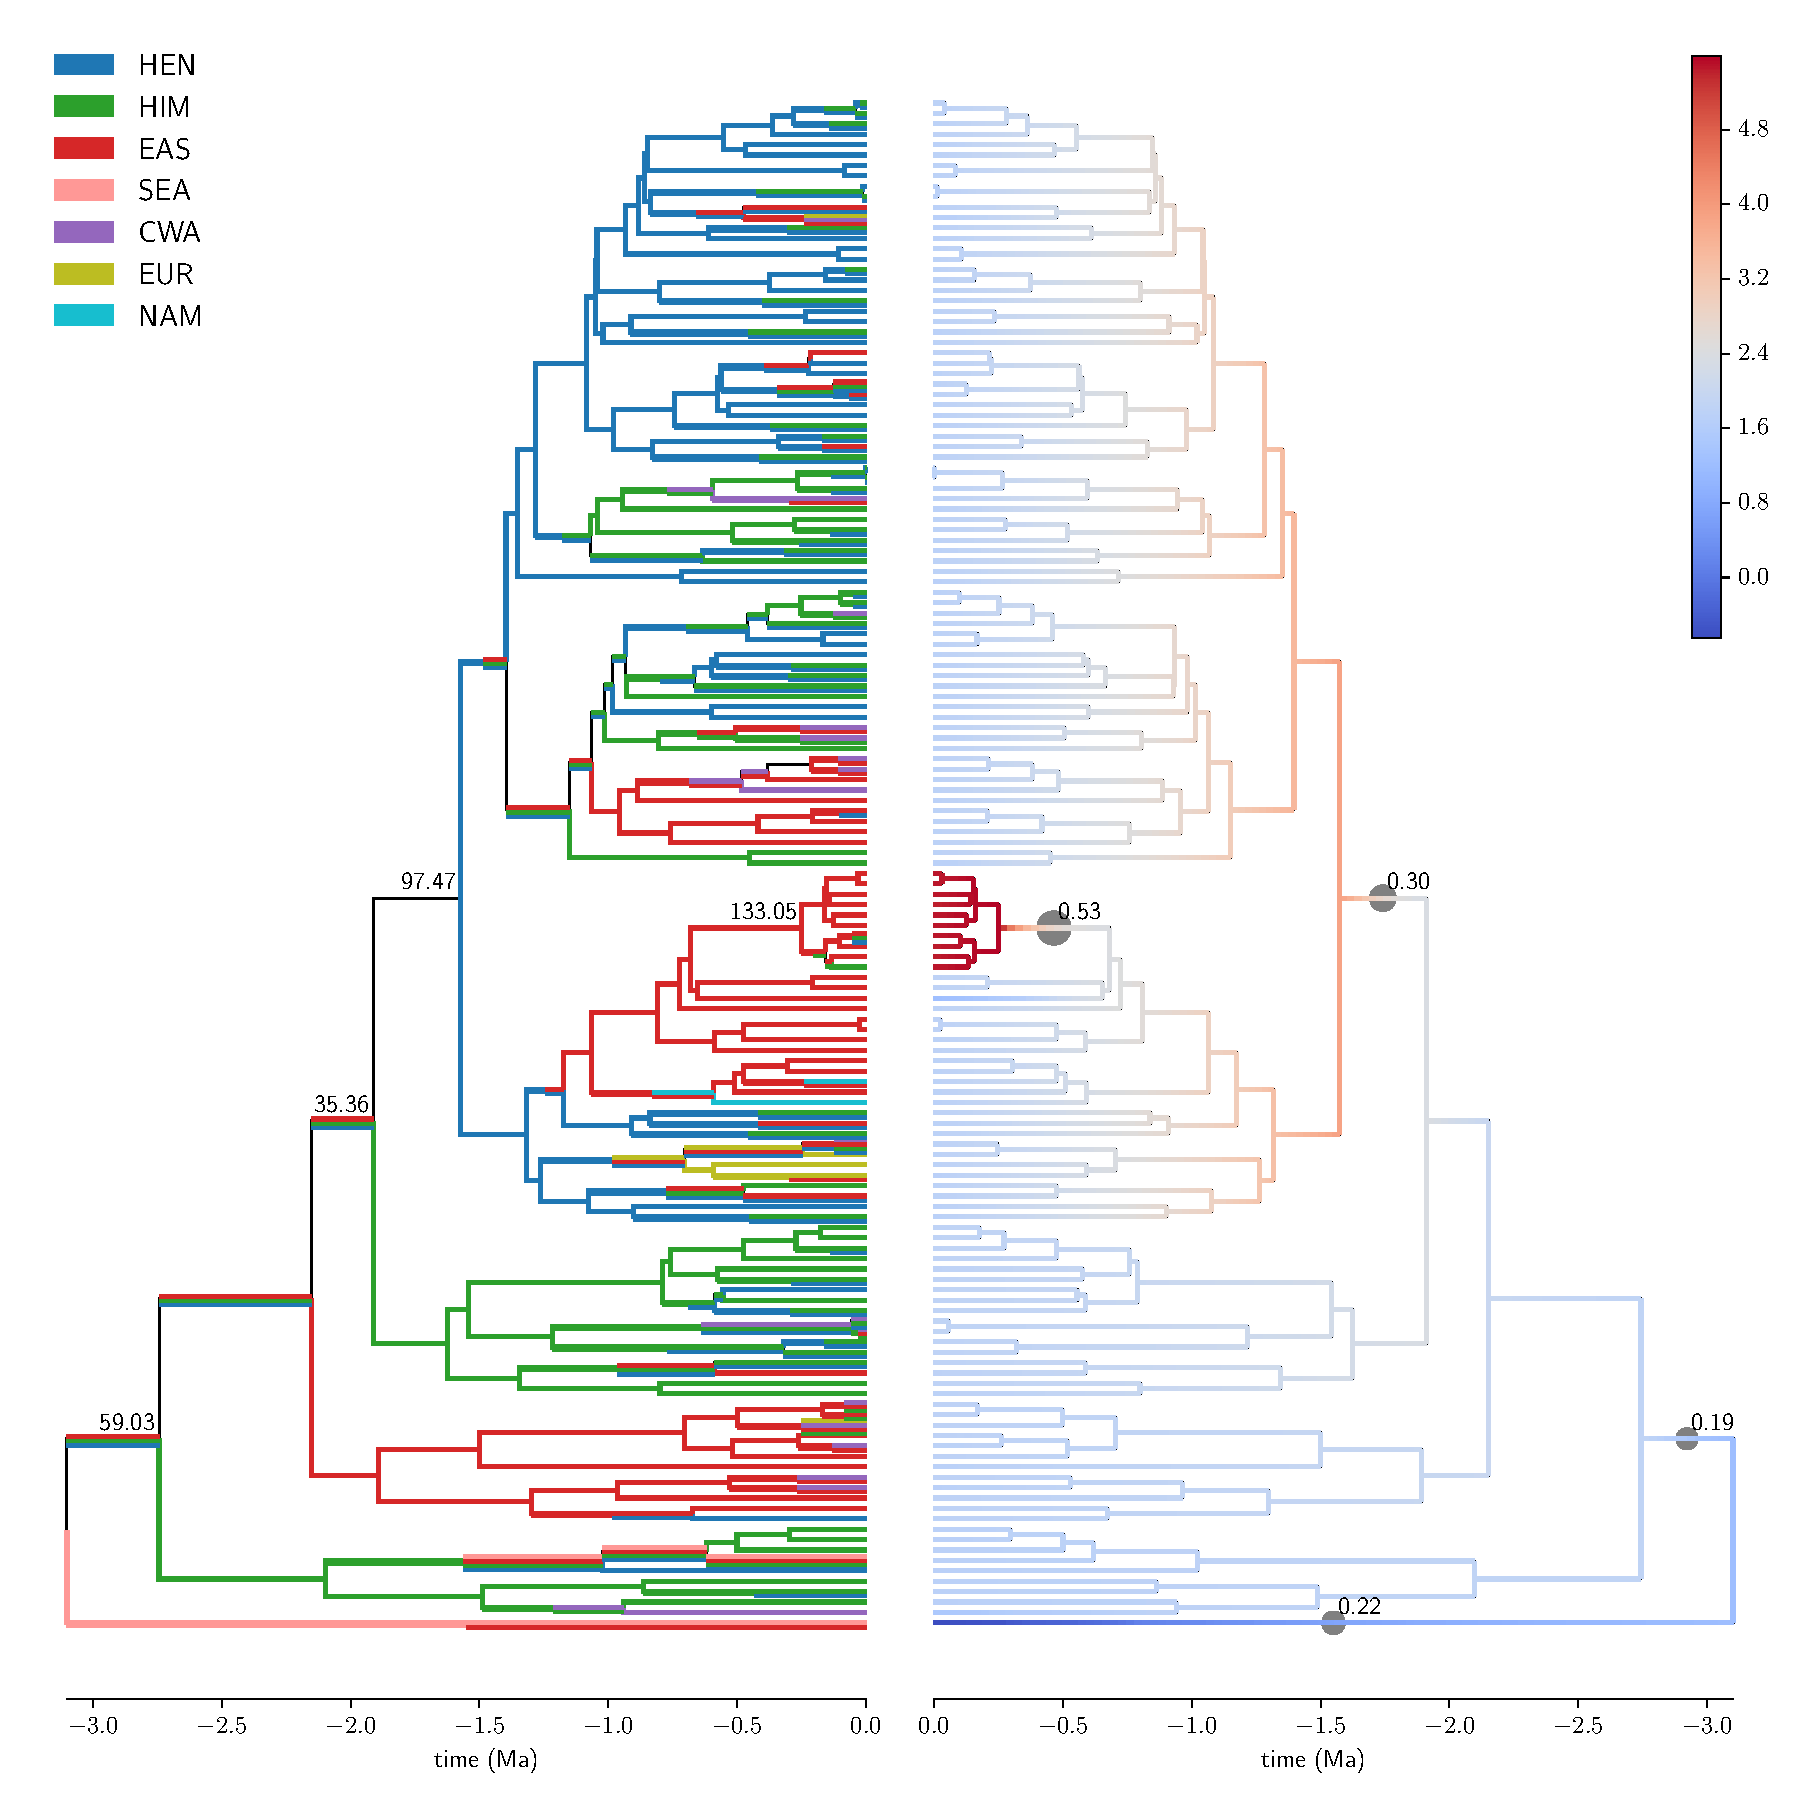
\includegraphics[width=.99\linewidth]{figures/Saussurea-supfig.pdf}
\label{fig:allium}
\caption{\textit{Saussurea}}
\end{subfigure}
\end{figure}

\begin{figure}
  \ContinuedFloat
\begin{subfigure}{\textwidth}
\centering
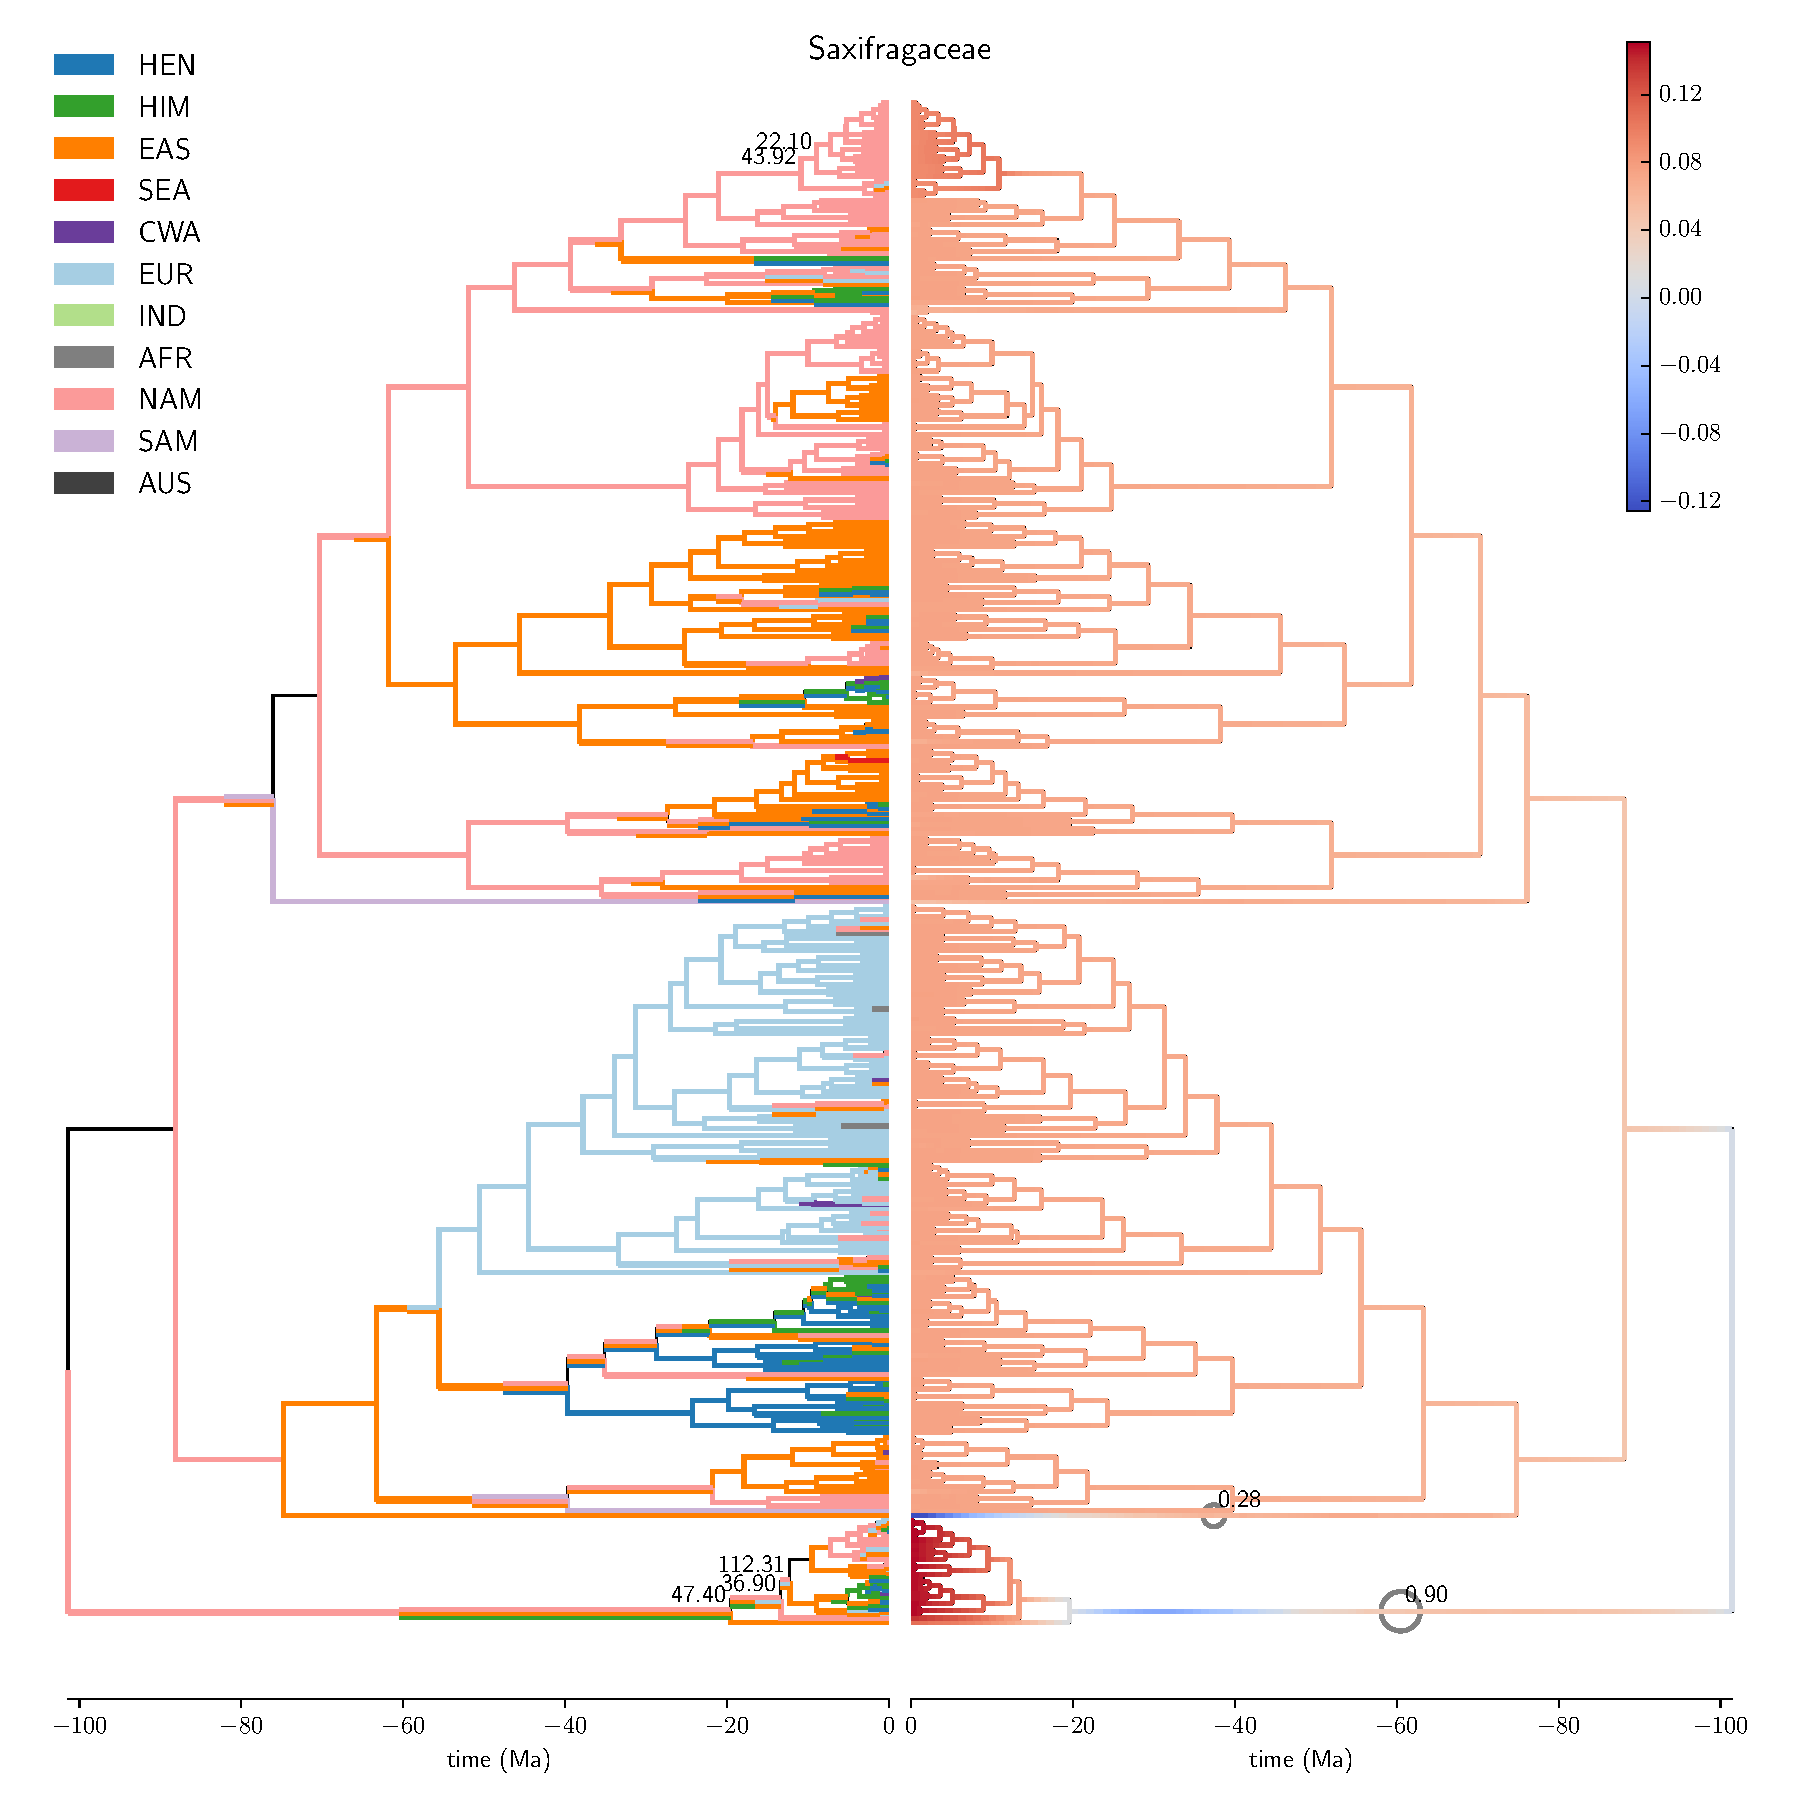
\includegraphics[width=.99\linewidth]{figures/Saxifragaceae-supfig.pdf}
\label{fig:allium}
\caption{Saxifragaceae-Grossulariaceae}
\end{subfigure}
\end{figure}

\begin{figure}
  \ContinuedFloat
\begin{subfigure}{\textwidth}
\centering
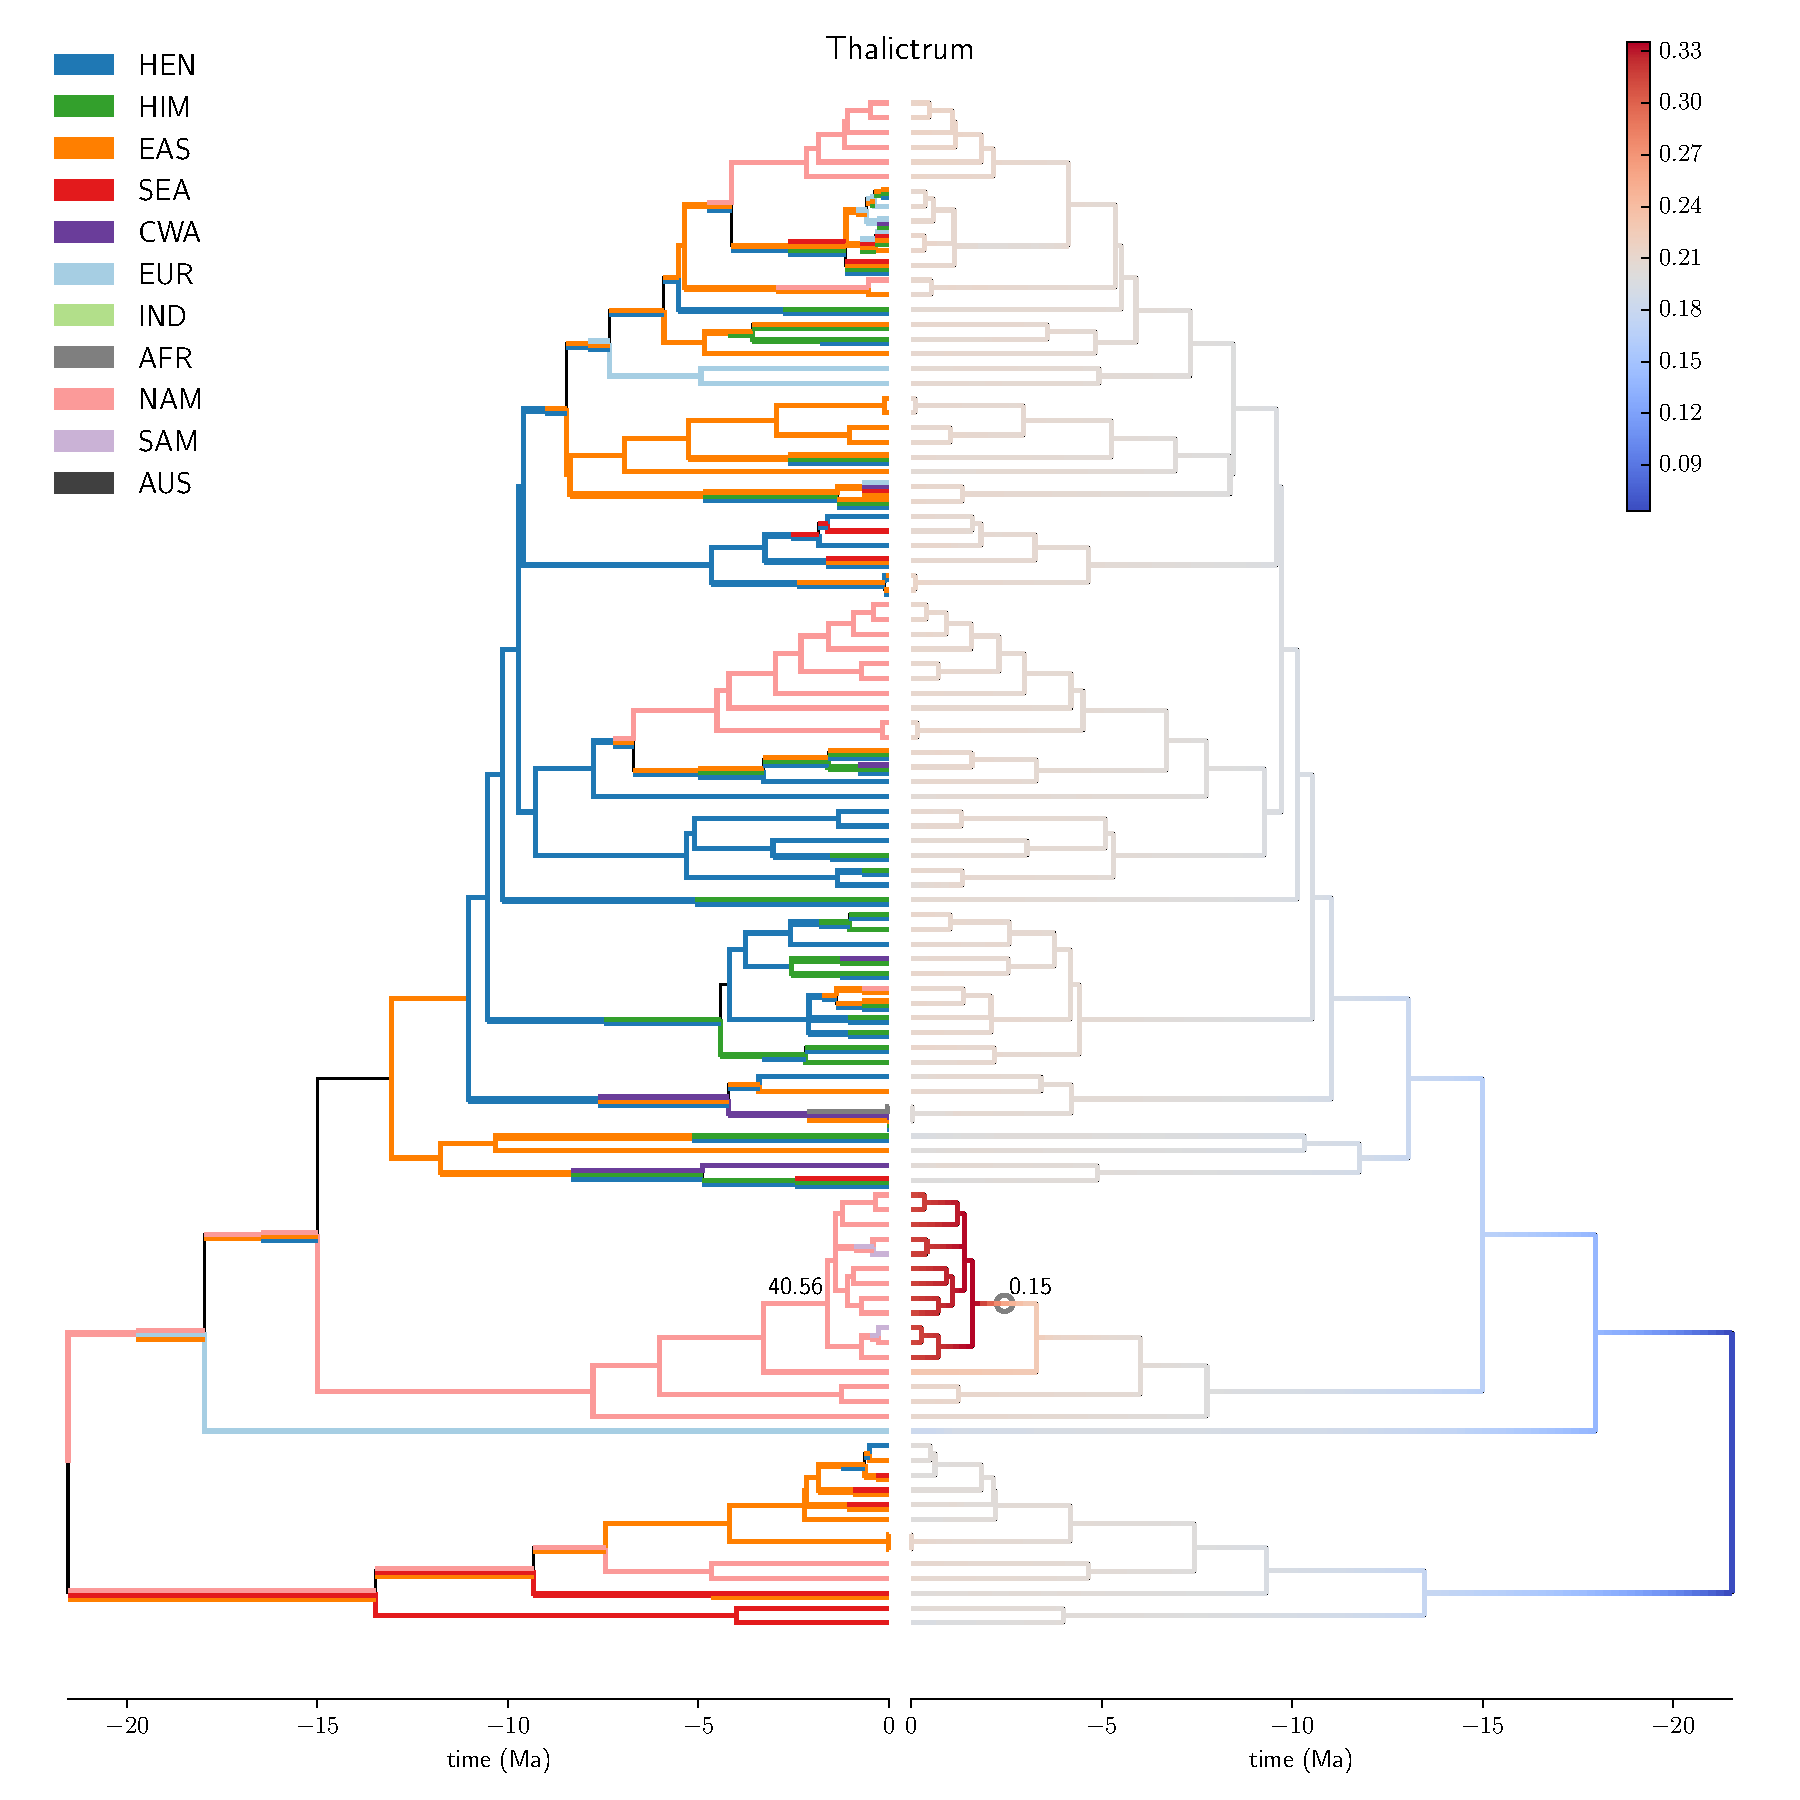
\includegraphics[width=.99\linewidth]{figures/Thalictrum-supfig.pdf}
\label{fig:allium}
\caption{\textit{Thalictrum}}
\end{subfigure}
\end{figure}

%%% Local Variables:
%%% mode: latex
%%% TeX-master: "SI"
%%% End:


%%% Local Variables:
%%% mode: latex
%%% TeX-master: "SI"
%%% End:
